%!TEX root=/home/ska124/Dropbox/Thesis/thes-full.tex
%% Copyright 1998 Pepe Kubon
%%
%% `thes-full.tex' --- the example thesis, FULL version, used
%%                     with  the `csthesis' package 
%% Use: latex thes-full to generate the DVI output, then 
%%      bibtex thes-full to generate the bibliography
%%      makeindex thes-full to get the index, and
%%      latex thes-full (2x) 
%%
%% You are allowed to distribute this file together with all files
%% mentioned in READ.ME.
%%
%% You are not allowed to modify its contents.
%%

\documentclass[11pt]{report}
%\documentclass[11pt,twoside]{report}%% for two-sided printing
\usepackage{pdfpages} 
\usepackage{anysize,fancyhdr,graphics}
\usepackage{csthesis}
\usepackage{makeidx}  %%% standard INDEX

\usepackage[titletoc]{appendix}%%Ensure word appendix appears in toc

%% Custom Packages 

\usepackage{subfig,graphicx}
\usepackage{array}
\usepackage{enumitem}
\usepackage{listings}


\makeindex  

%%% The following code demonstrates the ``other list'' facility. A new
%%% command \otherlist is defined for the List of Programs. Programs
%%% are defined as floating environments of type 3 (1 is used for figures,
%%% 2 for tables) and the information about them is stored in an
%%% auxiliary file with .lop extension. You can use this method to
%%% define several types of ``other lists,'' but in that case you'll
%%% need to add appropriate code to \lists in the csthesis.sty
%%% package.
%%% Note: It's better to move this code into your own mythesis.sty
%%% package. If you do that, you should get rid of the \makeatletter,
%%% \makeatother commands.
\makeatletter
\newcommand\otherlist{%
    \addcontentsline{toc}{chapter}{\otherlistname}
    \if@twocolumn
      \@restonecoltrue\onecolumn
    \else
      \@restonecolfalse
    \fi
    \chapter*{\otherlistname
      \@mkboth{\MakeUppercase\otherlistname}%
              {\MakeUppercase\otherlistname}}%
    \@starttoc{lop}%
    \if@restonecol\twocolumn\fi
    }
\newcommand*\l@program{\@dottedtocline{1}{1.5em}{2.3em}}
\newcommand\otherlistname{List of Programs}
\newcommand\programname{Program}
\newcounter{program}[chapter]
\renewcommand\theprogram{\thechapter.\@arabic\c@program}
\def\fps@program{tbp}
\def\ftype@program{3}
\def\ext@program{lop}
\def\fnum@program{\programname~\theprogram}

% Amoeba Cache
\def\AC{\textit{Amoeba-Cache}}
\def\AB{\textit{Amoeba-Block}}

%%%%%%%%%%%%%%%%%%%%%%%%%%%%%%%%%%%%%%%%%%%%%%%%%%%%%%%%%%%%%%%%%%%%%%
% mls: \code{...} command.
% Like \verb|...| but with braces, and not so fragile.
%
% Give me back the <, >, and _ characters in chosen modes
% unfortunately, this hack does not work when the <, >, or _ is embedded
% in another command.  In such circumstances use $<$, $>$, and \_
%
\makeatletter
\def\real@ltgtus{%
    \catcode`<=\active
    \catcode`>=\active
    \catcode`\_=\active
}
{\real@ltgtus
    \gdef<{\futurelet\@let@token\less@than}%
    \gdef>{\futurelet\@let@token\greater@than}%
    \gdef_{\underscore}%
}
% modify \textunderscore (standard LaTeX macro) to print as the _
% character in \tt font; as an appropriate rule in other fonts.
\renewcommand{\textunderscore}{\ifdim\fontdimen4\font=0pt\string_\else
    \leavevmode\kern.06em\vbox{\hrule width0.3em}\fi}
% \underscore is subscript in math mode, textunderscore otherwise
\DeclareRobustCommand{\underscore}{\ifmmode\sb\else\textunderscore\fi}
% similarly, create backslash, lessthan, and greaterthan macros that use
% the proper font:
\def\bs{\ifdim\fontdimen4\font=0pt\char92\relax\else
    \leavevmode$\backslash$\fi}
\newcommand{\less@than}{\ifdim\fontdimen4\font=0pt\string<\else
    \leavevmode\mathhexbox13C\fi}
\newcommand{\greater@than}{\ifdim\fontdimen4\font=0pt\string>\else
    \leavevmode\mathhexbox13E\fi}

% \code prints its argument in fixed-width font.
% There are no special characters in a code command, other than braces
% and backslash.
% It's similar to \verb, except that it's delimited normally (with
% braces).
\def\verythinspace{\kern .05em }
\DeclareRobustCommand{\code}{\begingroup
    \frenchspacing
    \real@ltgtus
    \@makeother\$\@makeother\&\@makeother\#%
    \@makeother\^\@makeother\%\@makeother\~%
    \@code}
\let\codefont\tt
\def\@code#1{\strut\verythinspace{\codefont
    #1}\verythinspace\strut\endgroup}
% For some reason I don't understand, escaped curly braces don't work
% right in \code commands.  Use the following instead:
\def\ttlb{{\tt\char123}}
\def\ttrb{{\tt\char125}}
\def\ttcaret{{\tt\char94}}
\def\tttilde{{\tt\char126}}
\makeatother
%%%%%%%%%%%%%%%%%%%%%%%%%%%%%%%%%%%%%%%%%%%%%%%%%%%%%%%%%%%%%%%%%%%%%%

%% Spots --- The round black magic blob

\def\spot#1{\begin{picture}(10,10)(-5,-4)%                                      
    \put(1,0){\circle*{10}}\put(-1,-3){\textcolor{white}{#1}}\end{picture}}

\def\bigspot#1{\begin{picture}(15,15)(-5,-5)%                                   
    \put(2,0){\circle*{15}}\put(-1,-3){\textbf{\textcolor{white}{#1}}}\end{picture}}



\newenvironment{program}
               {\@float{program}}
               {\end@float}
\newenvironment{program*}
               {\@dblfloat{program}}
               {\end@dblfloat}
\makeatother
%%% end of ``other list'' code

\begin{document}
\setlength{\pdfpagewidth}{8.5in}
\setlength{\pdfpageheight}{11in}
%%% set switches
%\contentspagefalse  
\figurespagetrue
\tablespagetrue
\dedicationpagetrue
\quotationpagetrue
% \otherlistpagetrue

%%% front matter 
%!TEX root=/home/ska124/Dropbox/Thesis/thes-full.tex
%% Copyright 1998 Pepe Kubon
%%
%% `titapp.tex' --- title and approval for thes-full.tex, thes-short-tex from
%%                  the `csthesis' bundle
%%
%% You are allowed to distribute this file together with all files
%% mentioned in READ.ME.
%%
%% You are not allowed to modify its contents.
%%

%%%%%%%%%%%%%%%%%%%%%%%%%%%%%%%%%%%%%%%%%%%%%
%
%   Title and approval pages
%
%%%%%%%%%%%%%%%%%%%%%%%%%%%%%%%%%%%%%%%%%%%%%

%%% title page

\title{Architectural support for a variable granularity cache memory system}
\author{Snehasish Kumar}
\qualification{B.Tech, Biju Patnaik University of Technology, 2010}
%\qualification{M.Xyf., Even Better University, 1994}
\submitdate{Fall 2012}
\copyrightyear{2012}

%%% approval page

\chair{Dr.~Hu Kaers} 
\signatory{Dr.~Arrvindh Shriraman, \\
        %% Assistant Professor, \\ Computing Science, \\
        %% Simon Fraser University\\ 
        Senior Supervisor}
\signatory{Dr.~Alexandra Federova, \\
        %% Professor, \\ Computing Science, \\
        %% Simon Fraser University\\ 
        Supervisor}
%%\signatory{Dr.~Hans Goof II,
%%       Professor, Computing Science\\
%%       Simon Fraser University\\ 
%        Co-Supervisor}
%% \signatory{Dr.~Silky Peach, Supervisor,\\
%%        Professor of Methodology,\\
%%        University of Nevada, Las Vegas
%%       }
%% \signatory{Dr.~Will Teachu,
%% %       Professor, Linguistics\\
%% %       Simon Fraser University\\ 
%%         SFU Examiner}
%% \signatory{Dr.~Will Testu, External Examiner,\\
%%         Professor of Unnatural Sciences,\\
%%         University of Surrey}

%%% generating title and approval pages 
\beforepreface

 %% title, approval

%% Partial Copyright License (PCL)
\newpage 			
\addcontentsline{toc}{chapter}{Partial Copyright License}
\mbox{}
\makeatletter
\AddToShipoutPictureBG*{
            \setlength{\@tempdimc}{.06\paperheight}
            \setlength{\unitlength}{1pt}
           \put(\strip@pt\@tempdimb,\strip@pt\@tempdimc){
	
\includegraphics{PCL_Declaration_2011.pdf}
	} 
} 
\makeatother
\newpage

%!TEX root=/home/ska124/Dropbox/Thesis/thes-full.tex
%% Copyright 1998 Pepe Kubon
%%
%% `abstract.tex' --- abstract for thes-full.tex, thes-short-tex from
%%                    the `csthesis' bundle
%%
%% You are allowed to distribute this file together with all files
%% mentioned in READ.ME.
%%
%% You are not allowed to modify its contents.
%%

%%%%%%%%%%%%%%%%%%%%%%%%%%%%%%%%%%%%%%%%%%%%%%%%%
%
%       Abstract 
%
%%%%%%%%%%%%%%%%%%%%%%%%%%%%%%%%%%%%%%%%%%%%%%%%

\prefacesection{Abstract}

Memory in modern computing systems are hierarchial in
nature. Maintaining a memory hierarchy enables the system to service
frequently requested data from a small low latency store located close
to the processor. The design paradigms of the memory hierachy have
been mostly unchanged since their inception in the late
1960's. However in the meantime there have been significant changes in
the tasks computers perform and the way they are programmed. Modern
computing systems perform more data centric tasks and are programmed
in higher level languages which introduce many layers of abstraction
between the programmer and the system. \\ 

Waste in the memory hierarchy refers to the under utilised space in
the memory system and consequently wasted energy and time. The data
access patterns of modern workloads are increasingly less uniform
which makes it hard to design a memory hierarchy with rigid design
principles that performs optimally for a wide range of workloads.  The
problem is exacerbated by the implications of the growing fraction of
dark silicon on a processor chip. \\

This dissertation proposes and evaluates the benefits of a novel
architecture for the on chip memory hierarchy which would allow it to
dynamically adapt to the requirements of the application. We propose a
design that can support a variable number of cache blocks, each of a
different granularity. It employs a novel organization that completely
eliminates the tag array, treating the storage array as uniform and
morphable between tags and data.  This enables the cache to harvest
space from unused words in blocks for additional tag storage, thereby
supporting a variable number of tags (and correspondingly, blocks).
The design adjusts individual cache line granularities according to
the spatial locality in the application.  It adapts to the appropriate
granularity both for different data objects in an application as well
as for different phases of access to the same data. \\

Compared to a fixed granularity cache, improves cache utilization to
90\% - 99\% for most applications, saves miss rate by up to 73\% at
the L1 level and up to 88\% at the LLC level, and reduces miss
bandwidth by up to 84\% at the L1 and 92\% at the LLC. Correspondingly
reduces on-chip memory hierarchy energy by as much as 36\% and
improves performance by as much as 50\%.
 %% abstract
%!TEX root=/home/ska124/Dropbox/Thesis/thes-full.tex
%% Copyright 1998 Pepe Kubon
%%
%% `dedquot.tex' --- dedication and quotation for thes-full.tex from
%%                   the `csthesis' bundle
%%
%% You are allowed to distribute this file together with all files
%% mentioned in READ.ME.
%%
%% You are not allowed to modify its contents.
%%

%%%%%%%%%%%%%%%%%%%%%%%%%%%%%%%%%%%%%%%%%%%%%
%
%   Dedication/Quotation pages
%
%%%%%%%%%%%%%%%%%%%%%%%%%%%%%%%%%%%%%%%%%%%%%

\dedication{Dedicated to Baba, Ma and Bukum}
%\thesquot{%
%``Don't worry, Gromit. Everything's under control!''\\[5pt]%
%--- The Wrong Trousers, \textsc{Aardman Animations}, 1993%
%}

%%% generate pages

\dedicquotation















 %% dedication and quotation, if any 
%!TEX root=/home/ska124/Dropbox/Thesis/thes-full.tex
%% Copyright 1998 Pepe Kubon
%%
%% `ack.tex' --- aknowledgments for thes-full.tex, thes-short-tex from
%%               the `csthesis' bundle
%%
%% You are allowed to distribute this file together with all files
%% mentioned in READ.ME.
%%
%% You are not allowed to modify its contents.
%%

%%%%%%%%%%%%%%%%%%%%%%%%%%%%%%%%%%%%%%%%%%%
%
%       Acknowledgment 
%
%%%%%%%%%%%%%%%%%%%%%%%%%%%%%%%%%%%%%%%%%%

\prefacesection{Acknowledgments}
Here go all the people you want to thank.








 %%  acknowledgments

%%%  generate contents, lists of figures, etc.
\lists

%% preface (foreword), if any
% %!TEX root=/home/ska124/Dropbox/Thesis/thes-full.tex
%% Copyright 1998 Pepe Kubon
%%
%% `preface.tex' --- preface for thes-full.tex from
%%                   the `csthesis' bundle
%%
%% You are allowed to distribute this file together with all files
%% mentioned in READ.ME.
%%
%% You are not allowed to modify its contents.
%%

%%%%%%%%%%%%%%%%%%%%%%%%%%%%%%%%%%%%%%%%%%%%%%%%%
%
%       Preface 
%
%%%%%%%%%%%%%%%%%%%%%%%%%%%%%%%%%%%%%%%%%%%%%%%%

\prefacesection{Preface}
Here go all the interesting reasons why you decided to write this thesis.

 

%%% prepare main section
\beforetext

%%% main matter - chapters
%!TEX root=/home/ska124/Dropbox/Thesis/thes-full.tex
%% Copyright 1998 Pepe Kubon
%%
%% `05-introduction.tex' --- 1st chapter for thes-full.tex, thes-short-tex from
%%                the `csthesis' bundle

%%%%%%%%%%%%%%%%%%%%%%%%%%%%%%%%%%%%%%%%%%%%%%%%%
%
%       Chapter 1 
%
%%%%%%%%%%%%%%%%%%%%%%%%%%%%%%%%%%%%%%%%%%%%%%%%

\chapter{Introduction}
\label{introduction}

Memory systems are an integral part of computer architecture whose overall design and organisation have remained unchanged since their inception. Early mainframe computers in the 1960's were known to use a hierarchical memory organisation. The memory technologies included semi-conductor, magnetic core, drum and disc. Initially, accessing memory was only slightly slower than register access however as the difference grew, the need to mitigate the delay incurred for a memory access became extremely important. The rate at which computations were performed kept increasing, however the rate at which data was fed to the processor from the memory system did not grow at the same rate. In order to alleviate the effects of slow memory, smaller faster memory was built close to the processor to cache frequently used data. Caching was used to fetch data and instructions into the fastest memory on CPU accesses to take advantage of faster lookups on reuse. The first documented use of a data cache was in the IBM System/360 Model 85 \cite{liptay68}. \\

In modern systems, with multiple levels in their memory hierarchy, a couple of levels closest to the processor are made from static random access memory (SRAM) which increase in size as the distance from the processor increases. These are placed on the same die as the processor chip. To service a memory request not present in the previous levels, a request is sent off chip to fetch the data from main memory, constructed from dynamic random access memory (DRAM). The main memory is usually several magnitudes of order larger than the largest cache present on the chip. This can be afforded by the lower cost of DRAM compared to SRAM. However, DRAM lookups are slower and require more power to retain data. The speed, cost and size for each level in the memory hierarchy can be visualized as shown in Fig \ref{fig:memory_hierarchy}.

\begin{figure}[ht]
  %% Overview Cache Hierarchy
  \begin{center}
    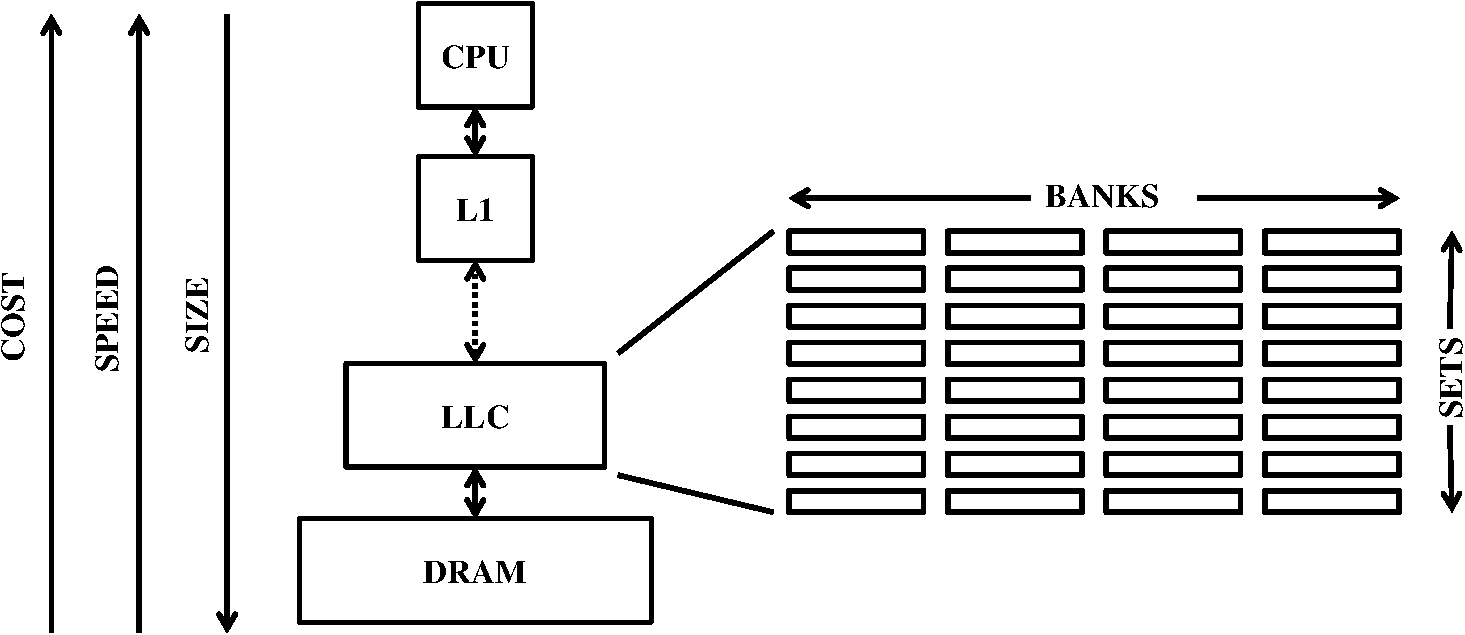
\includegraphics[width=\textwidth]{files/Figures/05-MemoryHierarchy.pdf}
    \caption[Canonical Memory Hierarchy]{\textbf{Canonical Memory Hierarchy} -- Moving down through the hierarchy, away from the processor, the levels are larger but slower. At each level the storage may be monolithic or sub divided in to "banks" for lower indexing overhead.}
    \label{fig:memory_hierarchy}
  \end{center}
\end{figure}

\section{Cache Memory Systems}
\label{sec:cache_memory_systems}
Most processors access data at the granularity of 4 to 8 bytes at a time. In order to exploit locality present in programs, caches are designed to retain small amounts of data close to the processor for fast access. The management of data in the cache is determined by a suitably selected replacement scheme. Caches are given designations to indicate their level in the memory hierarchy. The closest cached data stores to the processor are given lower numerical designations starting from \textit{L1} and increases as their distance from the processor increases. The last level of cache is often abbreviated as the \textit{LLC}. Each level in the cache hierarchy is linked in a daisy chain fashion, as shown in Fig \ref{fig:memory_hierarchy}, where there is an option for the data that is being cached to be replicated or not. The design choices can be enumerated as:

\begin{enumerate}
  \item Inclusive Caches : Lower level caches (further from the processor) replicate the cache lines present (although the data may be stale) present in the higher level caches. Inclusive caches can be found in Intel Sandy Bridge processors.
  \item Exclusive Caches : Caches lower in the hierarchy are guaranteed to not contain the cache lines present in the higher levels of the hierarchy. Present in the AMD architectures such as the Athlon processors.
  \item Non-Inclusive Caches : Also known as \textit{Non-Exclusive} or \textit{Accidentally Inclusive}, were used for a while in Intel architectures prior to the Intel P6. A lower level cache may or may not include a block cached at a higher level in the cache hierarchy.
\end{enumerate}

Caches are designed to take advantage of reuse of data by speeding up subsequent access to the same datum. They also speed up accesses to nearby data which may be fetched into the cache depending on its operating policy. The different types of locality which caches try to exploit can be enumerated as :

\begin{enumerate}
  \item Temporal Locality : Some applications tend to reuse the same data items over and over again during the course of their execution. This principle is the cornerstone for caching. Cache management policies usually implemented take into account the recency of data reuse to take a decision on what data is to be retained in the cache. Modern cache hierarchies implement a form of the \textit{Least Recently Used} algorithm to manage the contents of the cache.
  \item Spatial Locality : Due to conventional imperative programming paradigms, data is usually managed by grouping datum together in data structures, the fields of which are accessed in close proximity in the source code. Thus in order to exploit this pattern when a datum is requested, it is normal behaviour for the cache to bring in a contiguous region, 32 -- 128 bytes in size, which contains the datum. The contiguous region of data brought into the cache is referred to as a \textit{cache block} or \textit{cache line}. The Intel Pentium 3 processors used a 32 byte line size which was increased to 64 bytes from Pentium 4. The IBM Power7 architectures use a 128 byte cache line where as the Intel Itanium2 uses a 64 bytes cache line size at the L1 and 128 byte cache line size at the L2 and L3.
\end{enumerate}

According to the place where a new cache line can be inserted into the cache, the cache can have varying associativity. If the policy requires that a certain block from memory can map only to a specific entry in the cache, it is known as a \textit{direct mapped} cache [Fig \ref{fig:cache_associativity}(a)]. On the other end of the spectrum, if a certain block from memory can map to any entry in the cache it is known as a \textit{fully associative} cache [Fig \ref{fig:cache_associativity}(c)].  It is easy to see that fully associative caches are the most flexible, however they incur significant costs in terms of latency and area overhead for standard cache operations. A cache lookup for a specific block is analogous to checking each item in a collection for a possible match. Conventional caches are organised as a 2-dimensional data structure where the rows are called \textit{sets}. Within each set there are a fixed number of cache blocks. The number of blocks in each set is the degree of associativity of the cache. Each possible entry in a set is called a \textit{way}. Thus a direct mapped cache has associativity of 1 where as a fully associative cache is one whose associativity is equal to the total number of cache blocks that the given cache can possibly hold.  


\begin{figure}[h]
  %% Get images from http://en.wikipedia.org/wiki/CPU_cache#Associativity
  \subfloat[Direct Mapped]{
    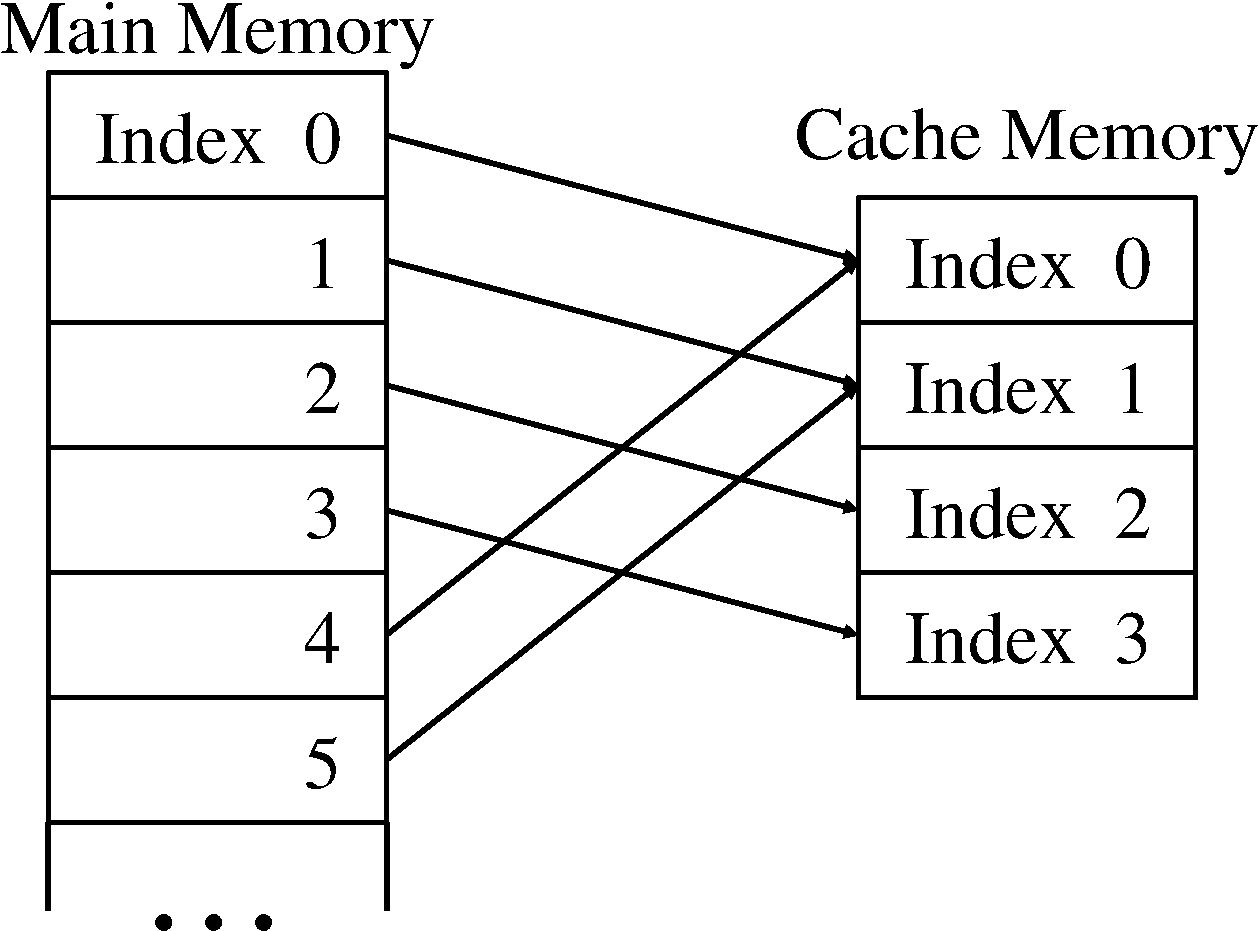
\includegraphics[width=0.32\textwidth]{files/Figures/05-DirectMapped.pdf}
  }
  \subfloat[2-way Set Associative ]{
     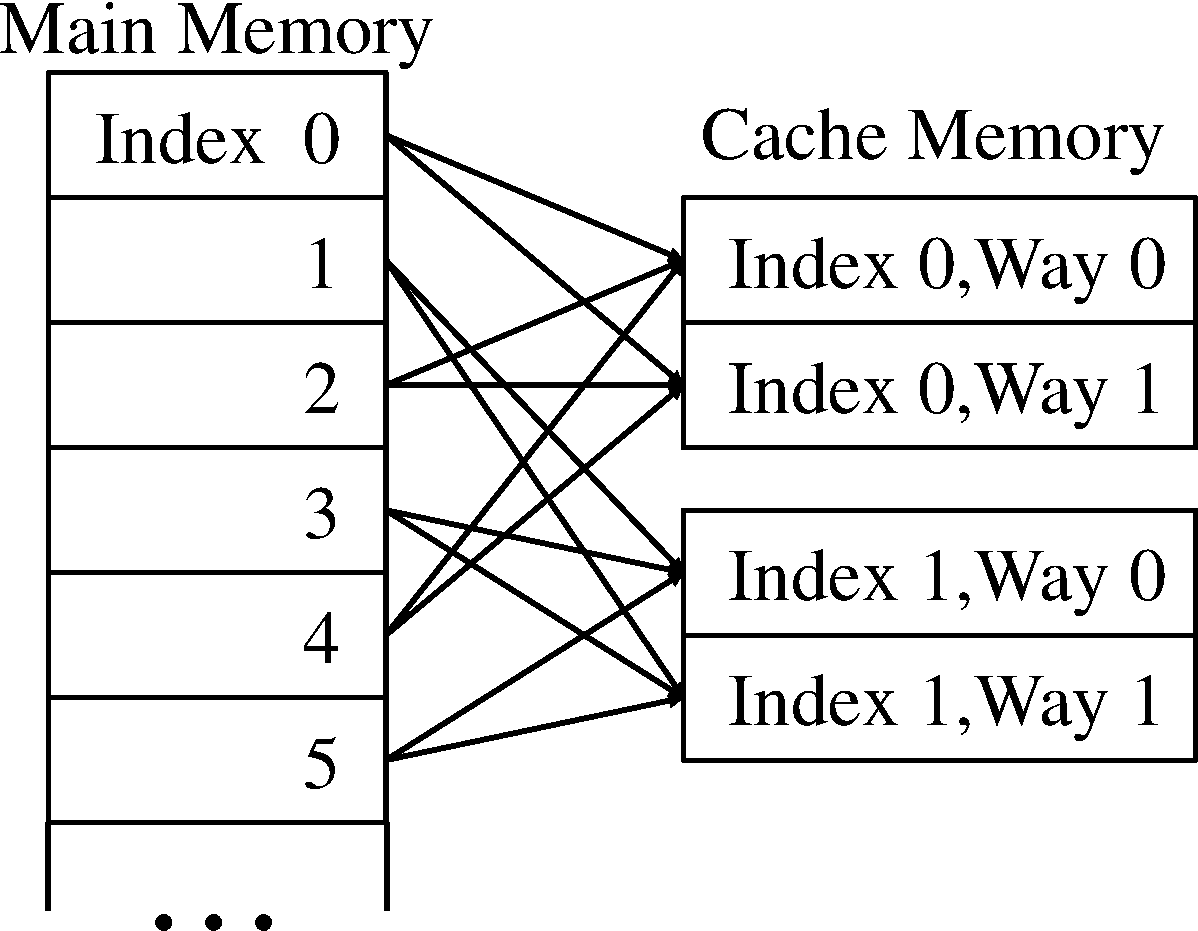
\includegraphics[width=0.32\textwidth]{files/Figures/05-2WayAssoc.pdf}
  }
  \subfloat[Fully Associative]{
     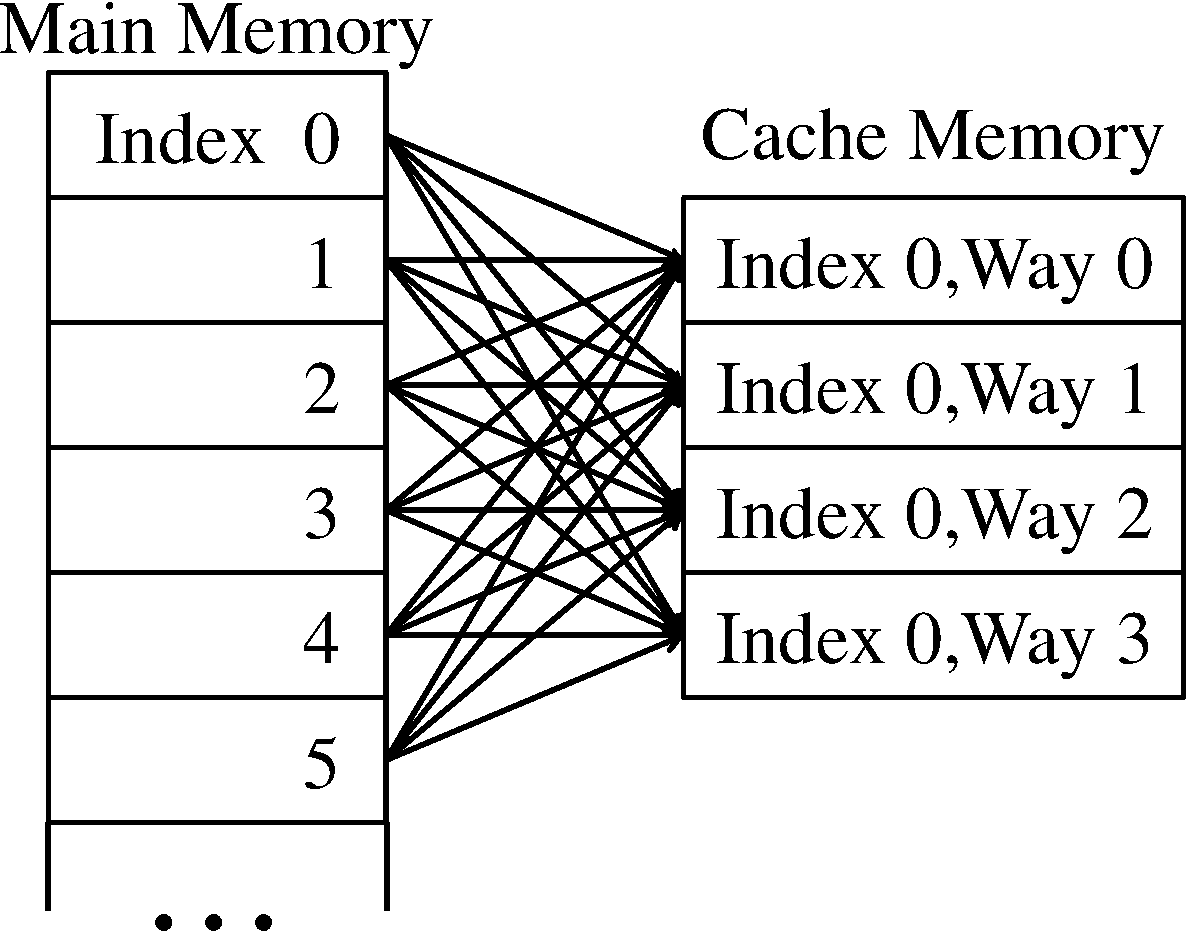
\includegraphics[width=0.32\textwidth]{files/Figures/05-FullAssoc.pdf}
  }
  \caption[Cache Associativity]{ Each block in memory maps to (a) a single entry (way) in the cache (b) one of 2 possible entries (ways) in the cache (c) any entry (way) in the cache}
  \label{fig:cache_associativity}
\end{figure}

\section{Motivation for change}

In conventional caches, the cache block defines the fundamental unit of data
movement and space allocation in caches. The blocks in the data array are
uniformly sized to simplify the insertion / removal of blocks, simplify cache
refill requests, and support low complexity tag organization. Unfortunately,
conventional caches are inflexible (fixed block granularity and fixed \# of
blocks) and caching efficiency is poor for applications that lack high spatial
locality.  Cache blocks influence multiple system metrics including bandwidth,
miss rate, and cache utilization. The block granularity plays a key role in
exploiting spatial locality by effectively prefetching neighboring words all
at once. However, the neighboring words could go unused due to the low
lifespan of a cache block. The unused words occupy interconnect bandwidth and
pollute the cache, which increases the \# of misses. We evaluate the influence
of a fixed granularity block below.

\subsection{Cache Utilization}

In the absence of spatial locality, multi-word cache blocks (typically 64
bytes on existing processors) tend to increase cache pollution and fill the
cache with words unlikely to be used.  To quantify this pollution, we segment
the cache line into words (8 bytes) and track the words touched before the
block is evicted.  We define utilization as the average \# of words touched in
a cache block before it is evicted. We study a comprehensive collection of
workloads from a variety of domains: 6 from PARSEC~\cite{Bienia:2008:PBS:1454115.1454128}, 7 from
SPEC2006, 2 from SPEC2000, 3 Java workloads from DaCapo~\cite{Blackburn:2006:DBJ:1167473.1167488}, 3
commercial workloads (Apache, SpecJBB2005, and TPC-C~\cite{Llanos:2006:TOT:1228268.1228270}), and the
Firefox web browser.  Subsets within benchmark suites were chosen based on
demonstrated miss rates on the fixed granularity cache (i.e., whose working
sets did not fit in the cache size evaluated) and with a spread and diversity
in cache utilization.  We classify the benchmarks into 3 groups
based on the utilization they exhibit: Low ($<$33\%), Moderate (33\%---66\%),
and High (66\%+) utilization (see Table~\ref{table:benchmark_categories}).

\begin{table}[!htb]
\vspace{-10pt}
\begin{center}
\caption{Benchmark Groups}
\label{table:benchmark_categories}
{
  \begin{tabular}{ |@{~}c@{~}|@{~}c@{~}|@{~}p{0.6\columnwidth}@{~}|}
    \hline
    Group & Utilization \% & Benchmarks \\
    \hline
    Low        & 0 --- 33\% & art, soplex, twolf, mcf, canneal, lbm, omnetpp \\
    \hline
    Moderate   & 34 --- 66\% & astar, h2, jbb, apache, x264, firefox, tpc-c, freqmine, fluidanimate \\
    \hline
    High       & 67 --- 100\% & tradesoap, facesim, eclipse, cactus, milc, ferret \\
    \hline
  \end{tabular}
 }
\end{center}
\end{table}
 %% Categories

\begin{figure}[!h]

 \centering
  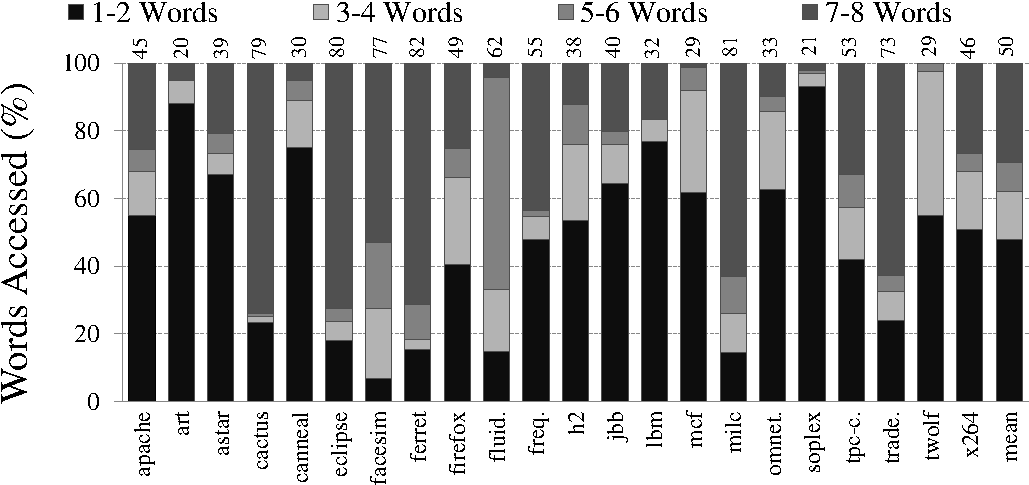
\includegraphics[width=\textwidth]{files/Plots/05-StackBar_Word_Access_64K.pdf}
  \caption[Distribution of words touched]{Distribution of words touched in a cache
    block. Avg. utilization is on top. (Config:
    64K, 4 way, 64-byte block.)}
  \label{fig:stackbar_words_64k}
\end{figure}

Figure~\ref{fig:stackbar_words_64k} shows the histogram of words touched at
the time of eviction in a cache line of a 64K, 4-way cache  (64-byte block, 8
words per block) across the different benchmarks.  Seven applications have
less than 33\% utilization and 12 of them are dominated ($>$50\%) by 1-2 word
accesses.  In applications with good spatial locality (cactus, ferret,
tradesoap, milc, eclipse) more than 50\% of the evicted blocks have 7-8 words
touched. Despite similar average utilization for applications such as astar
and h2 (39\%), their distributions are dissimilar; $\simeq$70\% of the blocks
in astar have 1-2 words accessed at the time of eviction,  whereas
$\simeq$50\% of the blocks in h2 have 1-2 words accessed per block.
Utilization for a single application also changes over time; for example,
ferret's  average utilization, measured as the average fraction of words used
in  evicted cache lines over 50 million instruction windows,  varies from 50\%
to 95\% with a periodicity of roughly 400 million instructions.

%Different temporal phases and 
%memory regions
%within an application may have different requirements: in firefox, 40\% of
%the blocks have 1--2 words touched, 26\% of the blocks have 3--4 words
%touched, and 34\% have 5+ words touched. 
%Overall, the utilization plot
%indicates the need for run time adjustment of cache block granularity.

\subsection{Causes of poor cache utilization}

Applications display poor cache utilization due to inefficient data structure access patterns. This could be due to 
\begin{enumerate}
  \item Programming practices : The array of structs (AoS) approach is a common programming practice. While performing computations upon the array if all elements of the struct are not referenced in close proximity, it could cause poor cache utilisation. A relevant example can be seen in listing \ref{src:bscholes}.
  \item Incorrect assumptions about hardware : Hardware conscious code which attempts to optimise for cache behaviour based on assumptions should be ported carefully. We found \textbf{streamcluster} of the PARSEC application suite, by default, attempt to optimise cache behaviour for 32 byte cache line sizes. This finding was also reported by Liu and Berger\cite{Liu:2011:SPD:2048066.2048070}.
  \item Compiler directives : For better cache performance, sometimes compilers can attempt to allocate aligned blocks of memory. This functionality is exported to the programmer as \code{posix\_memalign} by \textit{GCC}, \code{\_\_aligned\_malloc} by \textit{MSVC} and \code{ippMalloc} by \textit{ICC}. These allocators may leave gaps filled with garbage values which are picked up by the cache when an entire line is fetched, thus reducing the effective caching capacity and reducing utilization.
  \item Interaction with cache geometry : Due to the set associative nature of conventional caches, a set can only contain a fixed number of ways. For instance, if a large amount of data is accessed in a strided fashion which happens to map to the same set, will cause evictions even though there may be space available for use in the other sets of the cache. This shortens the lifetime of the cache blocks in the selected set and may reduce utilization.
\end{enumerate}

\lstset{
  language=C++,
  % keywordstyle=\bfseries\ttfamily\color[rgb]{0,0,1},
  % identifierstyle=\ttfamily,
  % commentstyle=\color[rgb]{0.133,0.545,0.133},
  % stringstyle=\ttfamily\color[rgb]{0.627,0.126,0.941},
  showstringspaces=false,
  basicstyle=\small,
  numberstyle=\footnotesize,
  numbers=left,
  stepnumber=1,
  numbersep=10pt,
  tabsize=4,
  breaklines=true,
  prebreak = \raisebox{0ex}[0ex][0ex]{\ensuremath{\hookleftarrow}},
  breakatwhitespace=false,
  aboveskip={1.5\baselineskip},
  columns=fixed,
  %upquote=true,
  extendedchars=true,
  frame=single,
  frameround=tttt,
  captionpos=b,
  float=tb,
  boxpos=c,
  caption={Code snippet from the initialisation phase of \textbf{blackscholes} benchmark from the PARSEC 2.1 \cite{Bienia:2008:PBS:1454115.1454128} application suite. The code references each \textit{OptionData} structure in the data array where the first 6 fields (24 bytes, as observed on a x86-64 machine with Ubuntu and gcc version 4.4.7) are referenced out of each struct which contains 9 fields (36 bytes). The problem is exacerbated as the \textit{OptionData} structure is allocated as a single chunk and is not cache aligned. The rest of the program demonstrates good cache behaviour.},
  % rulesepcolor=\color{black},
  % backgroundcolor=\color{lbcolor},
}

\noindent\begin{minipage}{\textwidth}
\begin{lstlisting}[label={src:bscholes}]
  /* blackscholes.c:354 */
  for (i=0; i<numOptions; i++) 
  {
      otype[i]      = (data[i].OptionType == 'P') ? 1 : 0;
      sptprice[i]   = data[i].s;
      strike[i]     = data[i].strike;
      rate[i]       = data[i].r;
      volatility[i] = data[i].v;
      otime[i]      = data[i].t;
  }
\end{lstlisting}
\end{minipage}

\begin{figure}[ht]

  \subfloat[64K - Low]{
    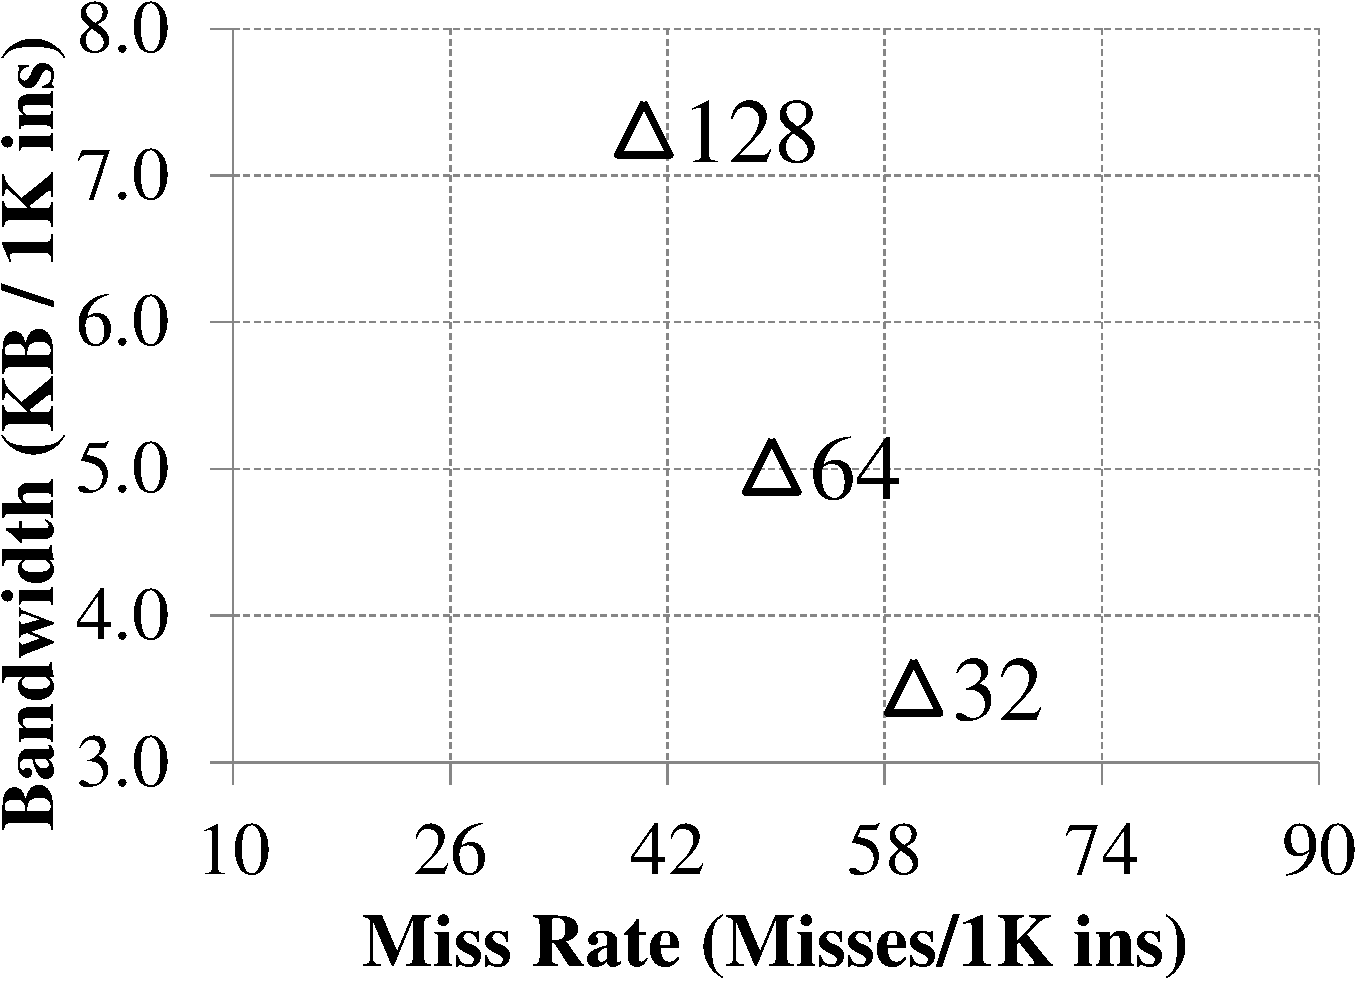
\includegraphics[width=0.48\textwidth]{files/Plots/05-Scatter_Bw_Miss_64K_low.pdf}
  }
  \subfloat[1M - Low]{
     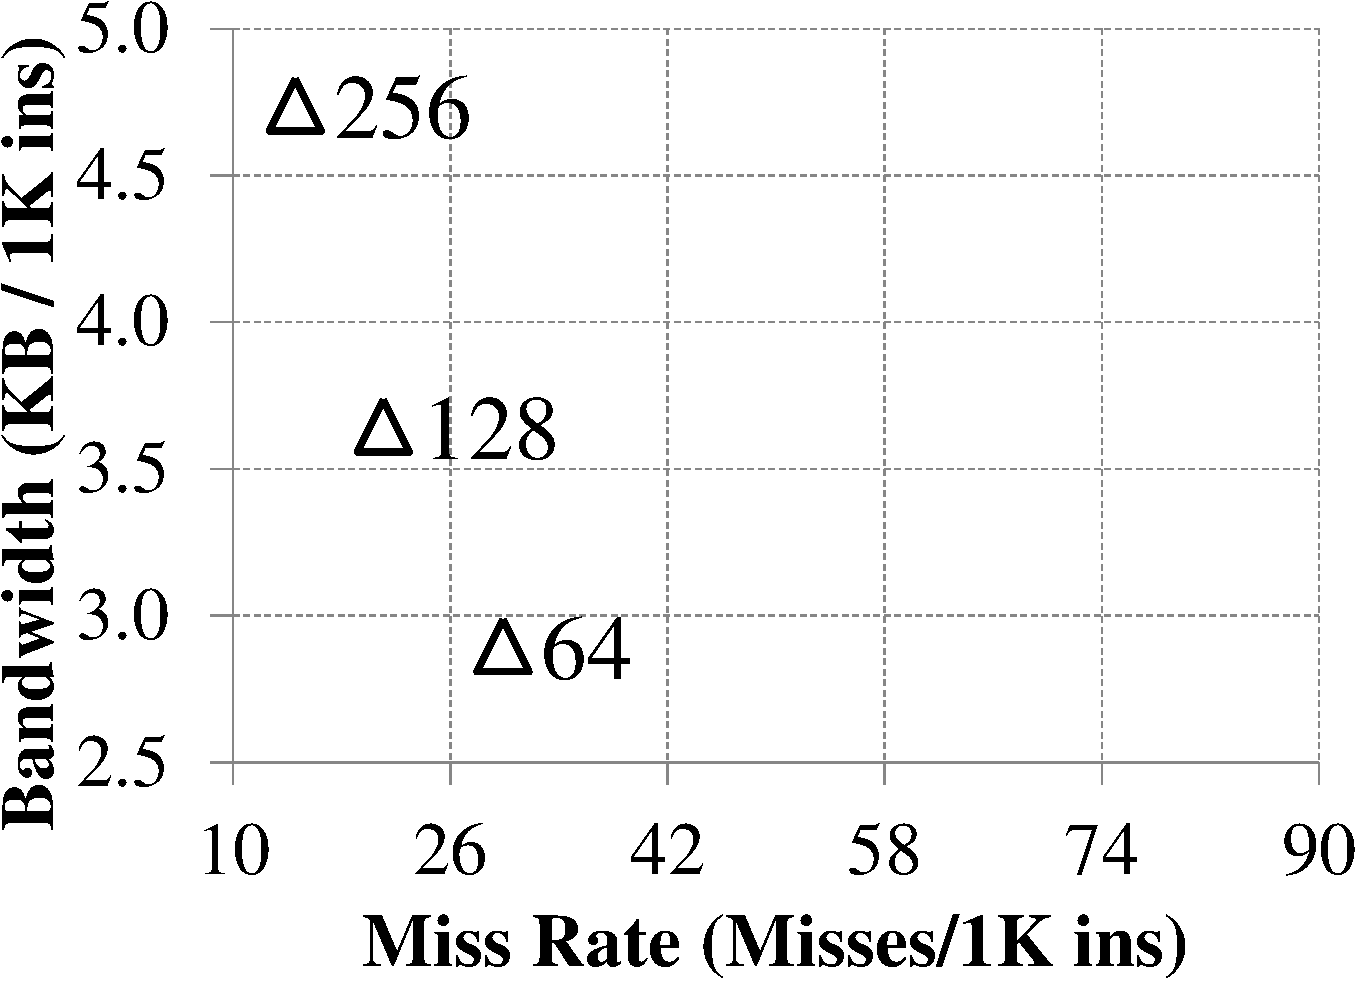
\includegraphics[width=0.48\textwidth]{files/Plots/05-Scatter_Bw_Miss_1M_low.pdf}
  }
  
  \subfloat[64K - Moderate]{
    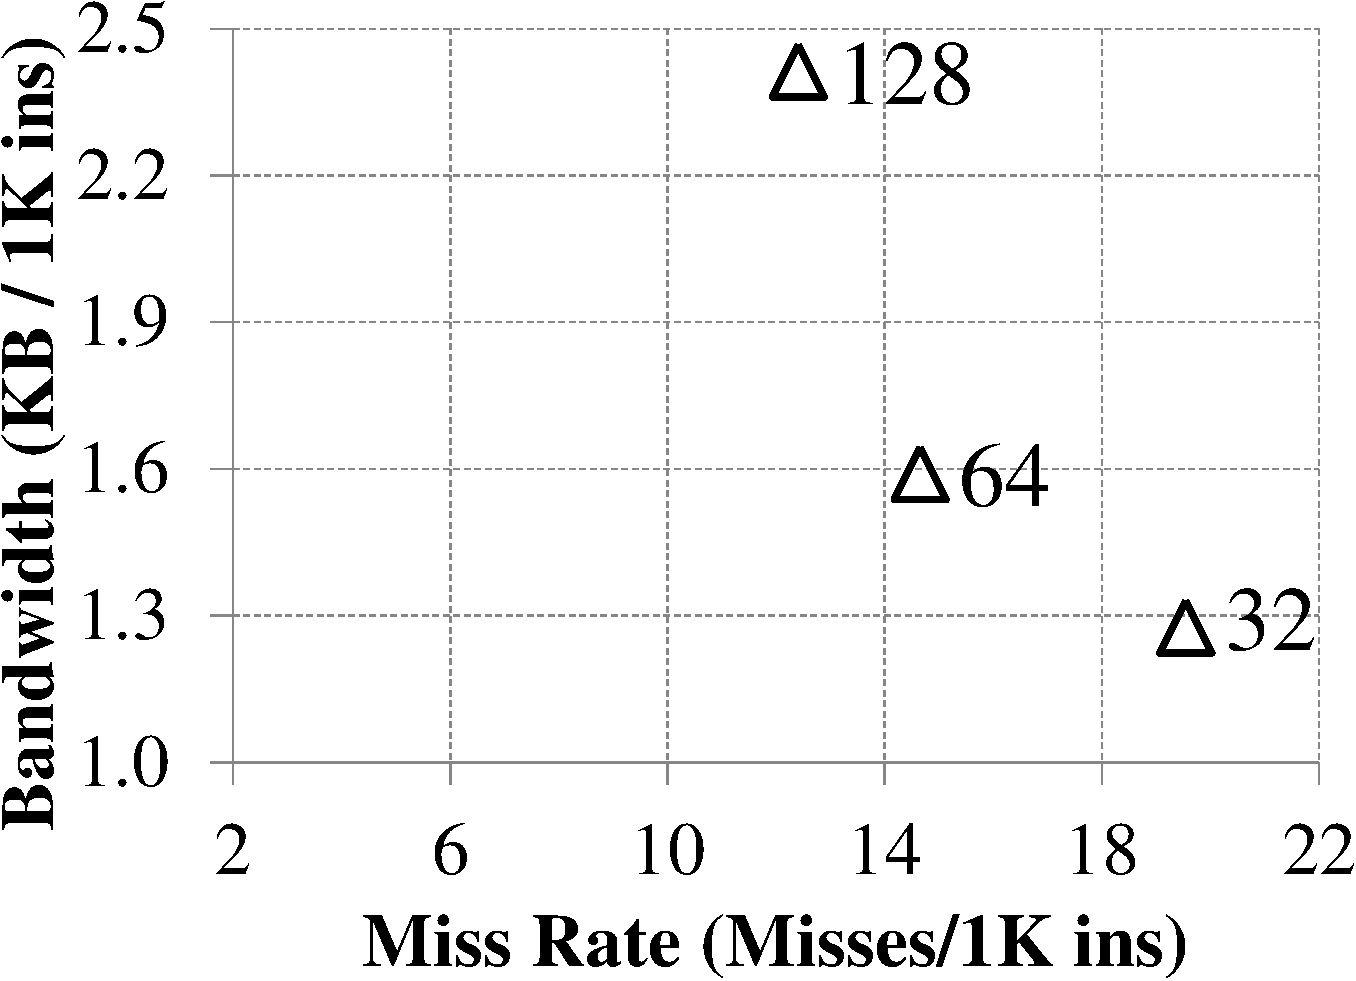
\includegraphics[width=0.48\textwidth]{files/Plots/05-Scatter_Bw_Miss_64K_mod.pdf}
  }
  \subfloat[1M - Moderate]{
     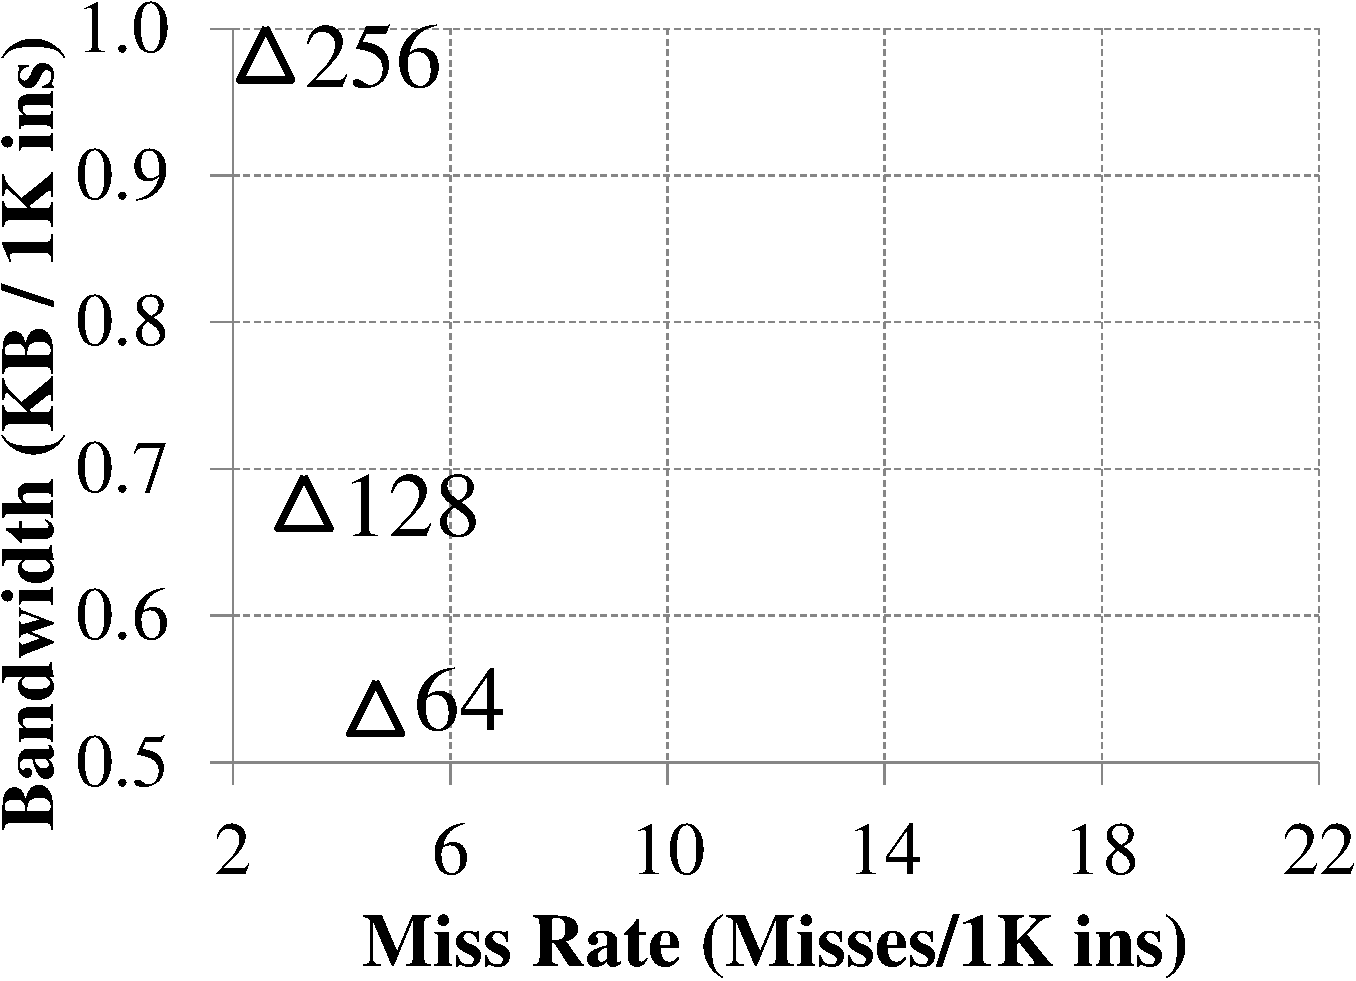
\includegraphics[width=0.48\textwidth]{files/Plots/05-Scatter_Bw_Miss_1M_mod.pdf}
  }
    
  \subfloat[64K - High]{
    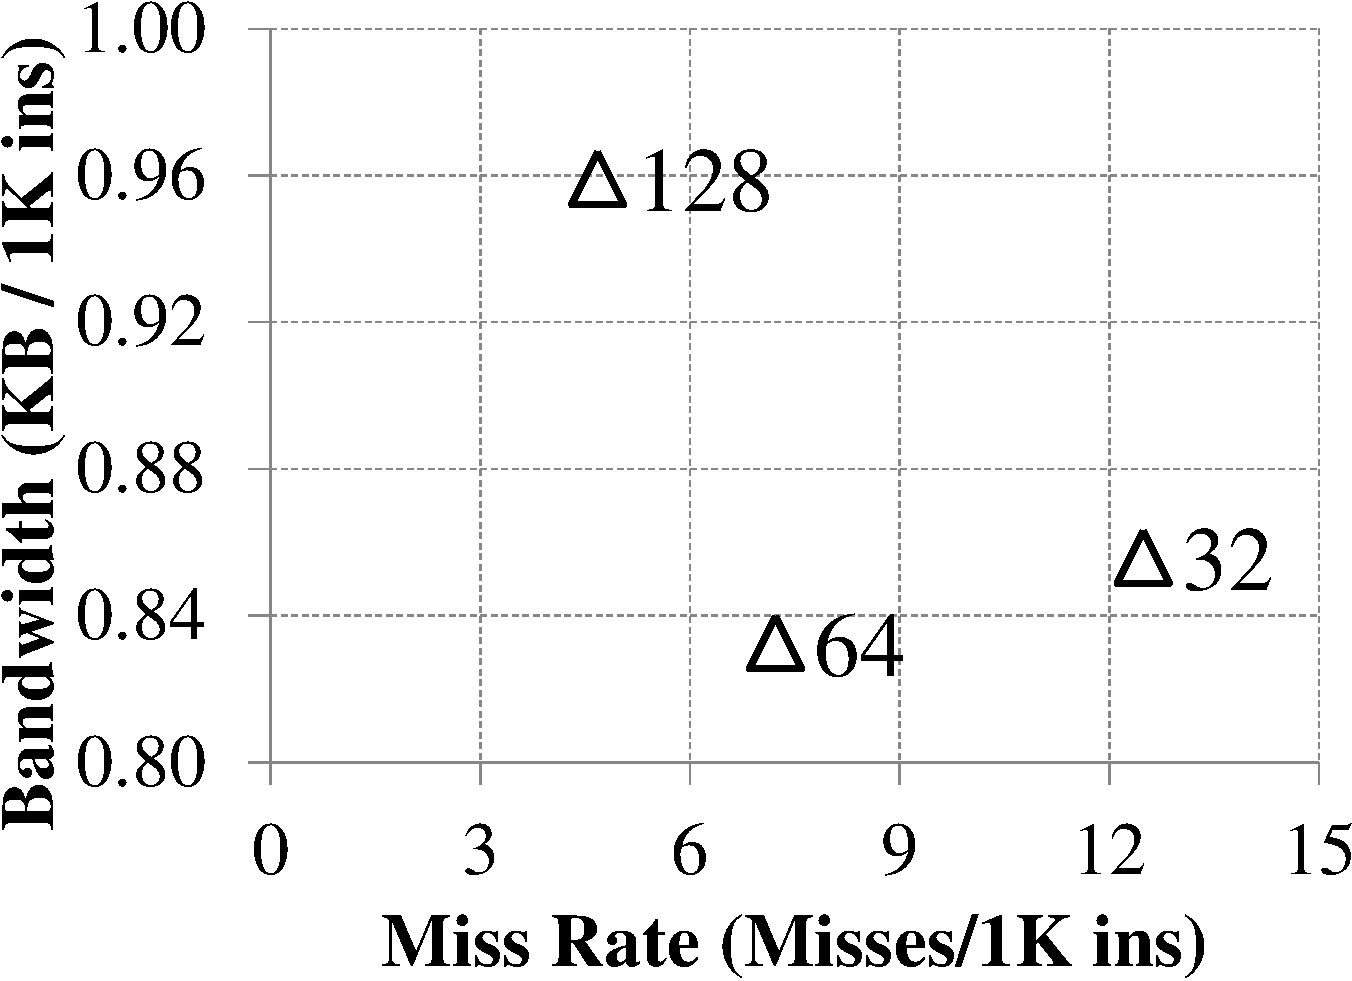
\includegraphics[width=0.48\textwidth]{files/Plots/05-Scatter_Bw_Miss_64K_high.pdf}
  }
  \subfloat[1M - High]{
     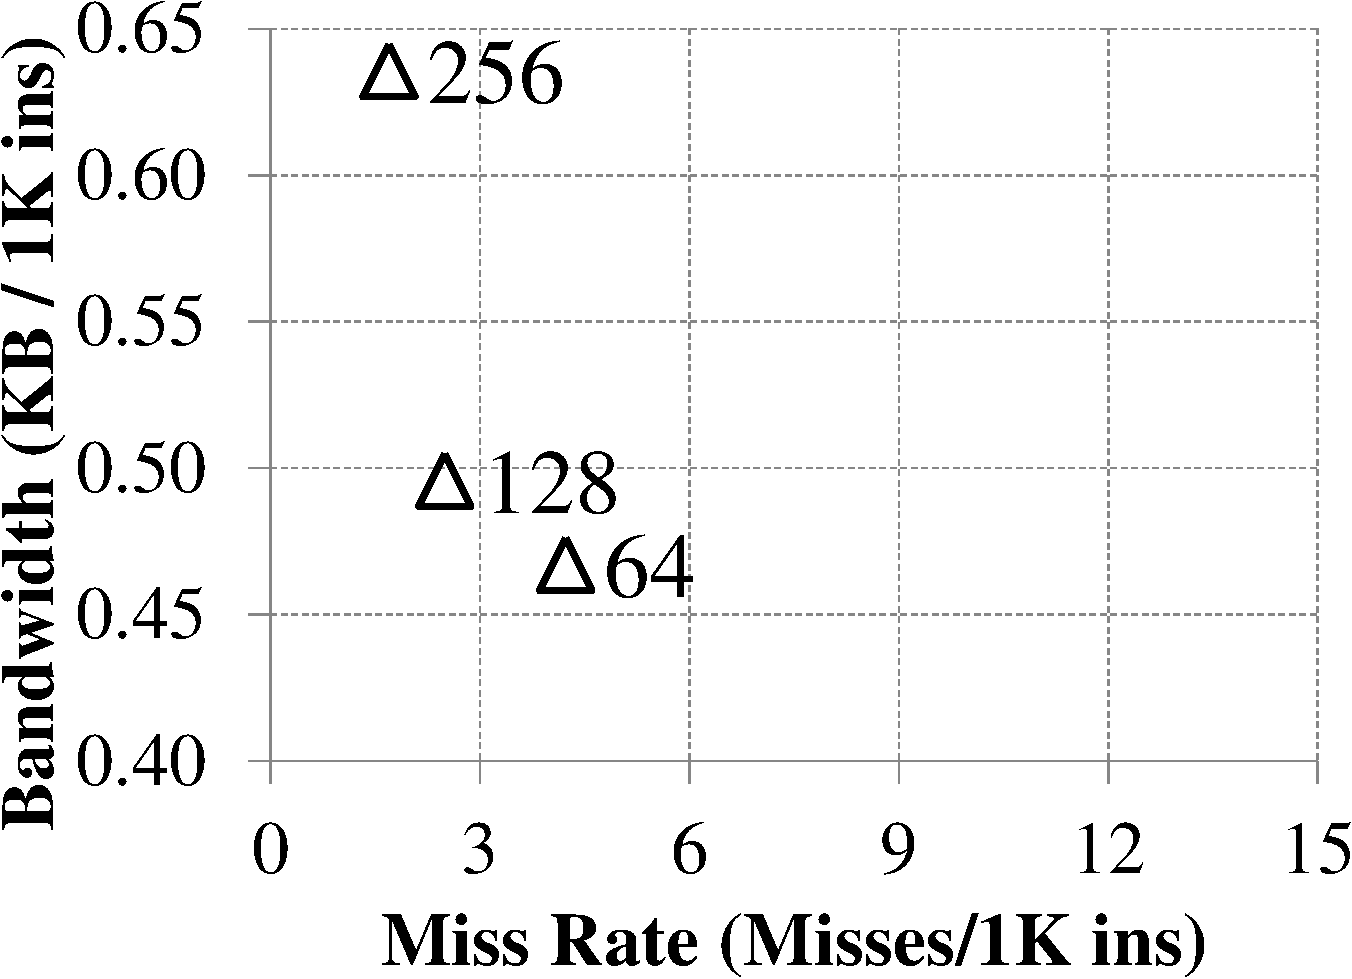
\includegraphics[width=0.48\textwidth]{files/Plots/05-Scatter_Bw_Miss_1M_high.pdf}
  }

  \caption[Bandwidth vs. Miss Rate]{Bandwidth vs. Miss Rate. (a),(c),(e): 64K, 4-way
    L1. (b),(d),(f): 1M, 8-way LLC.  Markers on the plot indicate cache
    block size. Note the different scales for different groups.}
  \label{fig:scatter_bw_64k_1m}
\end{figure}

\clearpage

\subsection{Effect of Block Granularity on Miss Rate and Bandwidth}

Cache miss rate directly correlates with performance, while under
current and future wire-limited technologies, bandwidth
directly correlates with dynamic energy.
Figure~\ref{fig:scatter_bw_64k_1m} shows the influence of block
granularity on miss rate and bandwidth for a 64K L1 cache and a 1M L2
cache keeping the number of ways constant. For the 64K L1, the plots
highlight the pitfalls of simply decreasing the block size to
accommodate the Low group of applications; miss rate increases by
2$\times$ for the High group when the block size is changed from 64B
to 32B; it increases by 30\% for the Moderate group. A smaller block
size decreases bandwidth proportionately but increases miss rate. With
a 1M L2 cache, the lifetime of the cache lines increases significantly, 
improving overall utilization. Increasing the block size from
64$\to$256 halves the miss rate for all application groups. 
The bandwidth is increased by 2$\times$ for the Low and Moderate.


\begin{table}[!h]
\caption{Optimal block size. Metric: $\mathbf{\frac{1}{Miss-rate \times Bandwidth}}$}
\label{table:bwmr_classify}
\begin{center}
{
\small
  \begin{tabular}{ |@{~}c@{~}| m{0.72\columnwidth} |}
    \hline
    \multicolumn{2}{|c|}{64K, 4-way} \\
    \hline
    Block  & Benchmarks \\
    \hline
    32B   & cactus, eclipse, facesim, ferret, firefox, fluidanimate,freqmine, milc, tpc-c, tradesoap \\
    \hline
    64B   &  art \\
    \hline
    128B  & apache, astar, canneal, h2, jbb, lbm, mcf, omnetpp, soplex, twolf, x264 \\
    \hline
    \multicolumn{2}{|c|}{1M, 8-way} \\
    \hline
    Block & Benchmarks \\
    \hline
    64B  & apache, astar, cactus, eclipse, facesim, ferret, firefox, freqmine, h2, lbm, milc, omnetpp, tradesoap, x264\\
    \hline
    128B & art\\
    \hline
    256B  & canneal, fluidanimate, jbb, mcf, soplex, tpc-c, twolf\\
    \hline
  \end{tabular}
}
\end{center}
\end{table}




Since miss rate and bandwidth have different optimal block
granularities, we use the following metric: $\frac{1}{Miss Rate \times
  Bandwidth}$ to determine a fixed block granularity suited to an
application that takes both criteria into account.
Table~\ref{table:bwmr_classify} shows the block size that maximizes
the metric for each application.  It can be seen that different
applications have different block granularity requirements.  For
example, the metric is maximized for apache at 128 bytes and for
firefox (similar utilization) at 32 bytes.  Furthermore, the optimal
block sizes vary with the cache size as the cache lifespan
changes. This highlights the challenge of picking a single block size
at design time especially when the working set does not fit in the
cache.
%In short, \textit{the tradeoff between increasing the 
%  cache block granularity to achieve spatial prefetching and lower miss rate, 
%  and reducing the granularity to minimize traffic and pollution needs
%  adaptive cache blocks.}

\subsection{Need for adaptive cache blocks}
Our observations motivate the need for adaptive cache line
granularities that match the spatial locality of the data access patterns
in an application. In summary:
\begin{itemize}
  \item  Smaller cache lines improve utilization but tend to increase
    miss rate and potentially traffic for applications with good
    spatial locality, affecting the overall performance.
  \item Large cache lines pollute the cache space and interconnect
    with unused words for applications with poor spatial locality, 
   significantly decreasing the caching efficiency.
  \item Many applications waste a significant fraction of the cache
  space. Spatial locality varies not only across applications but also
  within each application, for different data structures as well as 
  different phases of access over time.   

%\item Optimizing miss rate (impacts performance), bandwidth (impacts
%  dynamic energy), and utilization simultaneously with a fixed size
%  cache line is not tractable, since in many cases the optimality is
%  achieved at different block sizes.
\end{itemize}


\section{Dissertation Outline}

Chapter \ref{chap:ac_architecture} describes the \AC\ architecture whilst comparing it with conventional architecture and looking at related work. The hardware complexity, implementation issues and simulator infrastructure are discussed in Chapter \ref{chap:hardware_complexity_and_simulation}. The experimental results of an exhaustive evaluation of the \AC\ is presented in Chapter \ref{chap:evaluation}. Conclusions and future work are outlined in Chapter \ref{chap:conclusions}.
 
%!TEX root=/home/ska124/Dropbox/Thesis/thes-full.tex
%%%%%%%%%%%%%%%%%%%%%%%%%%%%%%%%%%%%%%%%%%%%%%%%%%%%
%
%     Chapter 3   
%
%%%%%%%%%%%%%%%%%%%%%%%%%%%%%%%%%%%%%%%%%%%%%%%%%

\chapter{Amoeba Cache Architecture}
\label{chap:ac_architecture}

As described in \S~\ref{sec:cache_memory_systems}, a conventional cache organises the data array into a 2 dimensional structure. A transparently addressed cache uses the same namespace (memory address space layout) as the main memory. The blocks which are stored in the sets are \textit{tagged} with the aligned start address of block present in the main memory. The \textit{tags} for the cache blocks currently present in the cache set are maintained in a separate array. When a search is being performed to find out whether a required physical address is present in the cache, the tag array is looked up to determine a cache hit or a cache miss. The organization of the cache set and tag array is shown in Figure \ref{fig:set_assoc_arch}. The effective address is the virtual address supplied by the CPU of the required datum. The component bits of the effective address is segmented into 3 parts which form the \textit{Virtual Page Number(VPN)}, set number and byte offset. The set number and byte offset are looked up in the tag array while the VPN is looked up in the \textit{Translation Lookaside Buffer(TLB)} to check that the current process has brought in the corresponding page and it is valid. The organisation described (and shown in Fig \ref{fig:set_assoc_arch}) is virtually indexed, physically tagged organisation where the lookup logic does not include the TLB translation in the critical path to enable faster searches. There are other organisations such as virtually indexed, virtually tagged and physically indexed, physically tagged which are uncommon due to inherent issues with their design. The tradeoff for a virtually indexed, physically tagged cache is that it can only grow in size with an increase in the associativity of each set, or an increase in the size of each cache block. The Intel Sandy Bridge architecture is known to use a virtually indexed, physically tagged cache organisation.



\begin{figure}[b]
  %% Pg 84 - Jacob
  \begin{center}
    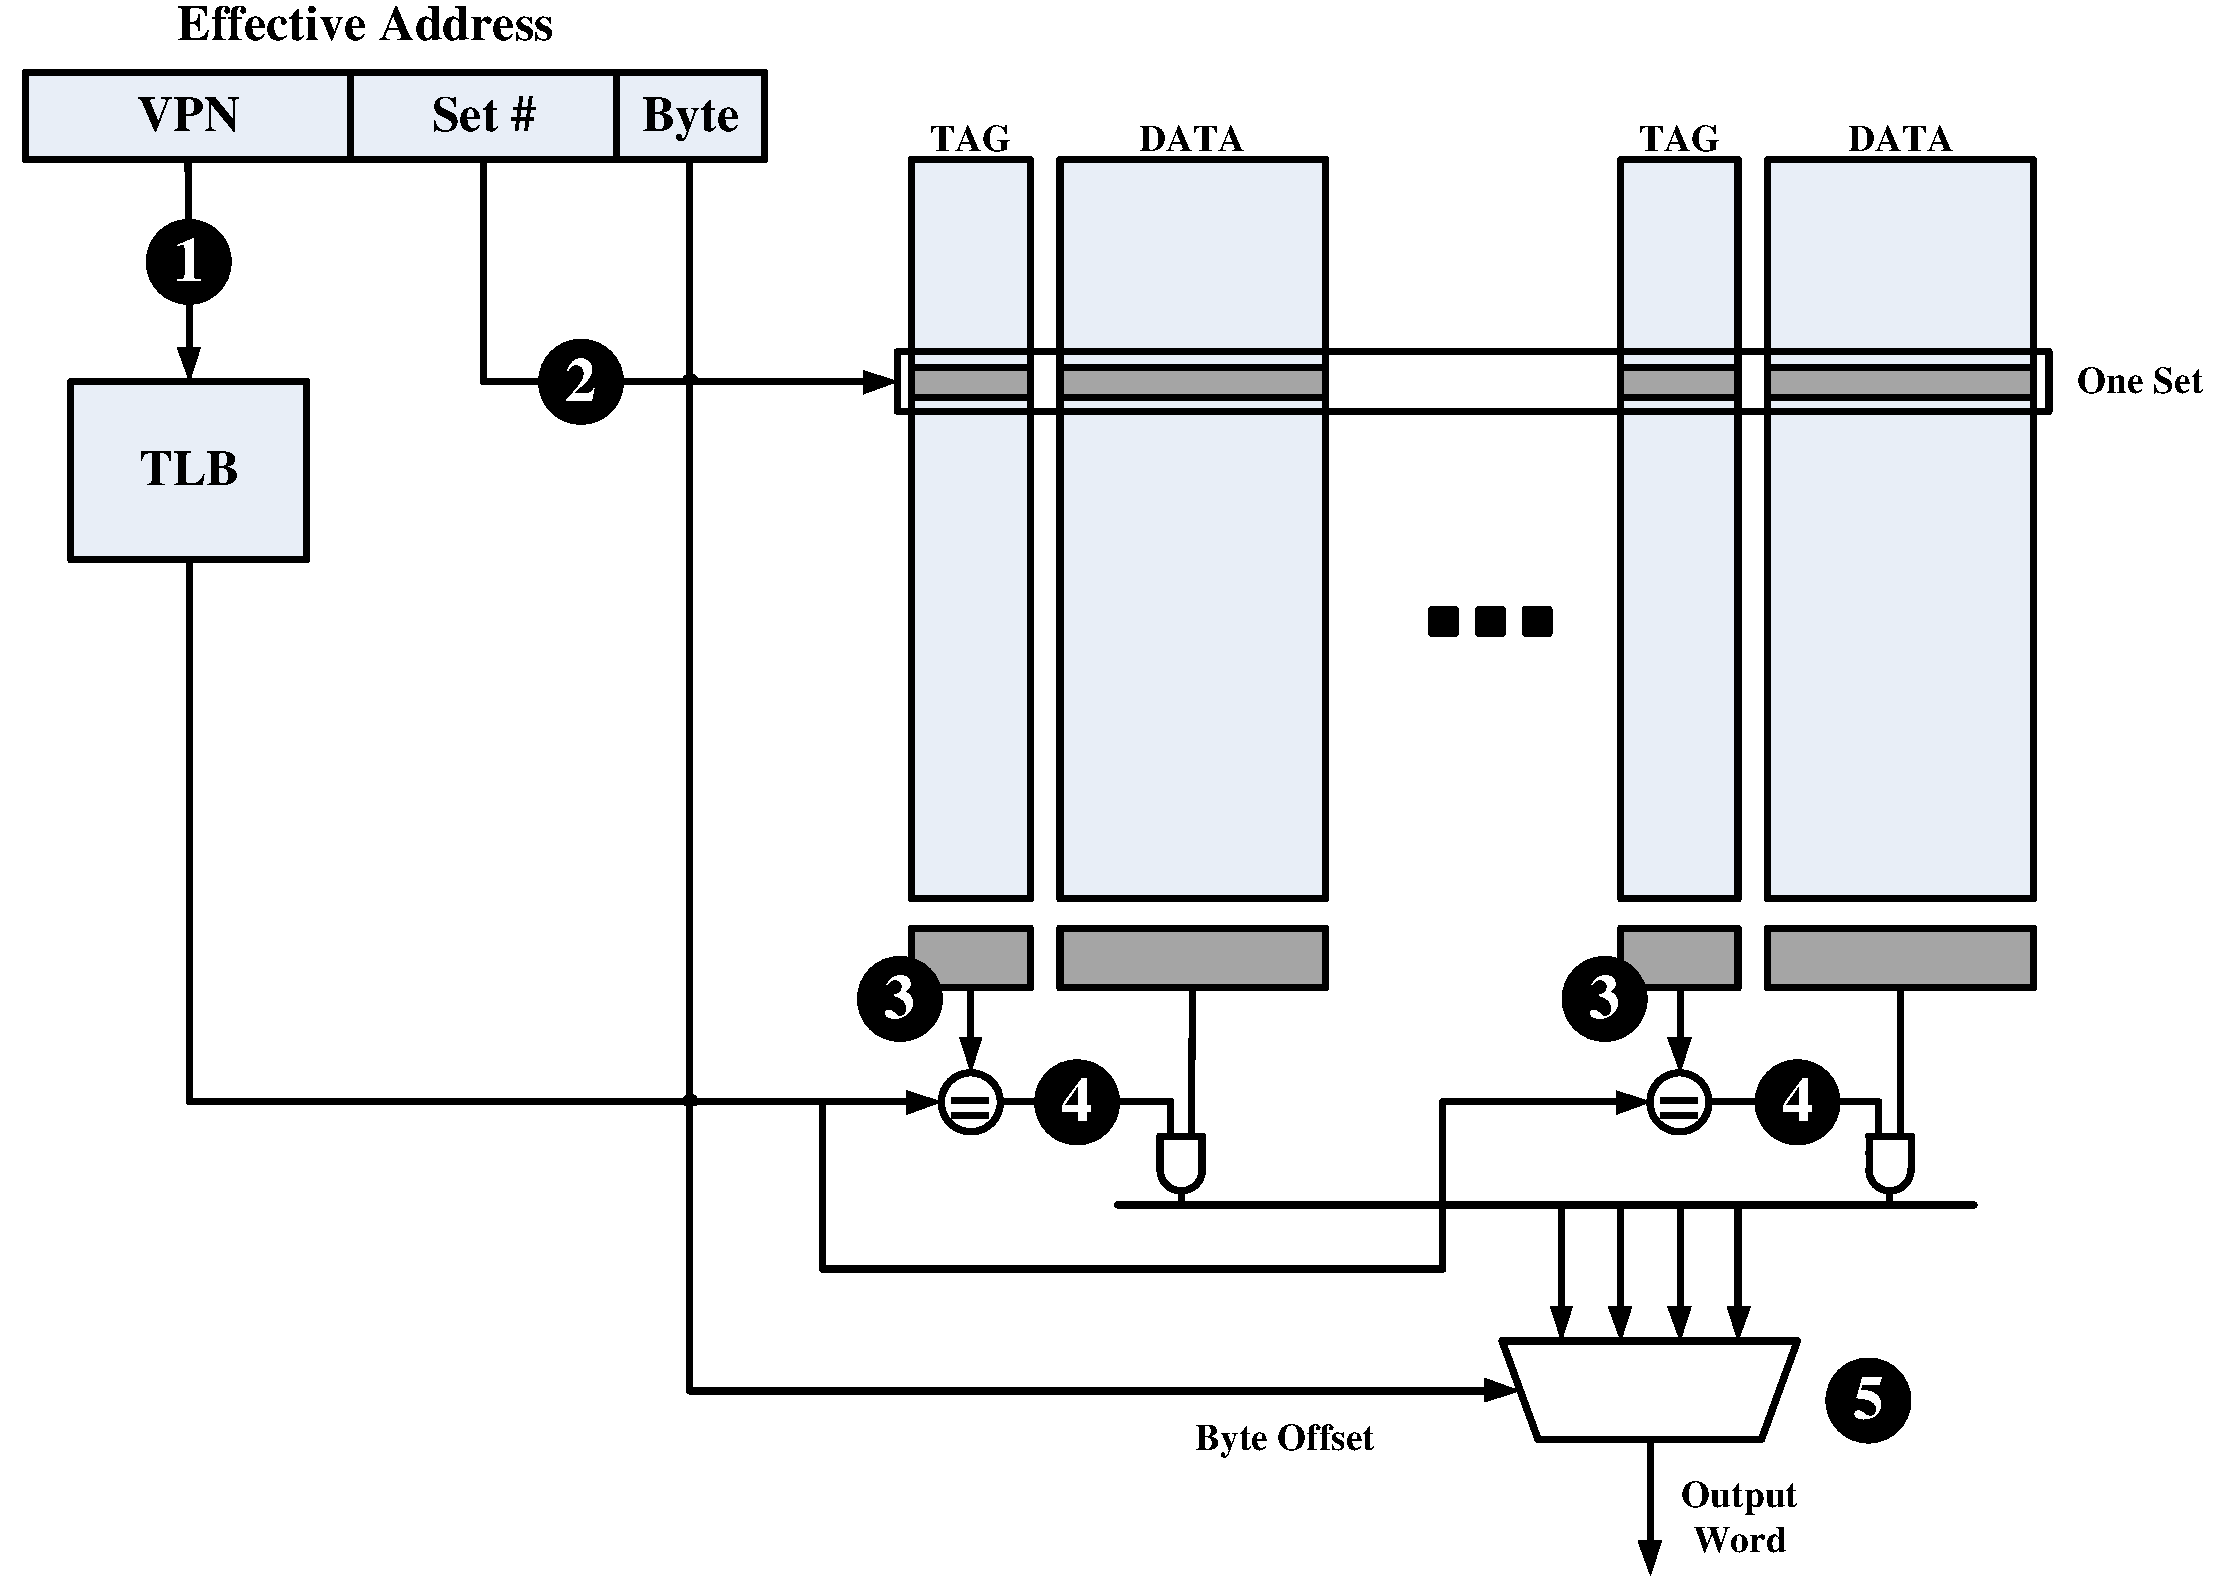
\includegraphics[width=\textwidth]{files/Figures/06-NWaySetAssocCache.pdf}
    \caption[Conventional N-Way Set-Associative Cache]{\textbf{Conventional N-Way Set-Associative Cache} \bigspot{1} The Virtual Page Number (VPN) is used to look up the entry in the Translation Lookaside Buffer (TLB) \bigspot{2} According to the number of sets in the cache, the following bits from the address are used to look up the corresponding set from the cache \bigspot{3} The tags read out from the set are compared with the translation from the TLB and tested for equality \bigspot{4} The corresponding cache block is forwarded to the output buffer for the tag which matches the TLB lookup \bigspot{5} Using the byte offset from the CPU, the mutiplexer selects the correponding critical word }
    \label{fig:set_assoc_arch}
  \end{center}
\end{figure}

\clearpage

In contrast to a conventional cache, the \AC\ architecture enables the memory hierarchy to fetch and allocate space for a range of words (i.e. a variable granularity cache block) based on the spatial locality of the application. For example, consider a 64K cache (256 sets) that allocates 256 bytes per set. These 256 bytes can adapt to support, for example, eight 32-bytes blocks, thirty-two 8-byte blocks, or four 32-byte blocks and sixteen 8-byte blocks, based on the set of contiguous words likely to be accessed. 
\\ \\
The key challenges to realising the \AC\ architecture are
\begin{enumerate}[noitemsep]
	\item To support a variable number of blocks per set
	\item To support a variable granularity for each block
	\item To support a variable number of tags, which correspond to the blocks in the set
\end{enumerate}

\begin{figure}[h]
  \begin{center}
    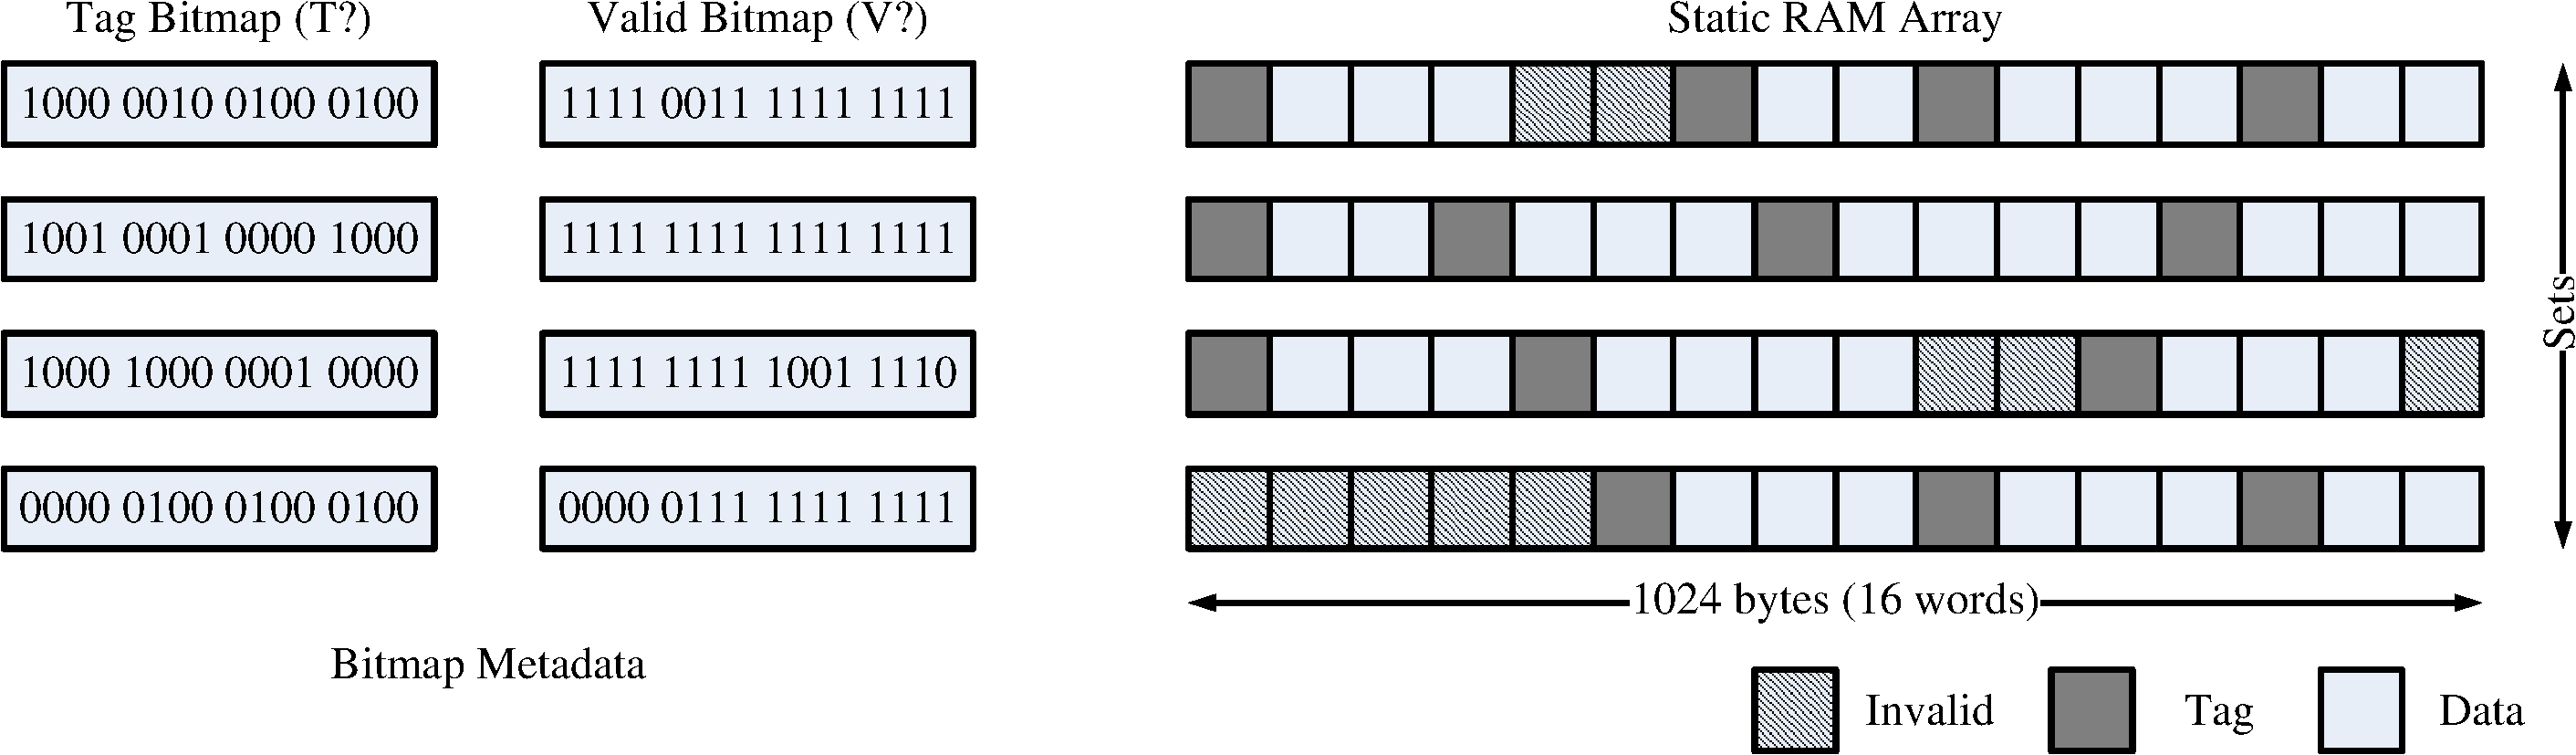
\includegraphics[width=\textwidth]{files/Figures/06-AmoebaCacheArch.pdf}
    \caption[Amoeba Cache Overview]{\textbf{Amoeba Cache Overview} The static RAM (SRAM) array where the tags and data are colocated is shown on the right. The \code{T? Bitmap} and the \code{V? Bitmap} for the \AC\ are shown on the left. Each block in the SRAM array represents 8 bytes (1 word). In this specific example, an \AC\ is shown with 4 sets and 1024 bytes per set. The invalid, data and tag words (marked in the SRAM array) are tracked by setting the corresponding bits in the \code{T? and V? Bitmaps}. This information is maintained in order to simplify cache operations such as insertion and refill. }
    \label{fig:amoeba_cache_arch}
  \end{center}
\end{figure}

The \AC\ adopts a solution inspired by software data structures, where programs hold meta-data and actual data entries in the same address space. To achieve maximum flexibility, the \AC\ completely eliminates the tag array and collocates the tags with the actual data blocks (see Figure~\ref{fig:amoeba_cache_arch}). To distinguish which words are data words and which ones are tags within the set, a bitmap data structure is used (labeled \code{T? Bitmap} in Fig~\ref{fig:amoeba_cache_arch}). For each word in the set which is a tag, the corresponding bit in the \code{T? Bitmap} is set. The conventional valid/invalid bits are also decoupled (typically associated with the tags) and organized into a separate array (labeled \code{V? Bitmap} in Fig~\ref{fig:amoeba_cache_arch}) to simplify block replacement and insertion. \AC\ tags are composed of a \code{Region Tag} and a tuple which consists of the \code{Start} and \code{End} address of the variable granularity cache block. The data block immediately follows the tag word as shown in Fig~\ref{fig:amoeba_cache_arch}. The following sections provide more detail about the \AC\ architecture and how cache operations are performed.


\section{Amoeba Blocks and Set-Indexing}
\label{sec:amoeba_blocks_and_set_indexing}

\begin{figure}[h]
  %% Get images from http://en.wikipedia.org/wiki/CPU_cache#Associativity
  \subfloat[Memory Regions]{
    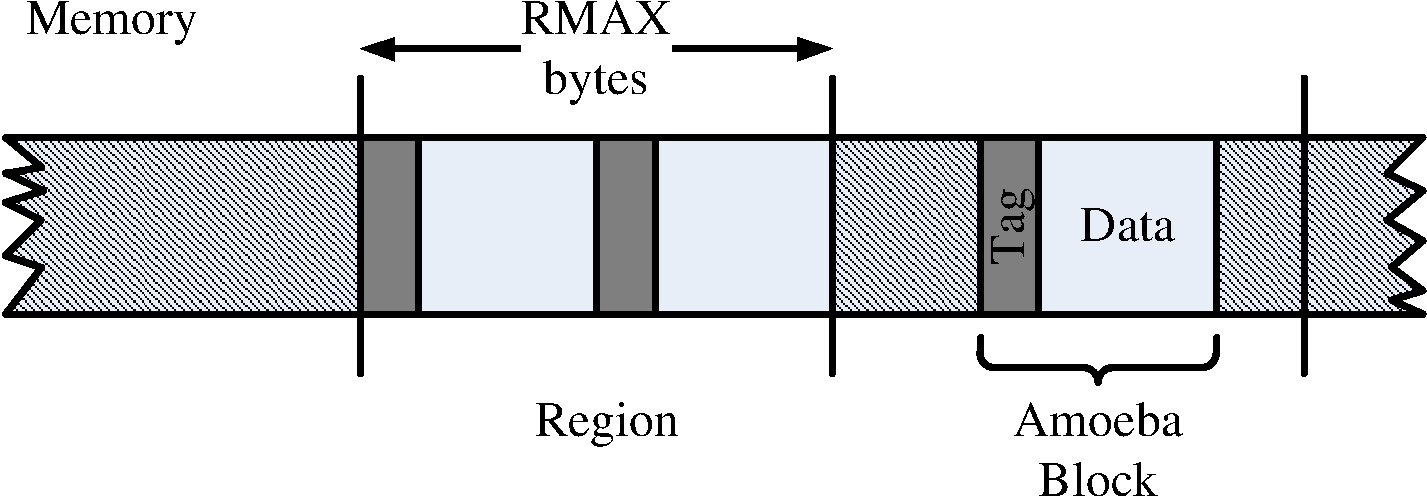
\includegraphics[width=0.5\textwidth]{files/Figures/06-MemoryRegions.pdf}
  }
  \subfloat[Addressing]{
     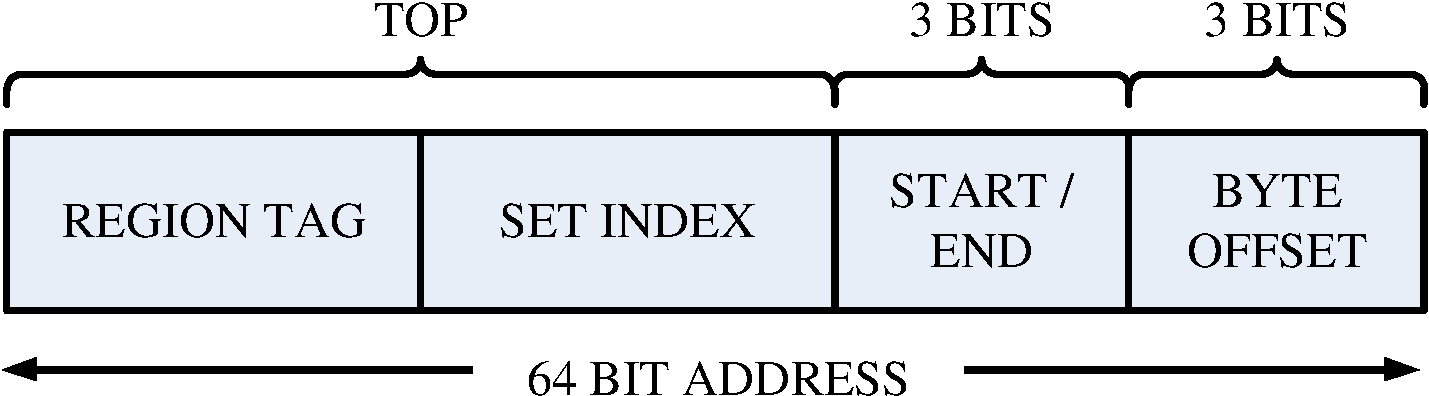
\includegraphics[width=0.5\textwidth]{files/Figures/06-Addressing.pdf}
  }
  \caption[Memory Regions]{ (a) The linear memory address space is segmented into Regions. The \AB{}s are constrainted to have their start and end within a single memory region. (b) 64 bits are used to encode the Region Tag, the Set Index, the start or end word and the word offset in the tag for an \AB{}.  }
  \label{fig:mem_region_addr}
\end{figure}


The \AC\ data array holds a collection of varied granularity \AB{}s that do not overlap. Each \AB\ is a 4 tuple consisting of \code{\textless RegionTag, Start, End, Data-Block\textgreater} (Figure~\ref{fig:amoeba_cache_arch}). The first 3 components of the tuple are equivalent to a tag in a conventional cache. 8 bytes are allocated (1 word) for each tag. In order to simplify cache lookups for \AB{}s, the address space is partitioned into \code{Regions}. A \code{Region} is an aligned block of memory of size \code{RMAX} bytes. The boundaries of any \AB{} block (\code{Start} and \code{End}) are constrained to lie within the regions' boundaries. The minimum granularity of the data in an \AB\ is 1 word and the maximum is \code{RMAX} words. The \code{Start} and \code{End} can be encoded in $log_2(RMAX)$ bits. The set indexing function masks the lower $log_2(RMAX)$ bits to ensure that all \AB{}s (every memory word) from a region index to the same set. The Region Tag and Set-Index are identical for every word in the \AB{}. Retaining the notion of \textit{sets} enables fast lookups and helps elude challenges such as synonyms (same memory word mapping to different sets). When comparing against a conventional cache, \code{RMAX} is set to 8 words (64 bytes), ensuring that the set indexing function is identical to that in the conventional cache to allow for a fair evaluation.



\section{Data Lookup}

When data is referenced by the CPU, a cache lookup takes place in order to determine whether the required datum is present in the cache or not (resulting in a cache hit or miss). The operation percolates down the memory hierarchy until a cache returns a hit or the backing store supplies the datum required. Fig~\ref{fig:set_assoc_arch} shows a conventional cache which operates in \textit{Fast Mode}, where the contents of the entire set is read out into the output buffer in parallel with the tag lookup. Megabyte sized caches, with larger sets, may want to avoid the extra cost of reading out all ways to the output buffer and wait until the tag lookup completes to read out only the required way from the set over the H-tree (for more details see \S~\ref{sec:area_latency_energy_overhead}). Though this saves energy, it serializes the lookup and takes longer. The delay is usually tolerated as the \textit{Serial Mode} lookup is often implemented in the L2 caches or lower in the memory heirarchy. Another approach which minimises energy whilst still reading out the way in parallel is \textit{way prediction}\cite{patent:DataCacheWayPrediction,patent:WayPredictionVirtualHint}, commonly used in processors manufactured by MIPS.

In contrast to a conventional cache, the \AC\ needs to lookup tags from the SRAM array to determine a hit or miss. The metadata stored in the \code{T? Bitmap} is used during the lookup operation in the \AC{}. Figure~\ref{fig:ac_lookup} describes the steps of the lookup procedure in an \AC{}. The overheads incurred due to the extra stages introduced in the critical path are evaluated in chapter \ref{sec:hardware_complexity}.


\begin{figure}[h]
  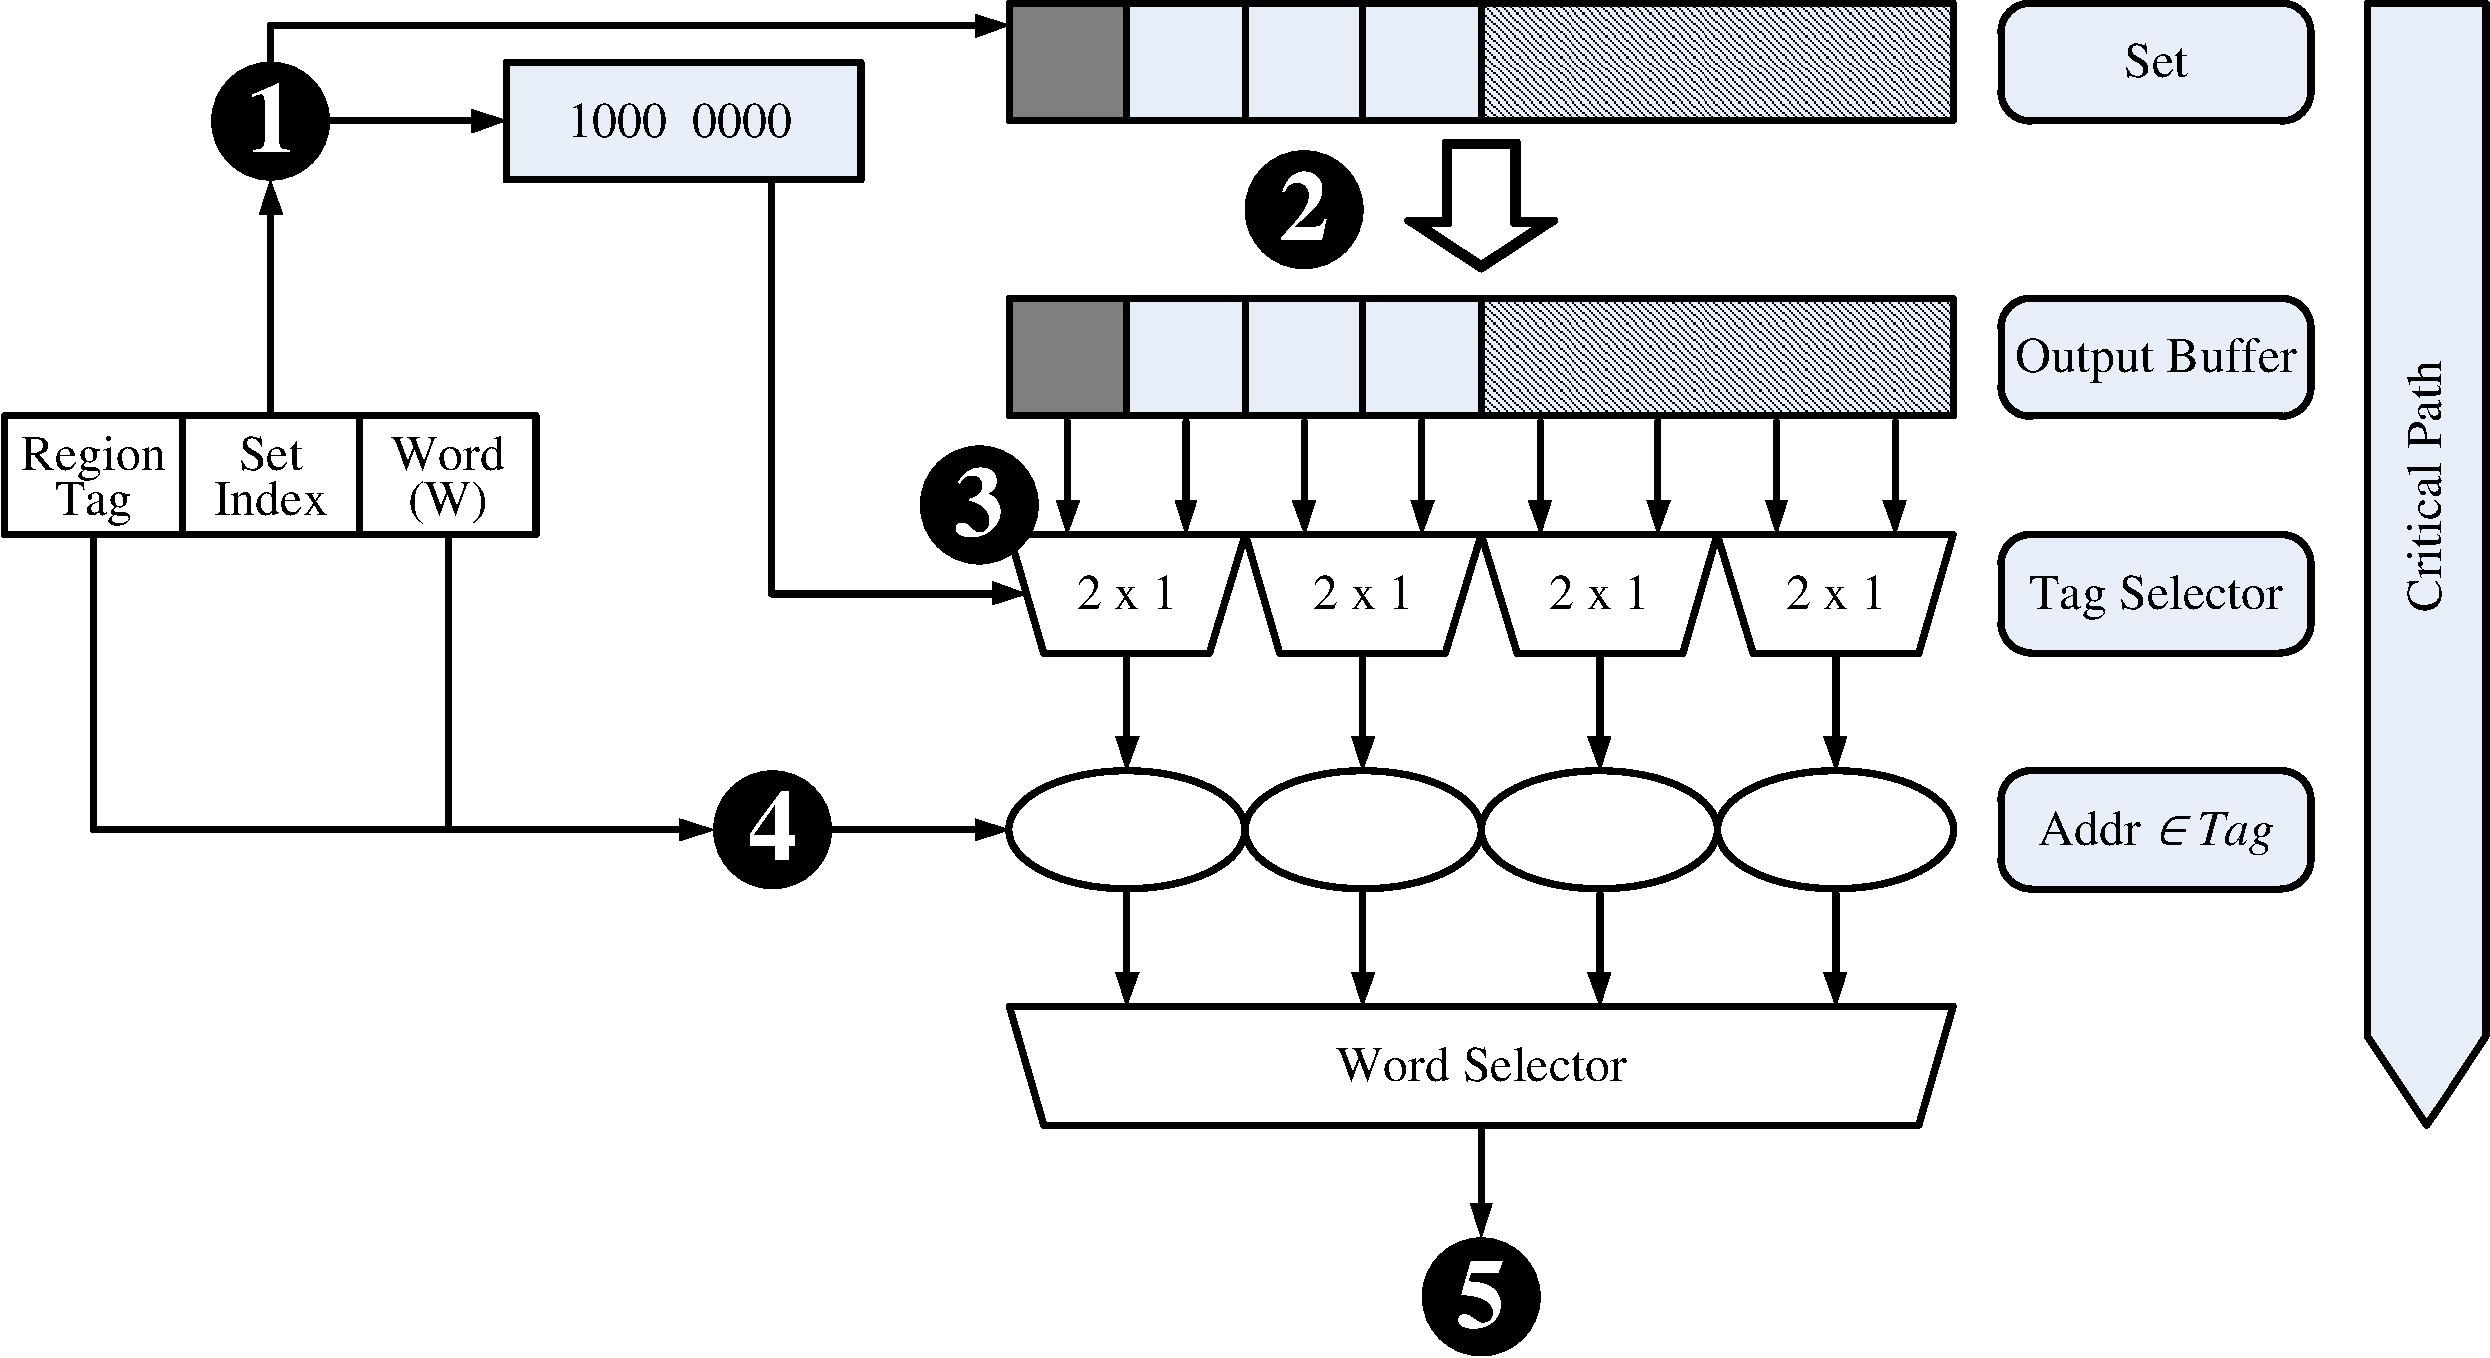
\includegraphics[width=\textwidth]{files/Figures/06-Lookup.pdf}
  \caption[Amoeba Cache Lookup]{\textbf{Amoeba Cache Lookup} : The incoming effective address is segmented into the region tag, set index and word offset. \bigspot{1} The \code{Tag? Bitmap} is looked up to determine which words in the activated set are required for the tag comparison. Note that given the minimum size of a \AB{} is two words (1 word for the tag metadata, 1 word for the data), adjacent words cannot be tags. Given this constraint, 
  the number of 2-1 multiplexers required to route one of the adjacent words to the comparator ($\in$ operator), is equal to half the number of words in the set. \bigspot{2} Simultaneously, the set is activated and the contents are latched onto the output buffer. \bigspot{3} The appropriate tag words are selected with the input from the the \code{Tag? Bitmap}. \bigspot{4} The comparator generates the hit signal for the word selector. The $\in$ operator consists of two comparators: a) an aligned \code{Region tag} comparator, a conventional $==$ (64 - $log_2N_{sets}$ - $log_2{RMAX}$ bits wide, e.g., 50 bits) that checks if the \AB{} belongs to the same region and b) a $ Start <= W < END $ range comparator ($log_2RMAX$ bits wide; e.g., 3 bits) that checks if the \AB\ holds the required word. Finally, in \bigspot{5}, the tag match activates and selects the appropriate word. The critical path (as indicated on the left) includes the read out from the set, the tag selectors and the $\in$ operation.}
  \label{fig:ac_lookup}
\end{figure}

\clearpage

\section{Block Insertion}

On a miss for the desired word, a spatial granularity predictor is invoked (see \S~\ref{sec:spatial_pattern_predictor}), which specifies the range of the \AB{} to refill. To determine a position in the set to slot the incoming block use the information contained in the \code{Valid? Bitmap}. The \code{V? Bitmap} has 1 bit/word in the cache; a ``1'' bit indicates the word has been allocated (valid data or a tag). To find space for an incoming data block, a substring search is performed on the \code{V? Bitmap} of the cache set for contiguous 0s (empty words). For example, to insert an \AB{} of five words (four words for data and one word for tag), a substring search is performed for \textit{00000} in the \code{V? Bitmap} / set (e.g., 32 bits wide for a 64K cache). If the required amount of space is not found, the replacement algorithm is repeatedly triggered until the required amount of contiguous space is found. Following this, the \AB\ tuple (Tag and Data block) is inserted, and the corresponding bits in the \code{T? and V? Bitmaps} are set. The 0s substring search can be accomplished with a lookup table; many current processors already include a substring instruction. Intel SSE 4.2 include the instruction, \code{PCMPISTRI}, which can accomplish the required task.

\section{Replacement Policy}

The replacement policy of a cache determines which blocks are evicted when new data is brought in and there is no room to store it. The replacement algorithm tries to make an optimal choice where it evicts a blocks which is not expected to be used in the near future. The most optimal choice possible would be to remove a block which is not going to be referenced in the program again or which is going to be referenced farthest in the future in comparison to the other cache blocks. The optimal algorithm is also known as \textit{"Belady's Optimal Algorithm"}, named after Hungarian computer scientist, Laszlo Belady.
\\

The Least Recently Used (LRU) algorithm is a popular choice for conventional caches and is based on the principle of temporal locality of reference. The hardware tracks data reference to the different cache blocks and when a new insertion request arrives, the least recently used block in the set is evicted. Implementing an LRU cache in software is relatively easy with the use of a linked list. Hardware manufacturers commonly implement the \textit{Pseudo-LRU}(PLRU) which has a lower metadata overhead and is a reasonable approximation of LRU. The tree based PLRU was implemented in processors such as the Intel 80486 and many processors in the PowerPC family. 

\subsection{Pseudo-LRU}

The tree based Pseudo-LRU algorithm was developed as an approximation of LRU due to the exponentially increasing complexity of storing the LRU state for increasing number of ways (an $N_{way}$ cache would require $N!$ states). For multi threaded processor designs and megabyte sized caches, it is often desirable to have a high level of associativity. For Pseudo-LRU, one bit indicates whether the most recent reference is to a line in either the first half or the second half of the lines in a set; then, this technique is logically applied recursively, resulting in a logical binary tree with N-1 nodes (thus N-1 bits are required to represent a state in tree-PLRU). A 4-way set associative can be encoded for PLRU replacement with 3 bits. Each bit represents one branch point in a binary decision tree; let 1 represent that the left side has been referenced more recently than the right side, and 0 vice-versa. 
\\ 
\begin{figure}[hb]
  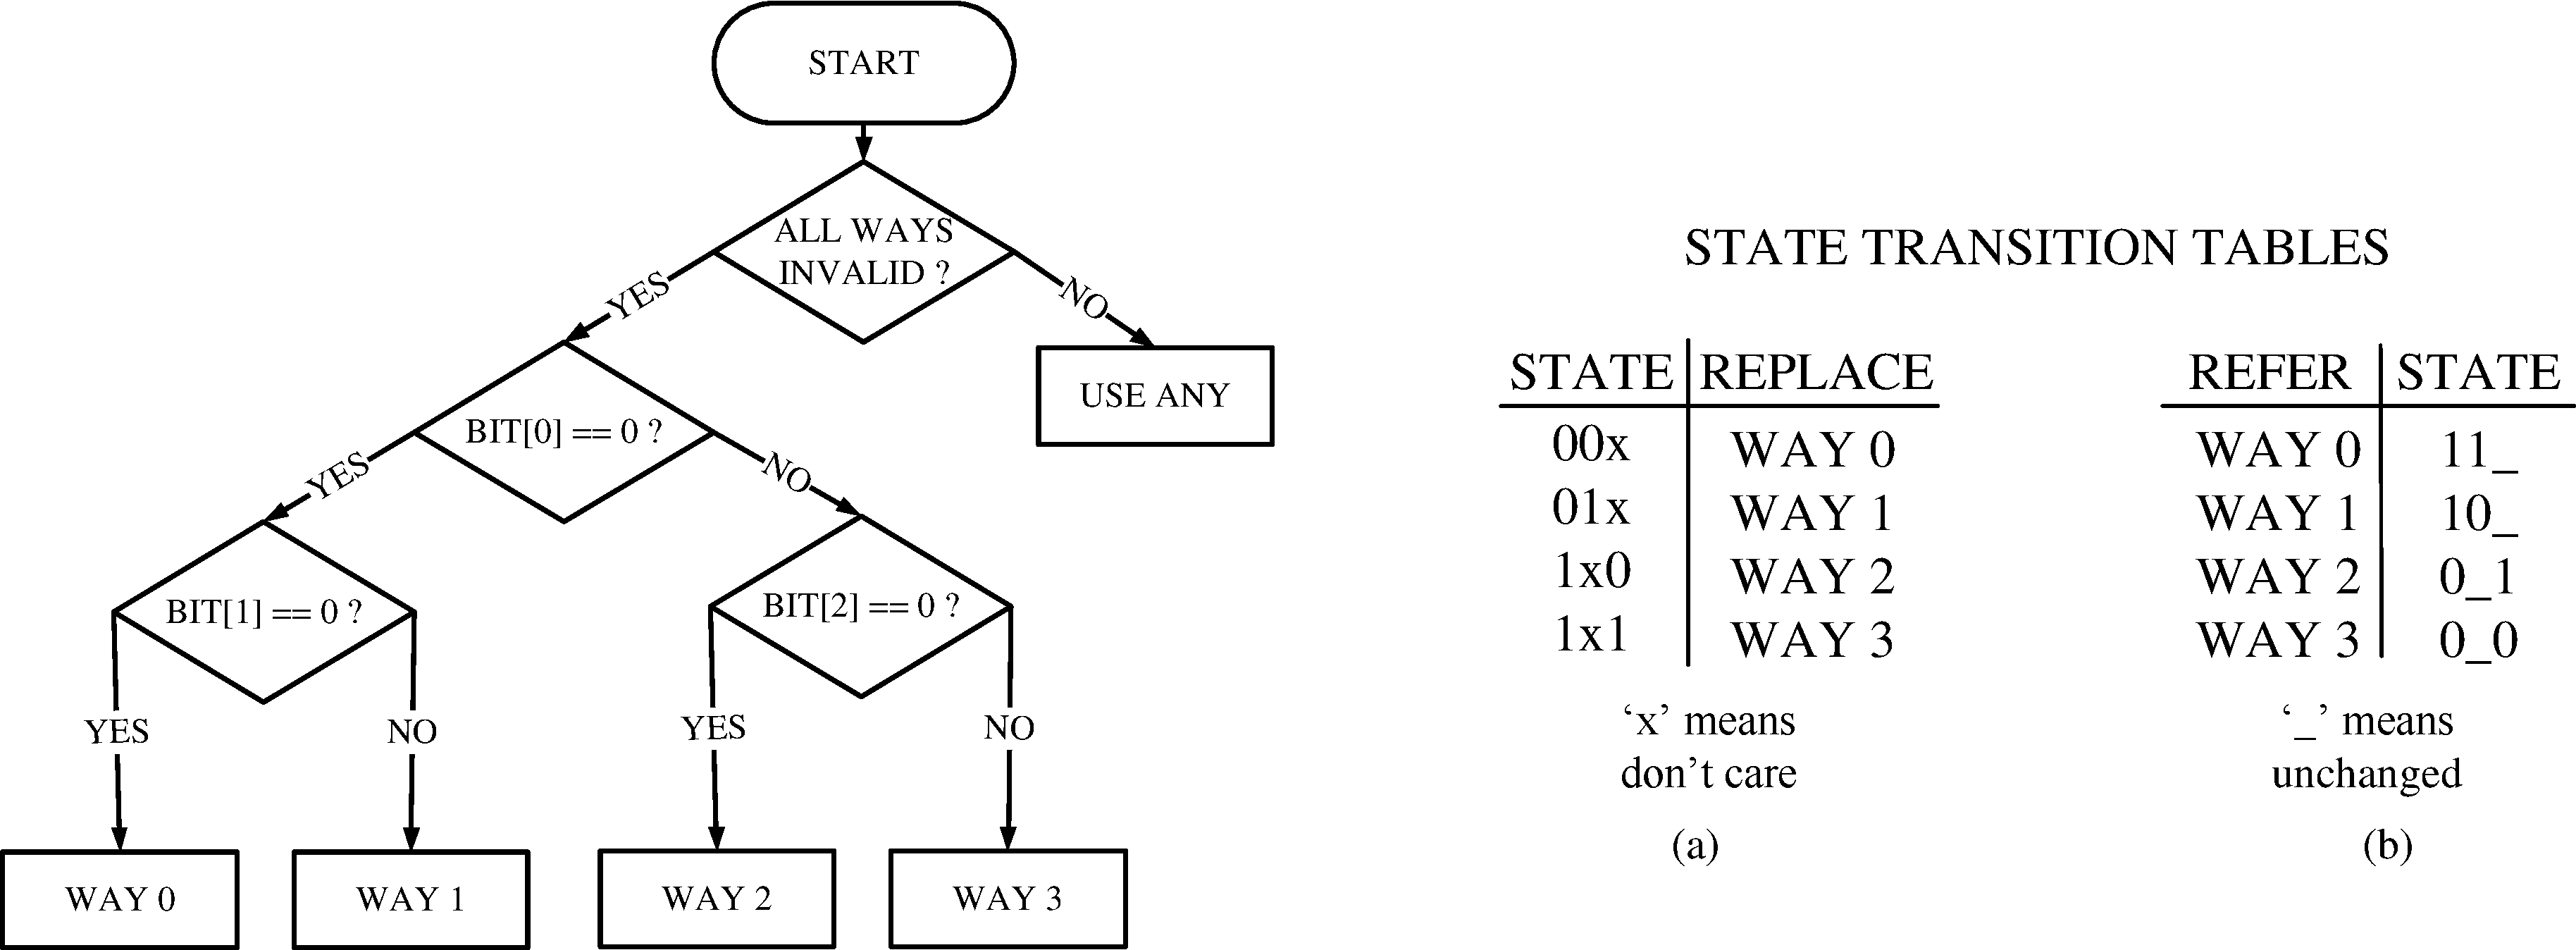
\includegraphics[width=\textwidth]{files/Figures/06-PLRU.pdf}
  \\
  \caption[Pseudo LRU]{\textbf{Pseudo-LRU decision tree and state transition table} : The flowchart on the left shows the decision making process based on the values of the 3 PLRU bits in a 4-way associative cache. The state transition tables on the right are (a) way to replace for given state (b) state to transition to on reference to a way. Reproduced from Intel Embedded Pentium Processor Family Dev. Manual\cite{manual:IntelProcessor}.}
  \label{fig:plru}
\end{figure}

\subsection{\AC\ Replacement Policy}

To reclaim the space from an \AB\, the tag bits T? (tag) and V? (valid) bits corresponding to the block are unset. The key issue is identifying the \AB\ to replace. Classical pseudo-LRU algorithms~\cite{Kedzierski-ipdps-2010,manual:OpenSparcT1} keep the metadata for the replacement algorithm separate from the tags to reduce port contention. To be compatible with pseudo-LRU and other algorithms such as DIP~\cite{qureshi-isca-2007} that work with a fixed number of ways, a set in \AC\ can be logically partitioned into $N_{ways}$. For instance, partitioning a 32 word cache set into 4 logical ways, any access to an \AB\ tag found in words 0 ---7 of the set is treated as an access to logical way 0. Finding a replacement candidate involves identifying the selected replacement way and then picking (possibly randomly) a candidate \AB{}. This procedure is repeated until the required amount of space is made available. More refined replacement algorithms that require per-tag metadata can harvest the space in the tag-word of the \AB\, which is 64 bits wide (for alignment purposes) while physical addresses rarely extend beyond 48 bits.

\section{Partial Misses} 
\label{sec:partialmiss} 

With variable granularity data blocks, a challenging although rare case (5 in every 1K accesses) that occurs is a \textit{partial miss}. It is observed primarily when the spatial locality changes.  Figure~\ref{fig:partial-miss} shows an example. Initially, the set contains two blocks from the region R, one \AB\ caches words 0 --- 2 (Region:R Start:0 End:2) and the other caches words 6 and 7 (Region:R Start:6 End:7). Let us assume that the CPU reads word 4, which misses, and the spatial pattern predictor requests an \AB\ with range Start:0 and End:7. The cache has \AB{}s that hold subparts of the incoming \AB{}, and only some words (4,5 and 5) need to be fetched.

\begin{figure}[h]
  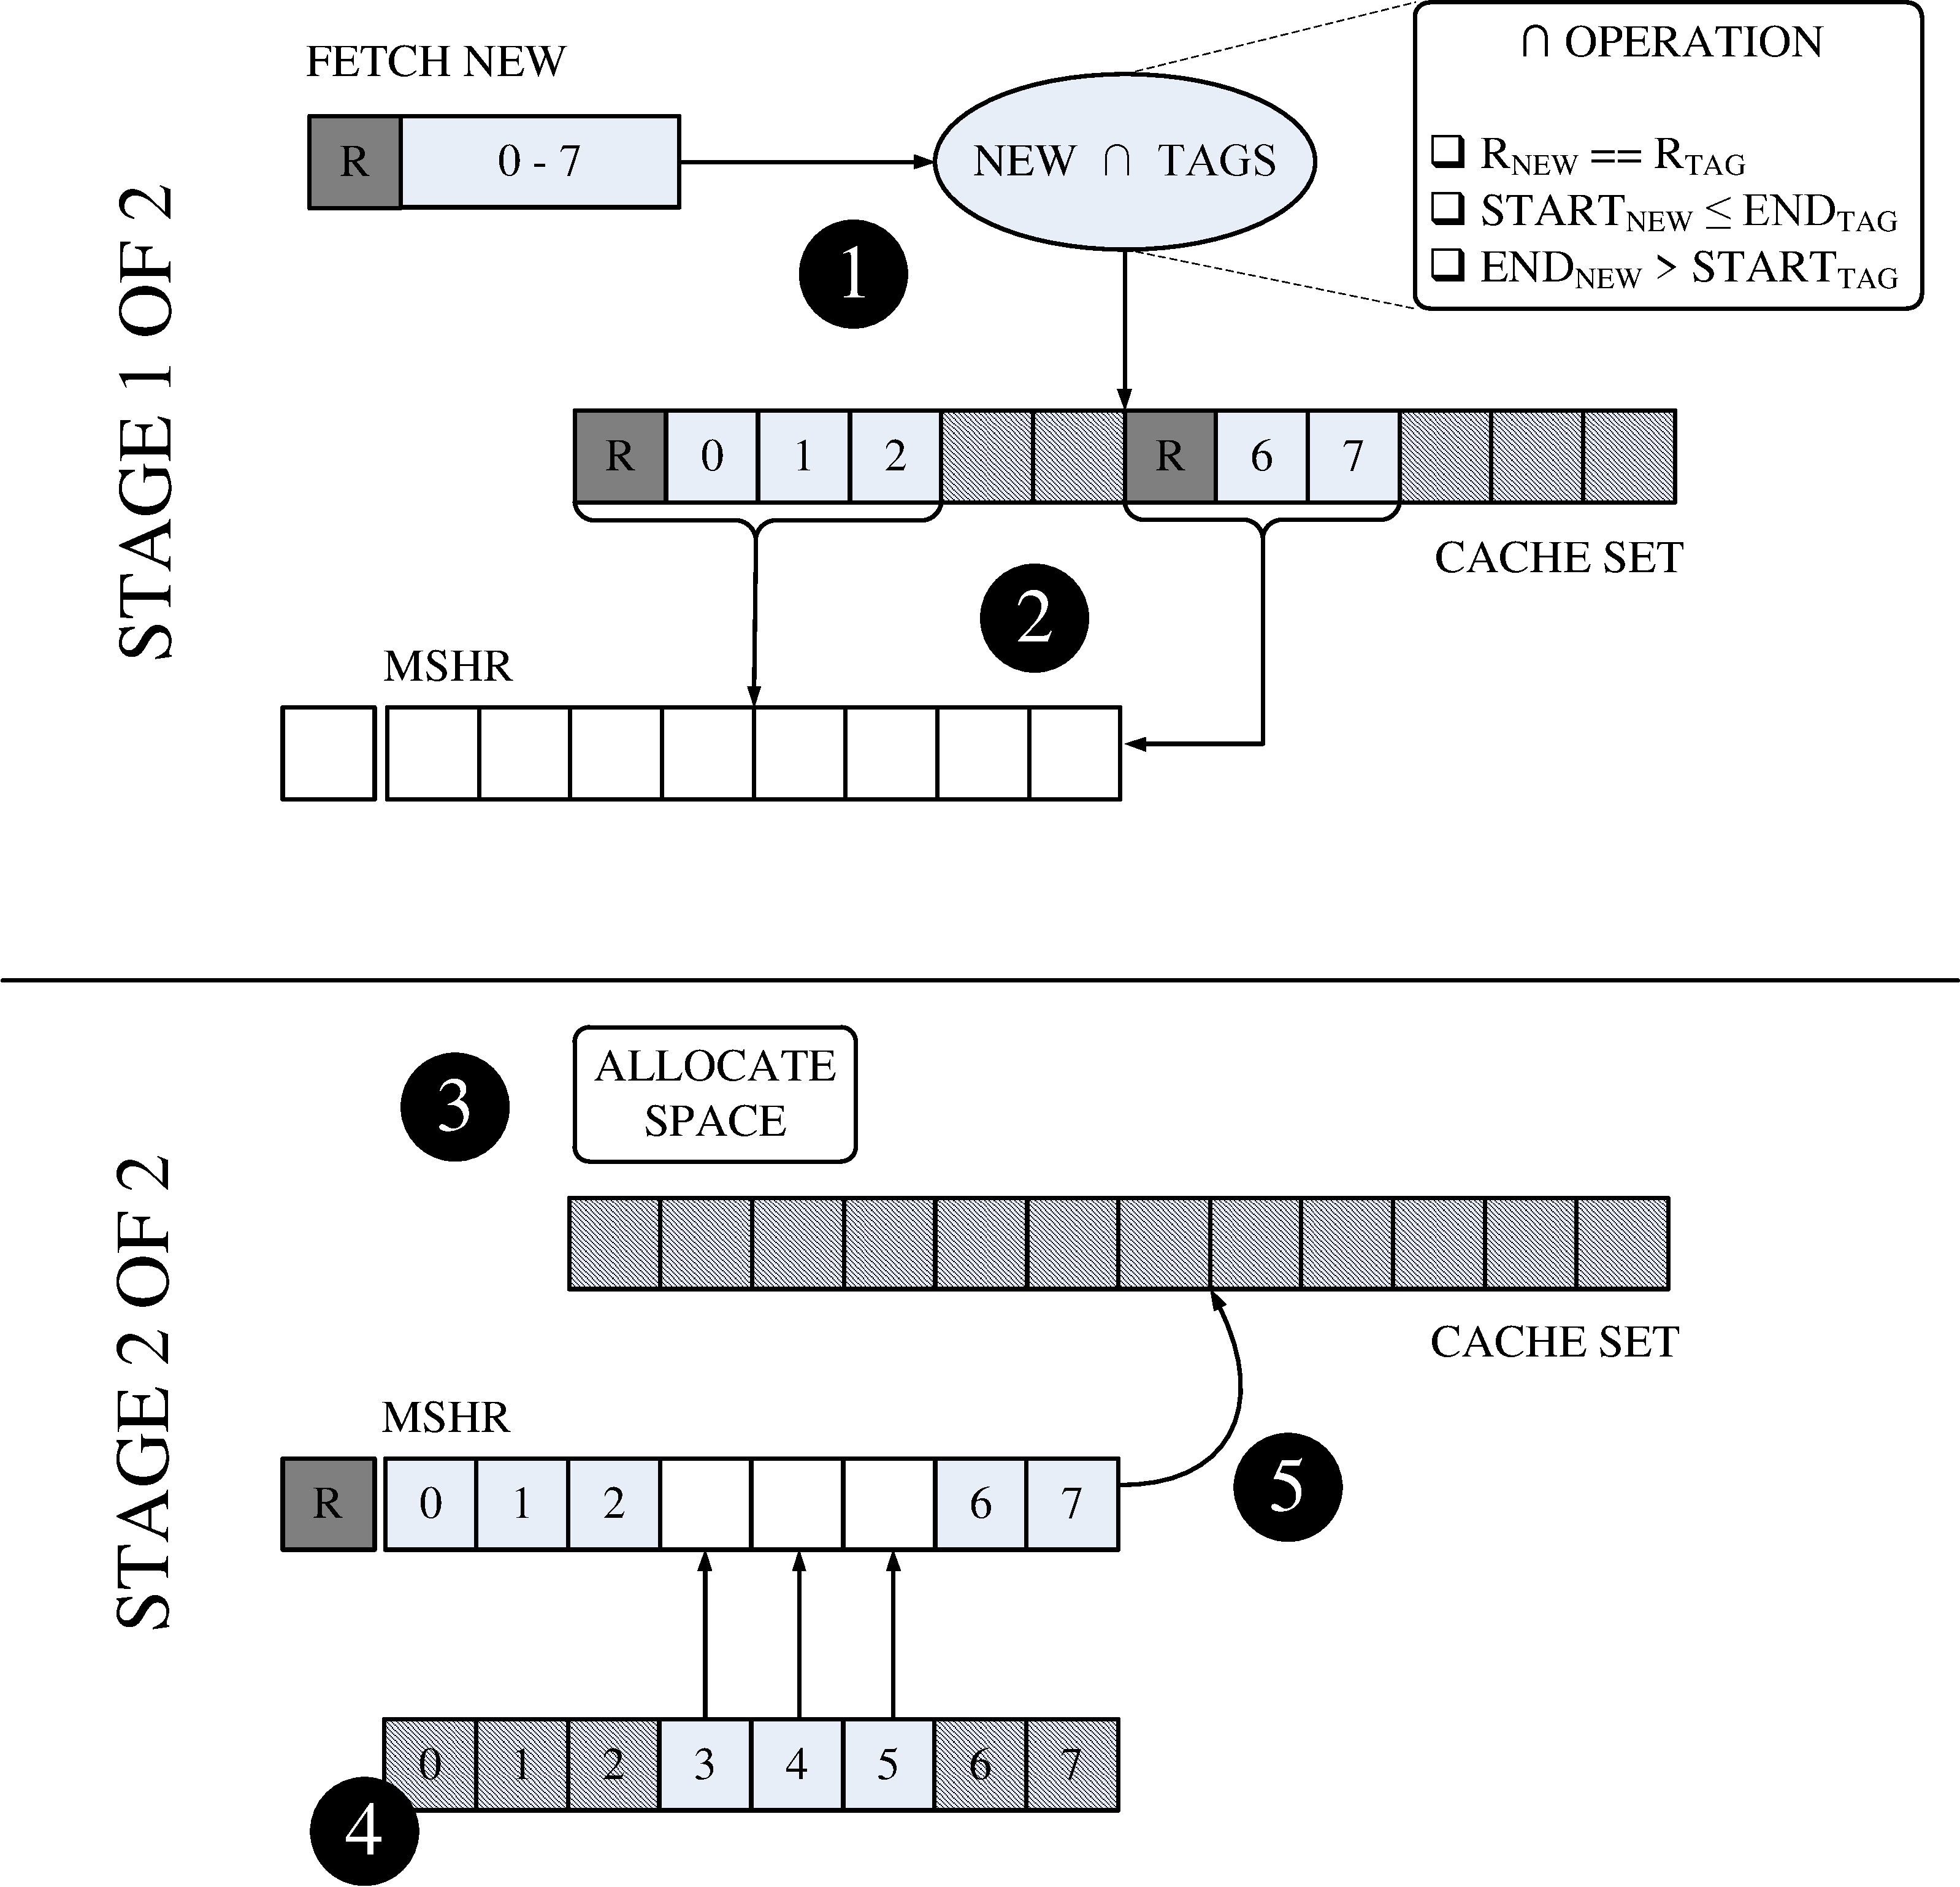
\includegraphics[width=\textwidth]{files/Figures/06-PartialMiss.pdf}
  \\
  \caption[Partial Miss]{\textbf{Partial miss processing} : The partial miss processing is shown as 2 separate stages. Stage 1 deals with the identification and eviction (to MSHR) of all overlapping blocks. Stage 2 issues the miss, allocates space for the new \AB\ and patches in the missing words from a lower level in the memory hierarchy before copying the data back into the cache set. Due to the infrequent nature of partial misses the implementation does not optimise for fetching only the missing words. }
  \label{fig:partial-miss}
\end{figure}

\clearpage

\AC\ removes the overlapping sub-blocks and allocates a new \AB{}. This is a multiple step process: \bigspot{1} On a miss, the cache identifies the overlapping sub-blocks in the cache using the tags read out during lookup. The $\cap$(in) operation returns false if there are no overlapping blocks. The $\cap$ operation consists of an equality check for the region (R), $Start_{New} \leq End_{Tag}$ and $End_{New} > Start_{Tag}$ (where \textit{New} refers to the fetch request from the spatial pattern predictor and \textit{Tag} refers to the existing \AB{}). \bigspot{2} The data blocks that overlap with the miss range are evicted and moved one-at-a-time to the miss status holding register (MSHR) entry. \bigspot{3} Space is then allocated for the new block, i.e., it is treated like a new insertion. A miss request is issued for the entire block (Start:0 --- End:7) even if only some words (e.g., 3, 4 and 5) may be needed. This ensures request processing is simple and only a single refill request is sent. \bigspot{4} The incoming data block is patched into the MSHR; only the words not obtained from the L1 (words 3,4 and 5 as indicated in Fig\ref{fig:partial-miss}) are copied (since the lower level could be stale). \bigspot{5} The entire block is copied back into the SRAM array.

\section{Spatial Pattern Predictor}
\label{sec:spatial_pattern_predictor}

The \AC\ uses a spatial block predictor, which  informs refill requests about the range of the block to fetch. \AC\ can exploit any spatial locality predictor and there have been many efforts in the compiler and architecture community~\cite{Chilimbi-Hill-pldi-1999, kumar-isca-1998, pujara-hpca-2006,chen-hpca-2004}. A tabular approach is adopted, as shown in Fig~\ref{fig:predictor}, consisting of a set of access bitmaps; each entry is \code{RMAX} (maximum granularity of an \AB{}) bits wide and represents whether the word was touched during the lifetime of the recently evicted cache block. The entry is indexed with information gleaned from either the program counter (PC) which initiated the cache miss or region tag for the effective address or both. On a miss, the predictor will search for an entry  and choose the range of words to be fetched on a miss on either side (left and right) of the critical word. The predictor optimizes for spatial prefetching and will  overfetch (bring in potentially untouched words), if they are interspersed amongst contiguous chunks of touched words. The prediction can also be bypassed when there is low confidence in the prediction accuracy, i.e. when there may not be an entry in the table. Tradeoffs in the design of the spatial predictor are evaluated in \S~\ref{sec:predictor_tradeoffs}.


\begin{figure}[h]
  \centering
  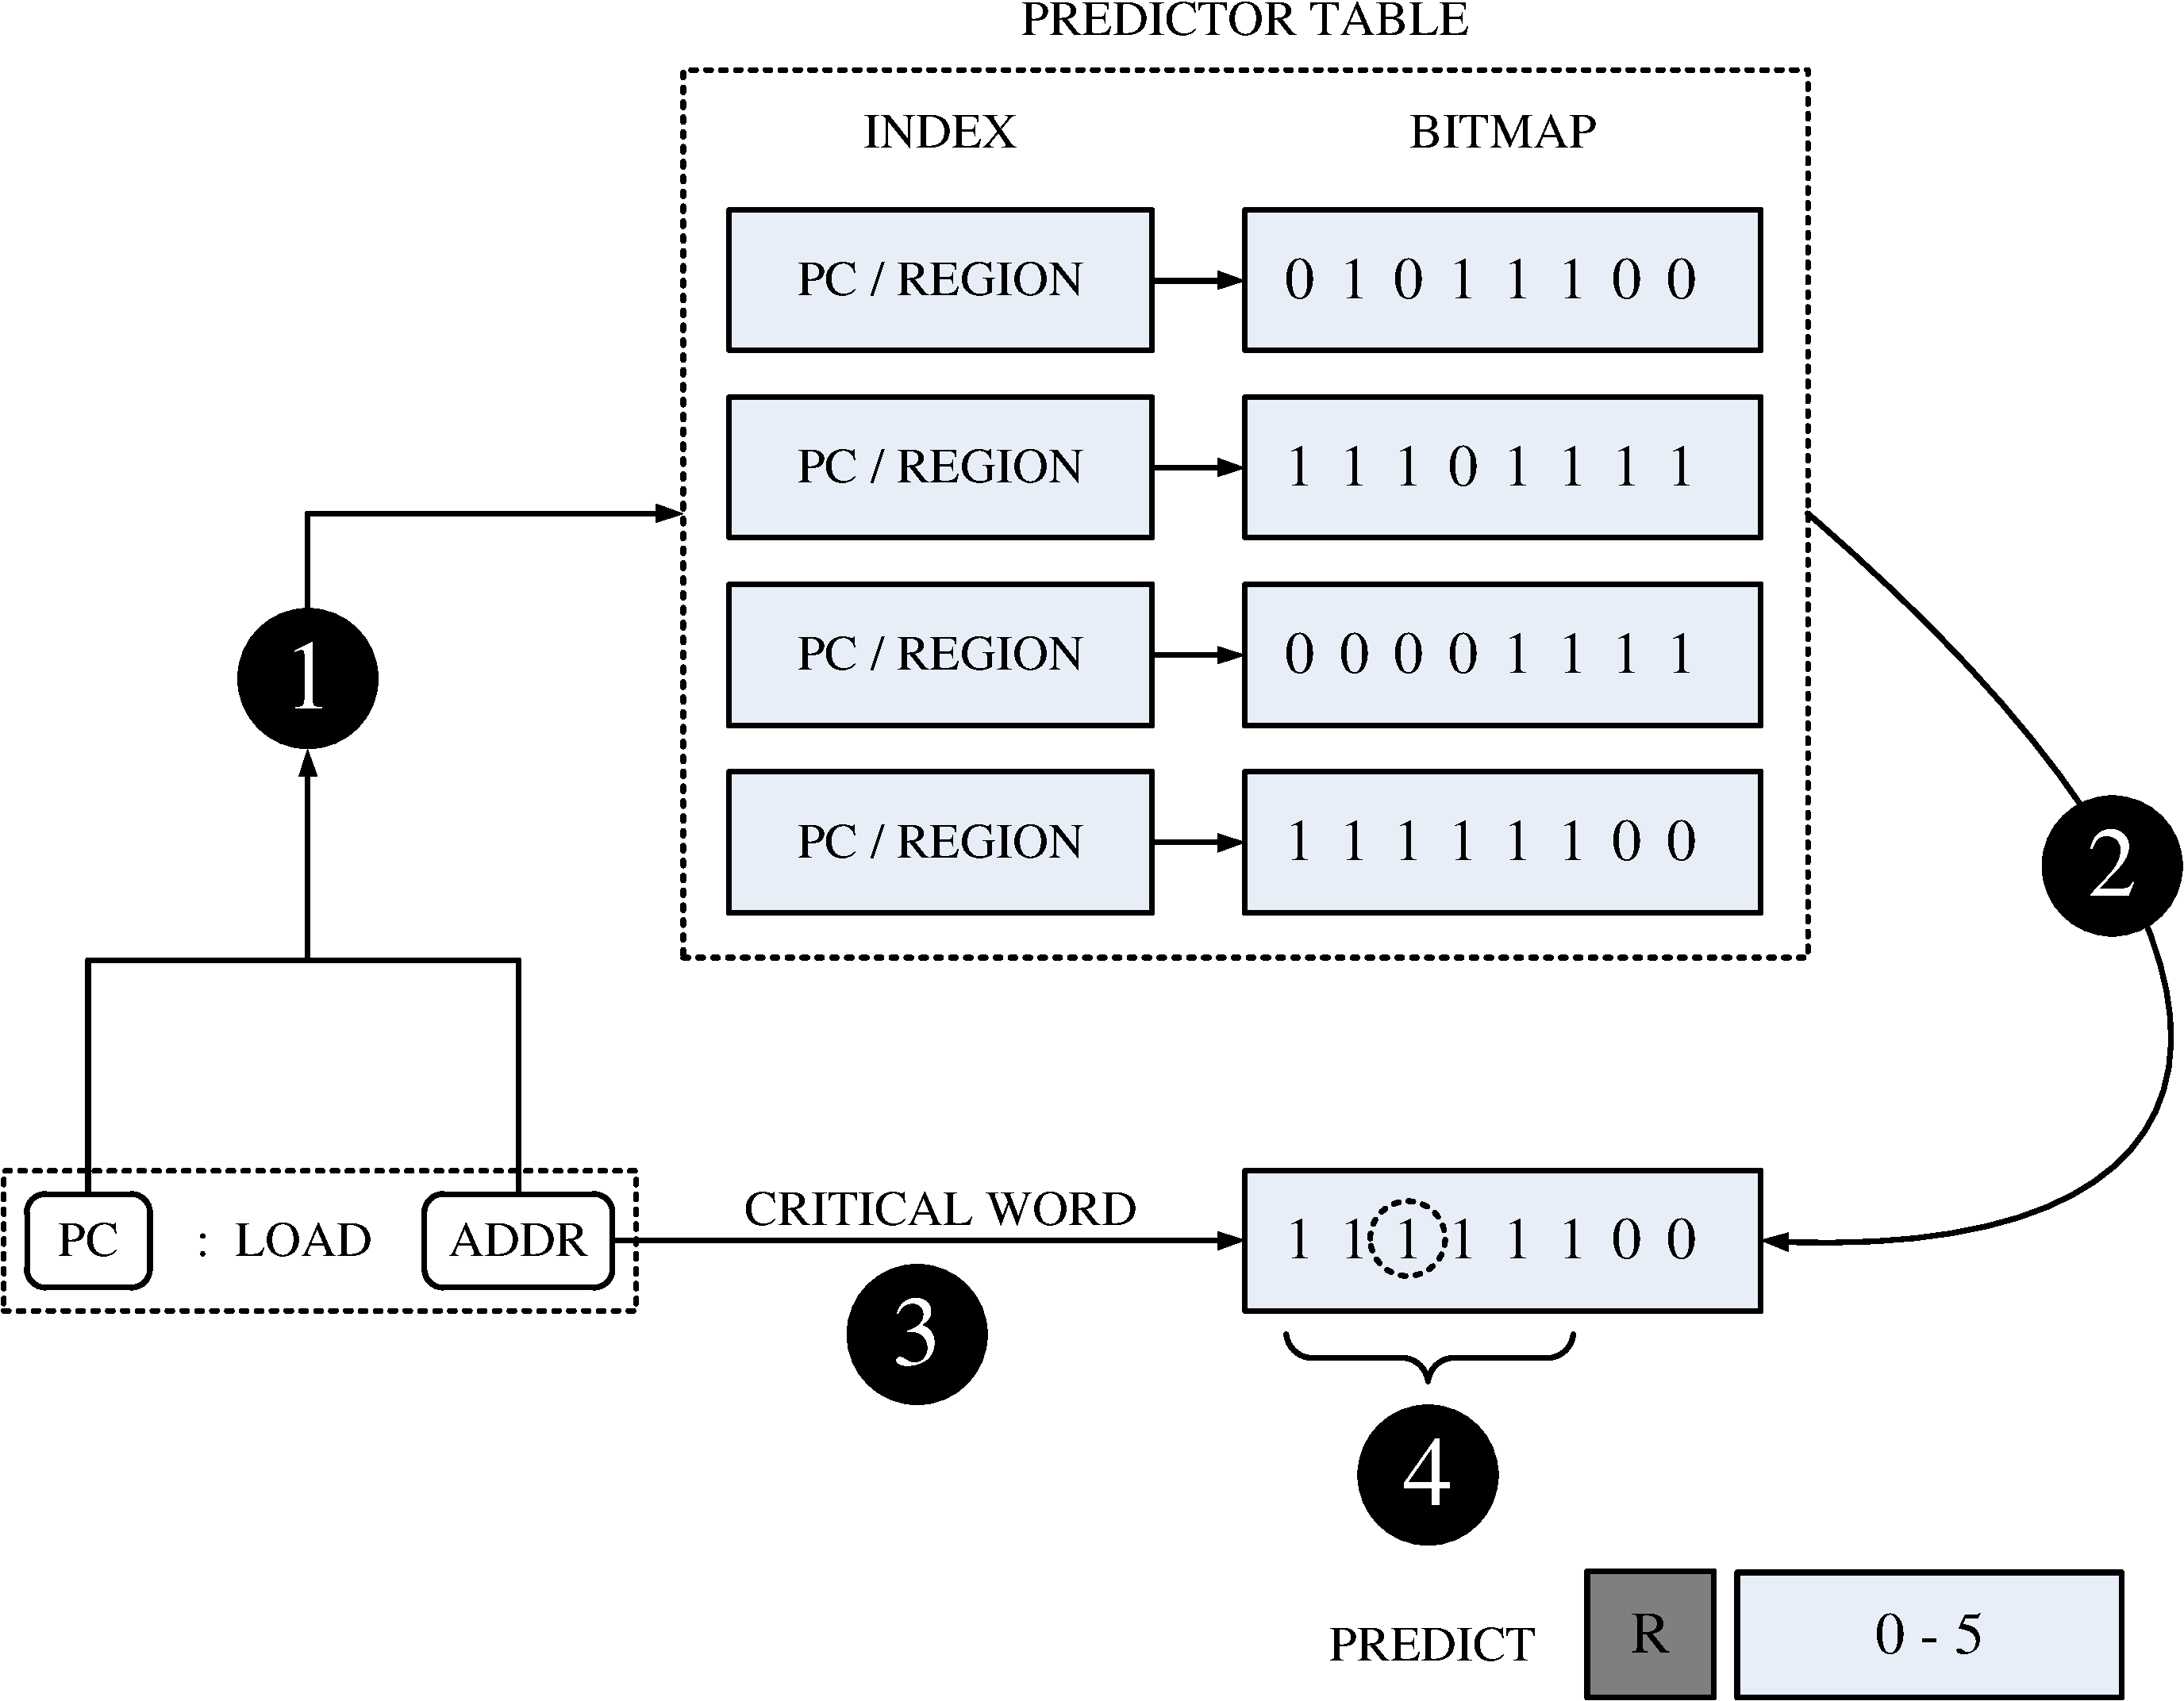
\includegraphics[width=0.75\textwidth]{files/Figures/06-Predictor.pdf}
  \\
  \caption[Amoeba-Cache Predictor]{\textbf{\AC\ Predictor} : On a cache miss, the \AC\ predictor performs the following steps. \bigspot{1} Lookup the table using bits from the program counter or region tag or a combination of both. \bigspot{2} If an entry is present for the calculated index, the corresponding bitmap is read out from the table. The bitmap is updated on eviction of a cache block with the pattern of words accessed by the CPU in the cache block during its lifetime. \bigspot{3} The critical word (word requested by the instruction) is examined to ensure it is part of the marked portion of the bitmap. The range(\code{START} and \code{END}) for the new block is extended to include all marked words in the bitmap. \bigspot{4} The predictor then requests the cache to issue a miss for words 0 -- 5 based on the bitmap pattern.}
  \label{fig:predictor}
\end{figure}

\section{Related Work}

This section describes prior work in the area which closely relate to the \AC{}. 

\subsection{Line Distillation}

\begin{figure}[h]
  \centering
  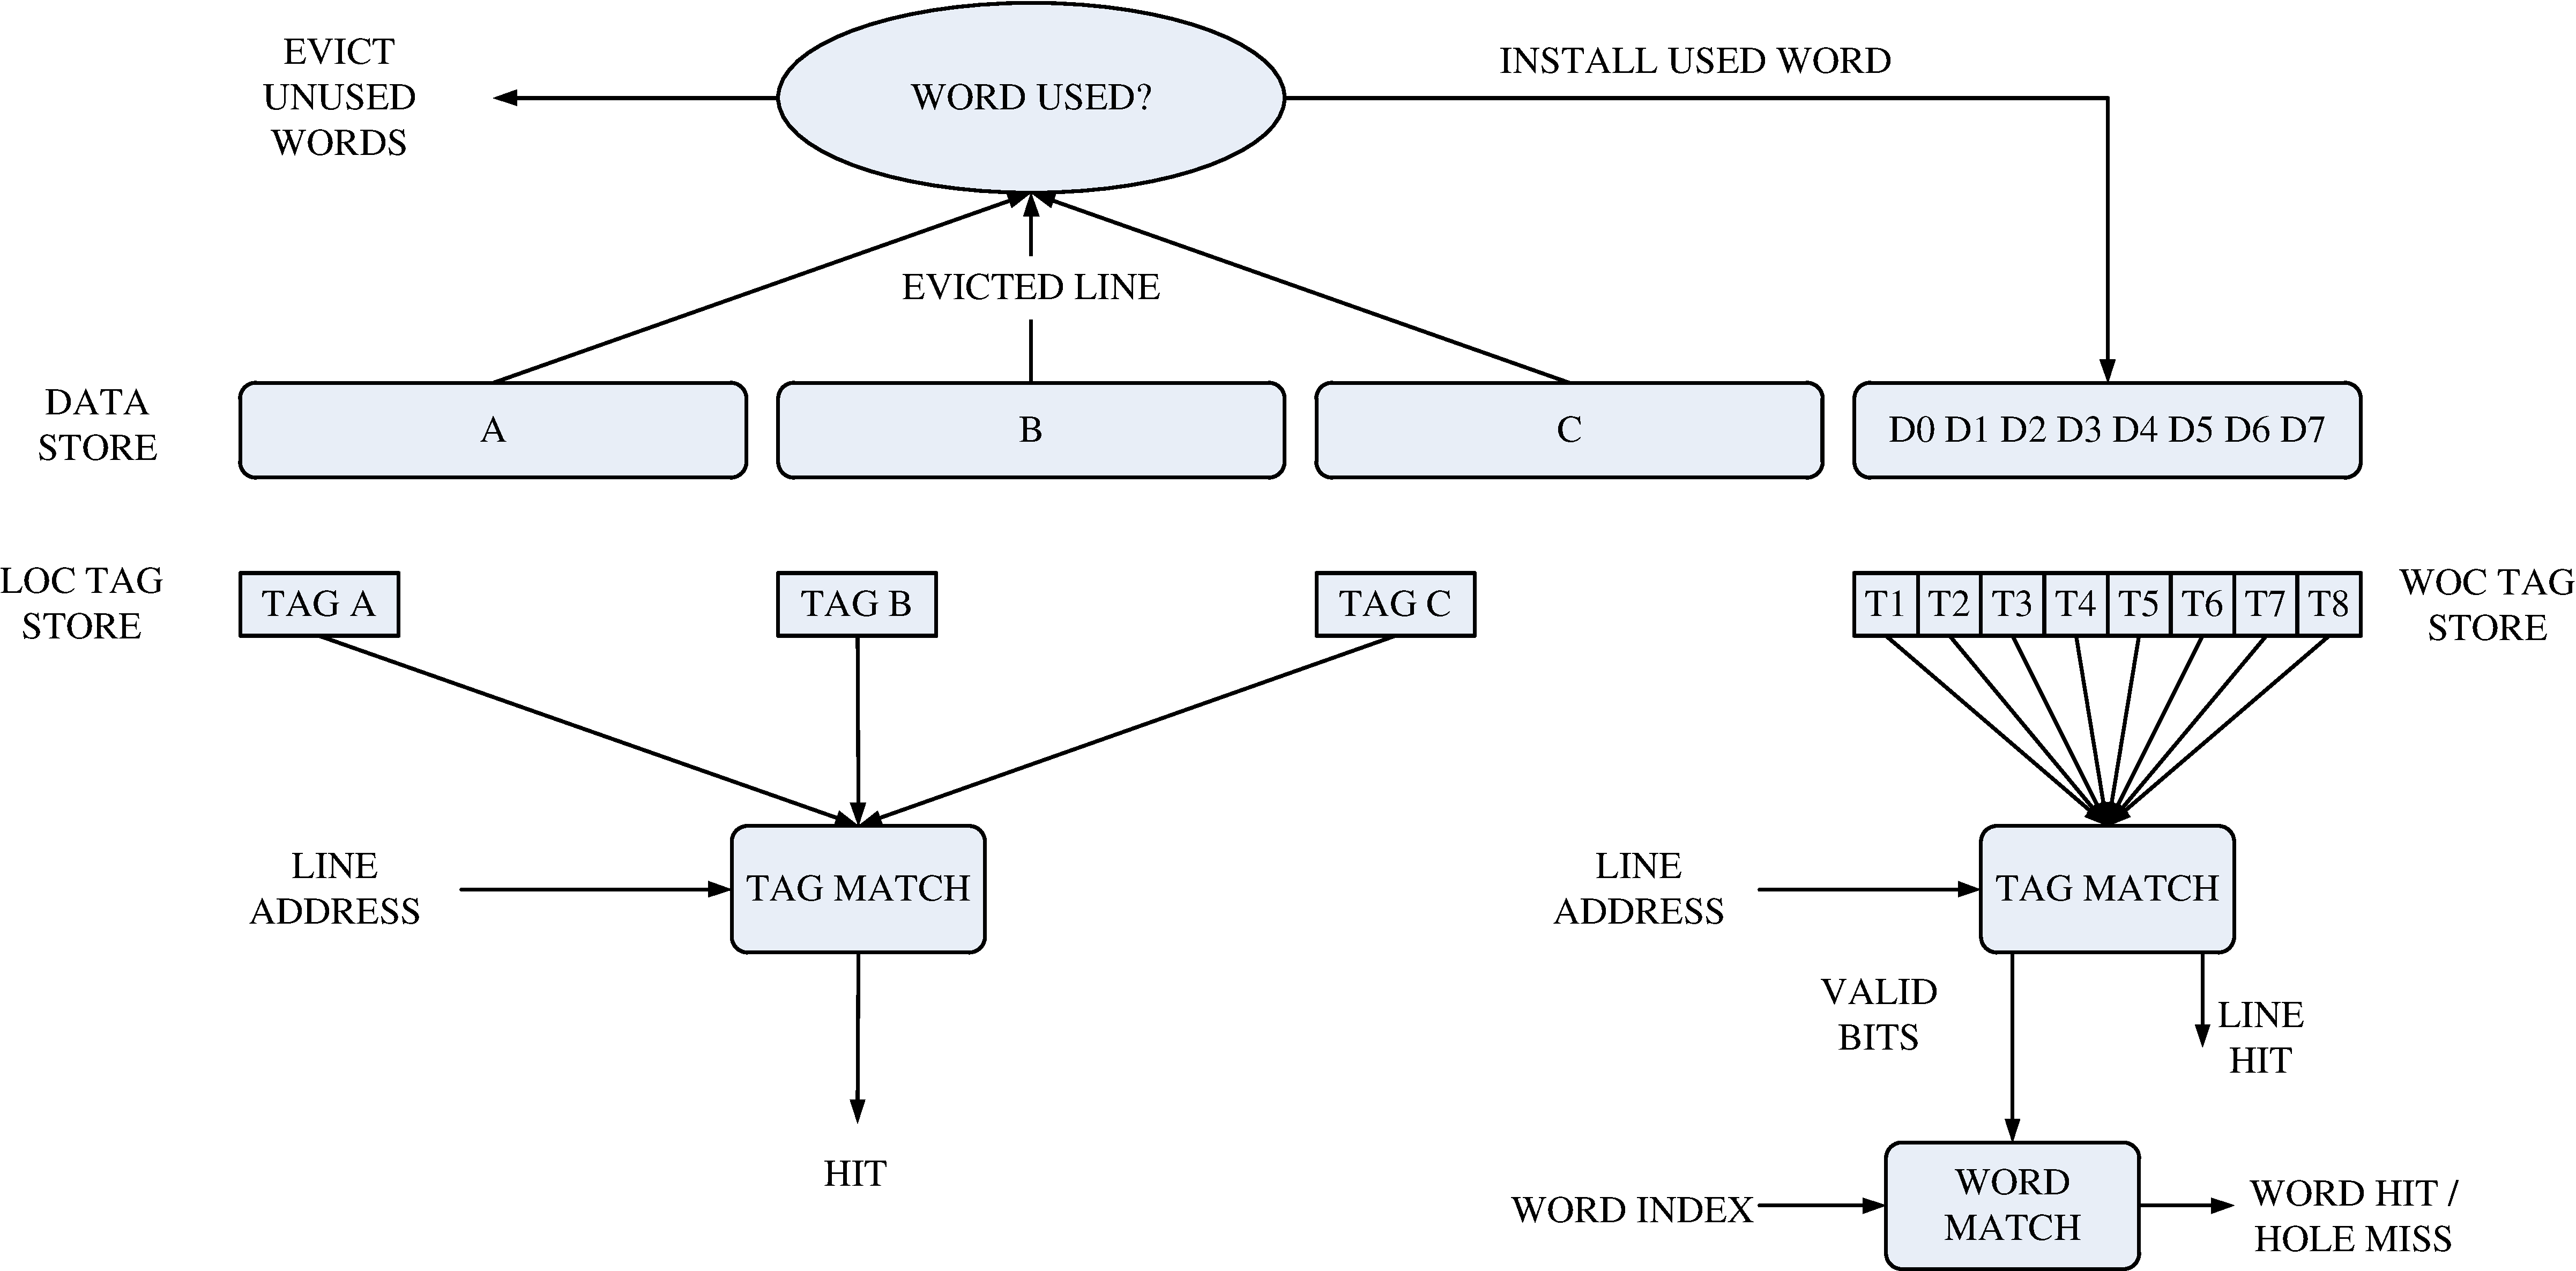
\includegraphics[width=\textwidth]{files/Figures/06-LDIS.pdf}
  \\
  \caption[Line Distillation]{\textbf{Line Distillation Organisation} : The figure shows a single set from a 4-way \textit{Distill Cache}. The LOC consists of ways A,B and C and the WOC consists of way D. A line evicted from the LOC ways is checked for suitable words to retain in the WOC. A lookup in the WOC includes a check for the line address as well as the word index to qualify as a hit.}
  \label{fig:ldis}
\end{figure}

Qureshi et al\cite{Qureshi:2007:LDIS} proposed a cache organisation dubbed as the \textit{Distill Cache} and a technique known as \textit{Line Distillation} to discard only the unused words from a cache line upon eviction. Their proposed organisation (as shown in Fig~\ref{fig:ldis}) includes a \textit{Line Organised Cache(LOC)} which stores blocks at the default line granularity (such as 64 bytes per line) and a \textit{Word Organised Cache(WOC)} which stores blocks at the granularity of a word (usually 8 bytes). The WOC is similar in spirit to the \textit{Victim Cache}\cite{Jouppi:1990:IDC:325164.325162} proposed by Jouppi. The victim cache is a small, fully associative cache which is usually coupled with a direct mapped cache and stores the victim of a cache miss. It was used to alleviate problems caused by conflict misses. The WOC however, does not cache the entire block. The WOC only caches the words within the cache block which were touched by the application at the time of eviction. Whether the words will be installed in the WOC or the entire line is discarded is determined by the number of words which were touched. The authors propose a \textit{median threshold filtering} policy, where the words are retained in the WOC on eviction only if the number of words touched in the cache line from the LOC is less than the median number of words touched in a cache block in the application. The authors propose the implementation of the \textit{Distill Cache} at the L2 as the design of the L1 data cache is is heavily constrained by cycle time and out of order processors already cover some of the latency of the cache misses. Their findings show an average improvement of 12\% in IPC by reducing cache misses for a 1MB 8-way L2 by 30\%.

The \textit{Distill Cache} is similar to the \AC\ in the sense that in a single cache it supports word granularity blocks and line granularity blocks as two extremes. The \AC\ supports varying granularity blocks of sizes 1--\textit{RMAX} words (see \S~\ref{sec:amoeba_blocks_and_set_indexing}). The WOC always incurs a high overhead in terms of a single tag for each of the data words in the WOC which is similar to the worst case scenario for an \AC\ where all the data words in the cache set are of size 1 word. Veidenbaum et al\cite{Veidenbaum:1999:ACL:305138.305188}, propose the entire cache be word organised and propose an online algorithm to prefetch required words. This approach however has a built in tag overhead of 50\% and requires energy intensive associative searches.

\subsection{Sector Caches}

The original cache designs\cite{liptay68} were essentially sector caches in nature was due to the technology available at the time (the discrete transistor logic for sectors was easier to implement) where the cache consisted of sectors (address tags) and subsectors (or blocks with valid bits). They were deprecated in favor of set associative caches which have superior performance in terms of miss rate and because many subsectors went unused due to early eviction of a sector (for a 64K data cache with 256 byte sector frame and 64 byte sector size had only 74\% utilization\cite{Rothman_Smith_2000}).
\\
\begin{figure}[h]
  \centering
  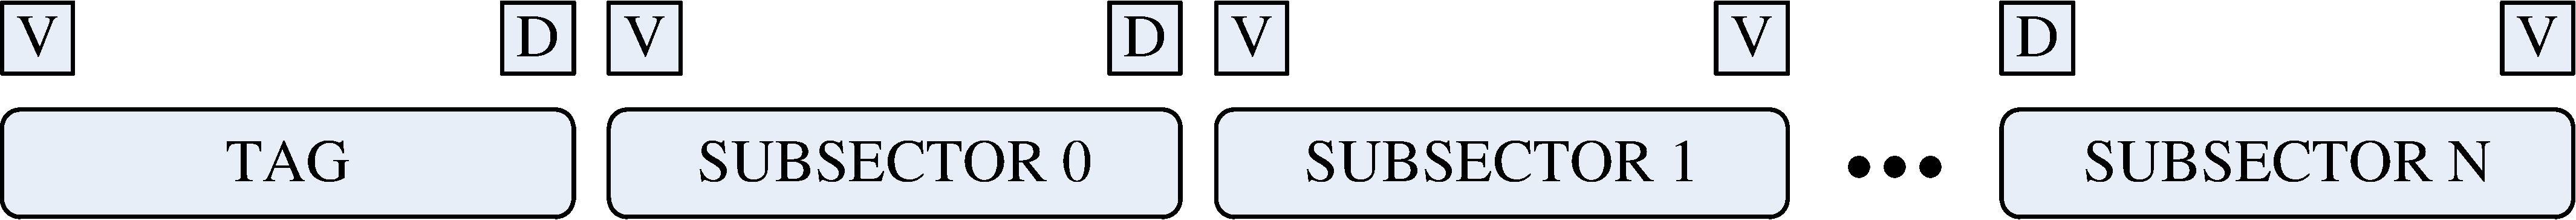
\includegraphics[width=\textwidth]{files/Figures/06-Sector.pdf}
  \\
  \caption[Sector Frame]{\textbf{Sector Frame} : Diagram of a single sector frame (reproduced from \cite{Rothman_Smith_2000}). \textit{D} is the dirty bit  and \textit{V} is the valid bit associated with the subsector. The first documented use of a cache in a computing system, the IBM 360/85, was 16 KBytes in size and consisted of 16 sector frames of 16 subsectors, each of size 64 byte blocks.}
  \label{fig:sector_frame}
\end{figure}

In the 90's interest in sector cache design was revived by Rothman et al\cite{Rothman_Smith_2000} and Seznec\cite{Seznec-decoupled-sector-cache-isca, seznec:inria-00074588} due to their suitability for large cache design. Sector caches are also desirable due to reduced bus traffic and smaller latency overheads.  The Intel Pentium 4, SUN SPARC and IBM PowerPC G4/G5 all incorporated sector designs into the cache memory hierarchy. The Power7 architecture also employs a sector design at the L2 with 32 bytes per subsector. Sector caches can also be combined with victim caches as proposed by Lai et al\cite{Lai-victim-sector} to reduce miss rates. Prior work on spatial pattern predictors by Kumar et al\cite{kumar-isca-1998}, Pujara et al\cite{pujara-hpca-2006} and Yoon et al\cite{Yoon_Jeong_Erez_2011, yoon2012dgms} use sector caches as the substrate for their proposals.

Sector caches provide variable granularity caching at the granularity of the subsector size. However, the space freed up by unused subsector cannot be reused by a different sector frame. The \AC\ is able to provide adaptive granularity caching at a granularity of a word and the unused space can be used by \AB{}s from other regions. Decoupled sector caches\cite{Seznec-decoupled-sector-cache-isca} help reduce the number of invalid subsectors within a sector by increasing the number of tags per sector. Compared to the \AC{}, the tag space is a constant overhead and limits the number of invalid sectors that can be eliminated. Pujara et al\cite{pujara-hpca-2006} consider a word granularity sector cache and use a predictor to try and bring in only the used words. Our observations show (see Fig~\ref{fig:ac_comparison}) that smaller granularity sectors increase misses and optimisations that prefetch can pollute the cache and interconnect with unused words.

\subsection{Indirect Index Caches}
\label{sec:indirect_index_caches}
\textit{Indirect index caches}(IIC) were proposed by Hallnor et al.\cite{Hallnor_Reinhardt_2000} as a practical, fully associative, software managed secondary cache system that does not require OS or application intervention. Their goal was to provide LLCs the benefits of full associativity and software management similar to DRAM architectures. Their motivation was the magnitude of the increasing gap in latency between LLC and DRAM which is similar to the existing gap between DRAM and disk. In a conventional cache each way is statically associated with a tag entry and indicates whether the way is valid. In the IIC, the tag entries are not associated with particular data entries (ways). A tag entry in the IIC contains a pointer to the data block, i.e. an index into the cache's data array. And since a tag entry can indicate any data array location, the cache is fully associative. Figure~\ref{fig:iic} illustrates an example IIC design. 

The tag storage requirement for the IIC is greater than a conventional cache as the position of an entry in the tag store for the IIC is not related to the corresponding physical address of the block. Assuming a 48-bit physical address for a 1M cache with 256 byte blocks, the tag entry in the primary tag storage, as shown in Figure~\ref{fig:iic}, consists of tag bits ($48-\log_{2}(256) = 40$ bits), status bits (3 bits - valid, dirty and unreferenced), the index of the data block in the data array ($\log_{2}(1M/256) = 12$ bits), chain pointer ($\log_{2}(1M/256) = 12$ bits) and replacement policy data storage (32 bits). Thus each tag entry is 99 bits in size. The latency overheads for the IIC are caused by : serial access of tag and data, additional hit and miss latency overhead due to hash table lookups and additional miss latency due to software management. 

\begin{figure}[h]
  \centering
  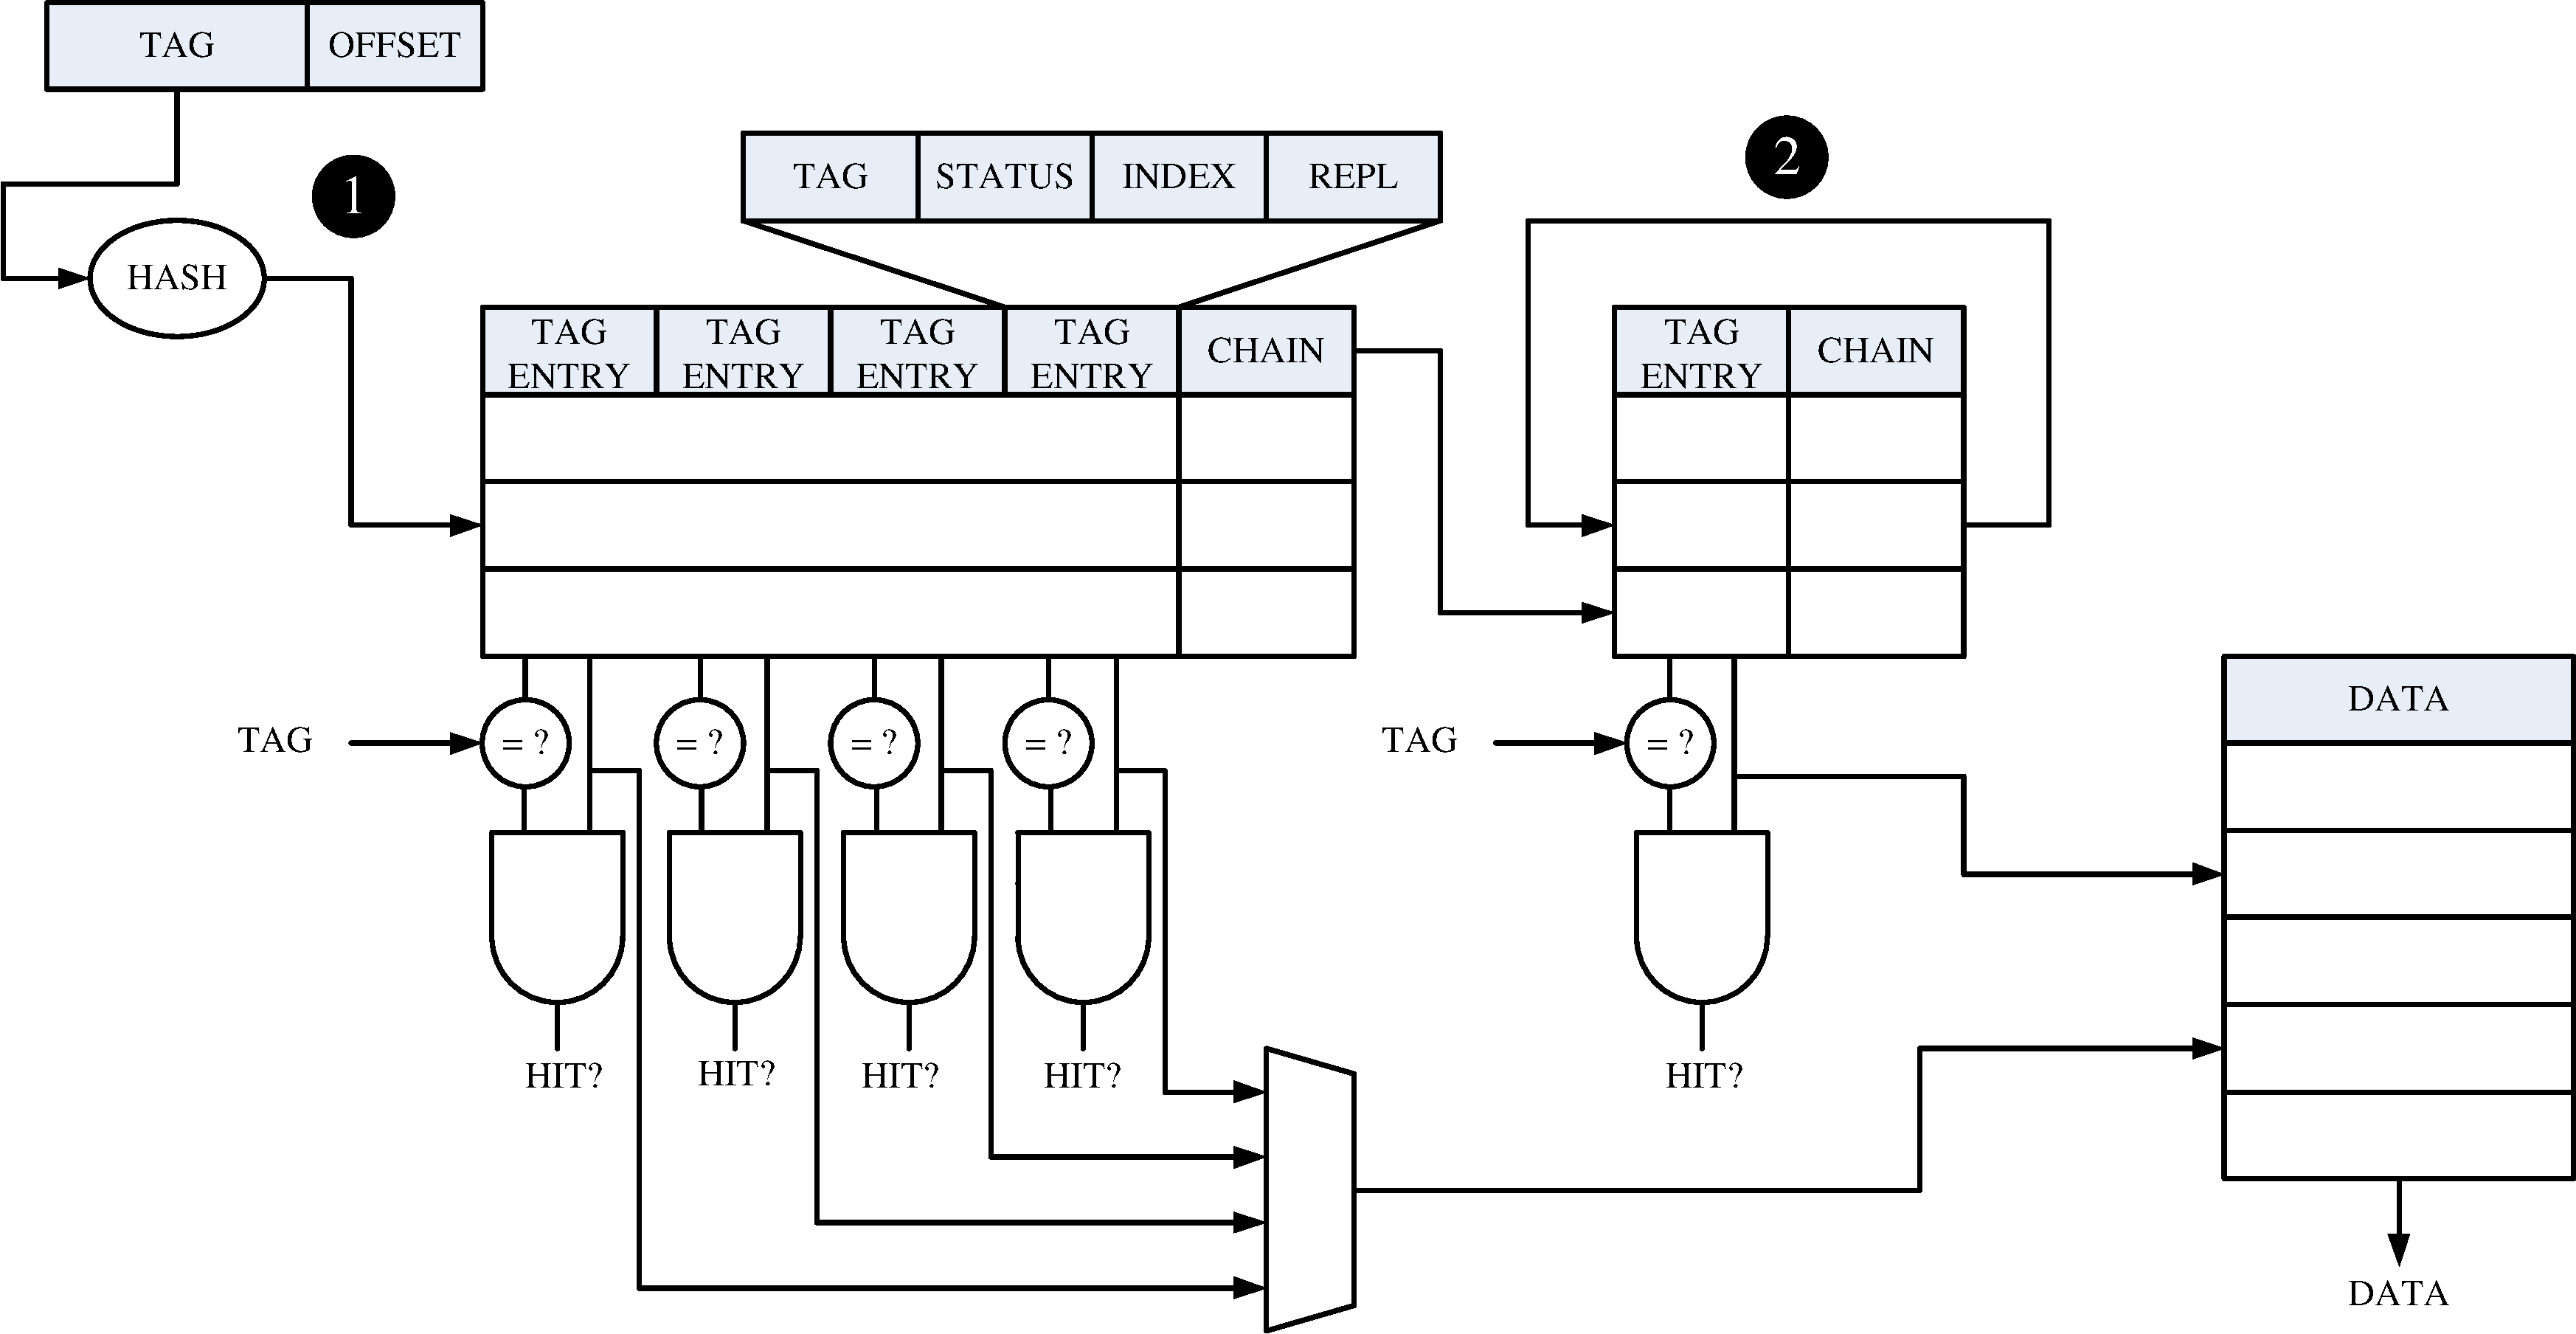
\includegraphics[width=\textwidth]{files/Figures/06-IIC.pdf}
  \\
  \caption[Indirect Index Cache]{\textbf{Indirect Index Cache} : The tag array for an IIC is split into two parts. A primary hash table and a secondary block for chaining. \bigspot{1} On each access, the block tag is hashed to obtain a primary table index. The primary table is associative, so a single search accesses the first few entries (4 in the example figure) of the hash chain. Collisions beyond this depth are chained into the secondary hash storage as shown in \bigspot{2}.}
  \label{fig:iic}
\end{figure}

In 2004, Hallnor et al\cite{Hallnor04acompressed} proposed a compressed memory hierarchy based on the IIC. Their design to support compression in the LLC was heavily inspired by IBM's Memory Expansion Technology(MXT)\cite{Pinnacle:2001}. The IIC already supported the random placement of blocks within a set with the index of the data block being stored in tag entry. With suitable modifications, the IIC was made to support compressed, variable granularity blocks. 

The IIC-Compressed design is similar to the \AC\ in the sense that it can cache variable granularity data blocks. However, the increased tag structure complexity and nature of serialised access to tags and data detract from its merits. The goals of caching variable granularity data blocks are different for the \AC{}(bandwidth and energy reduction) and the IIC(caching compressed blocks). 

\subsection{Other related work}

Recently Yoon et al. have proposed an adaptive granularity DRAM architecture\cite{Yoon_Jeong_Erez_2011}. This provides the support necessary for supporting variable granularity off-chip requests from an Amoeba-Cache-based LLC. Some research \cite{Dubnicki:1992:ABS:139669.139725,Choi:2011:DRM:2120965.2121416} has also focused on reducing false sharing in coherent caches by splitting/merging cache blocks to avoid invalidations. They would benefit from the Amoeba-Cache design, which manages block granularity in hardware. There has a been a significant amount of work at the compiler and software runtime level (e.g. \cite{Chilimbi-Hill-pldi-1999}) to restructure data for improved spatial efficiency. There have also been efforts from the architecture community to predict spatial locality \cite{pujara-hpca-2006, Watkins:2008:RCB:1505816.1505849, kumar-isca-1998, yoon2012dgms}, which can be used to predict Amoeba-Block ranges. Finally, cache compression is an orthogonal body of work that does not eliminate unused words but seeks to minimize the overall memory footprint \cite{AlameldeenPHD}.


%!TEX root=/home/ska124/Dropbox/Thesis/thes-full.tex

%%%%%%%%%%%%%%%%%%%%%%%%%%%%%%%%%%%%%%%%%%%%%%%%%
%
%     Chapter 4   
%
%%%%%%%%%%%%%%%%%%%%%%%%%%%%%%%%%%%%%%%%%%%%%%%%

\chapter{Implementation}
\label{chap:hardware_complexity_and_simulation}

This chapter describes the additional hardware complexity added to an \AC\ with respect to a conventional cache in order to support variable granularity \AB{}s. The chapter also describes the simulation infrastructure used to evaluate the performance of the \AC{}.

\section{Hardware Complexity}  
\label{sec:hardware_complexity}

The complexity of the \AC\ is analysed along the following directions:
\begin{itemize}
  \item Additional complexity of the cache controller
  \item Area, latency and energy overhead
  \item Challenges of megabyte sized \AC{}s
\end{itemize}


\subsection{Cache Controller} 

Each level of the cache memory hierarchy incorporates a finite state machine (FSM) called the \textit{cache controller} to track the state of the blocks currently being cached. The cache controller is the interface between the CPU, cache and DRAM as shown in Fig~\ref{fig:cache_controller_basics}(a). The figure depicts a look through hierarchy where the processor is isolated from the system, thus allowing the processor to run with data from the cache while another bus master is acessing main memory. Fig~\ref{fig:cache_controller_basics}(b) shows an overview of the implementation logic for the cache controller. Using the current state of the block and the incoming request ( which could be from the CPU, DRAM or a remote cache) a new state is set for the cache block. The state transition diagram of an L1 \AC\ is shown in Fig~\ref{fig:L1protocol}. The FSM for the \AC\ is a superset of an equivalent FSM for a conventional cache (without cache coherence; more details in \S~\ref{sec:coherence}).

\begin{figure}[h]
  \subfloat[Interface]{
    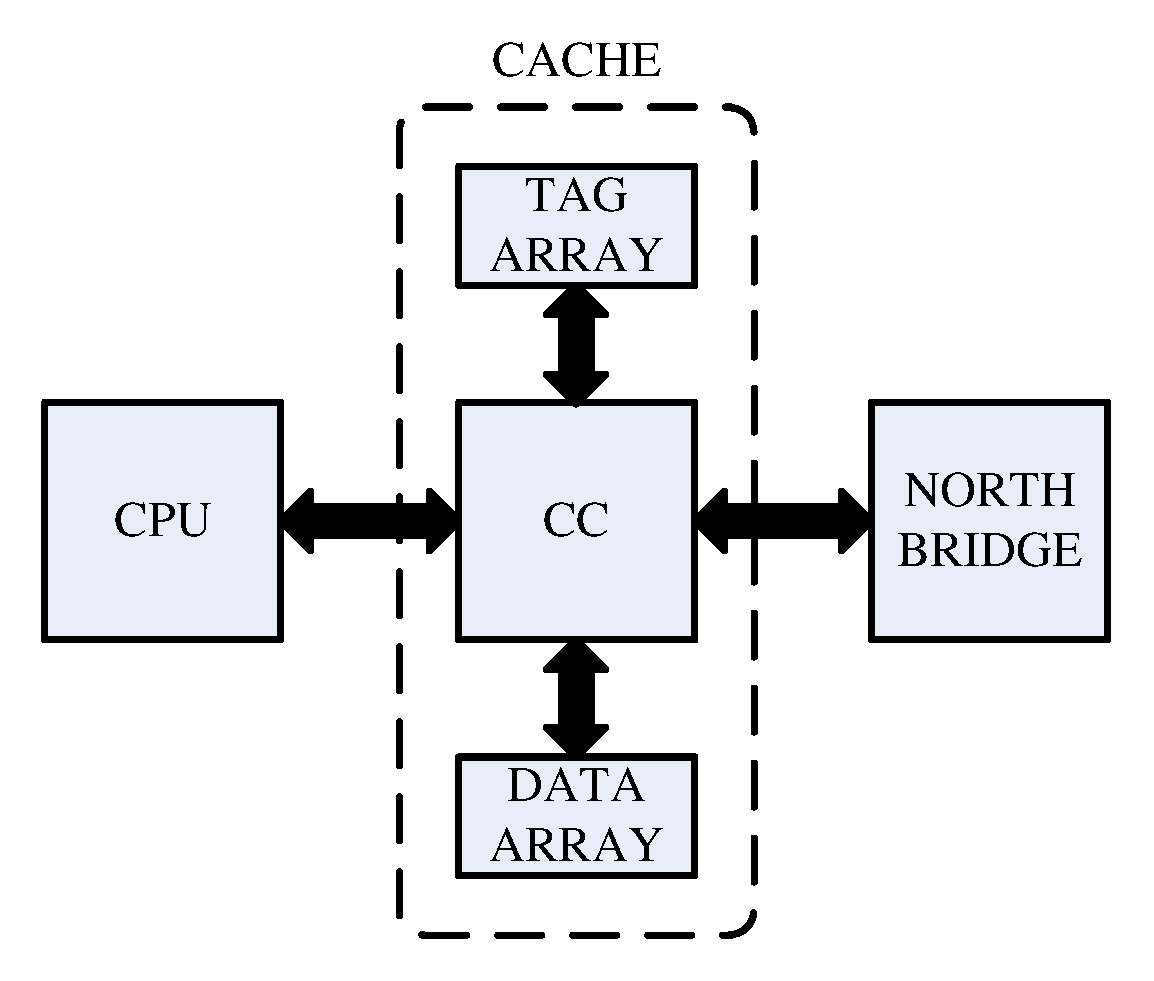
\includegraphics[width=0.5\textwidth]{files/Figures/07-LookThroughArchitecture.pdf}
  }
  \subfloat[FSM Logic]{
     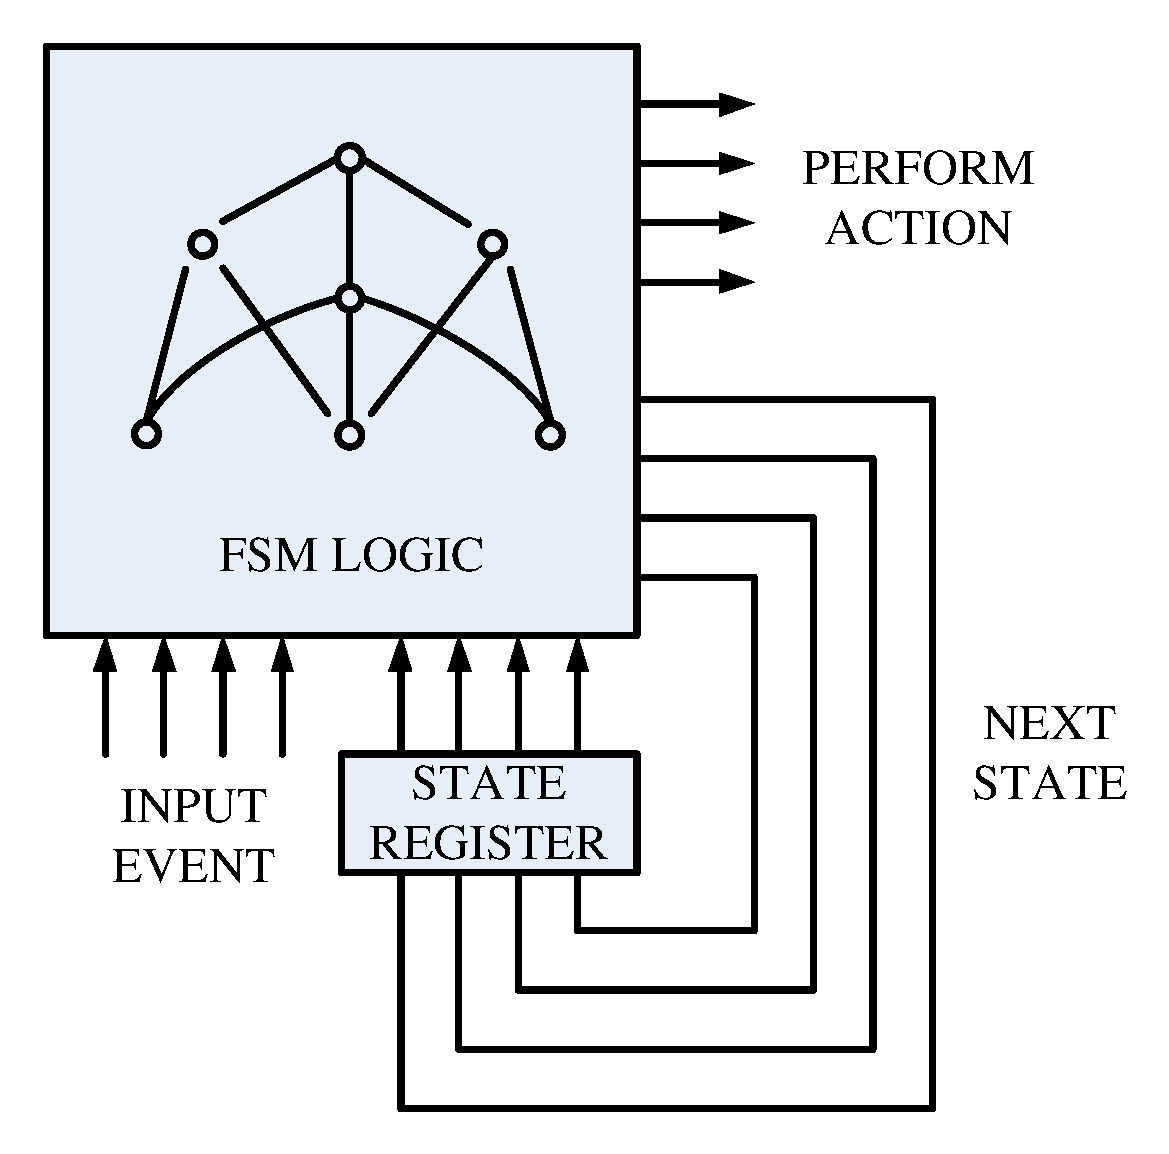
\includegraphics[width=0.5\textwidth]{files/Figures/07-FSMLogic.pdf}
  }
  \caption[Cache Controller]{Fig (a) on the left shows a high level block diagram of the cache controller's (CC) position in the memory hierarchy. The \textit{Northbridge} is used to manage data communcations between the CPU and motherboard and is also where the memory controller resides. In newer architectures such as the Intel Sandy Bridge, the \textit{Northbridge} has been integrated on chip. Fig (b) on the right depicts a cache controller where the input data path from the cache (event) is used along with the current state to perform the corresponding action and change the state of the block as required.}
  \label{fig:cache_controller_basics}
\end{figure}


The cache controller manages operations at the aligned RMAX granularity. The controller permits only one in-flight cache operation per RMAX region, i.e. transition buffer entries in the cache controller are indexed using the region bits. In-flight cache operations ensure no address overlap with stable \AB{}s in order to eliminate complex race conditions. Fig~\ref{fig:L1protocol} shows the L1 cache controller state machine for the \AC{}. 

\begin{figure}[!h]
  \centering
  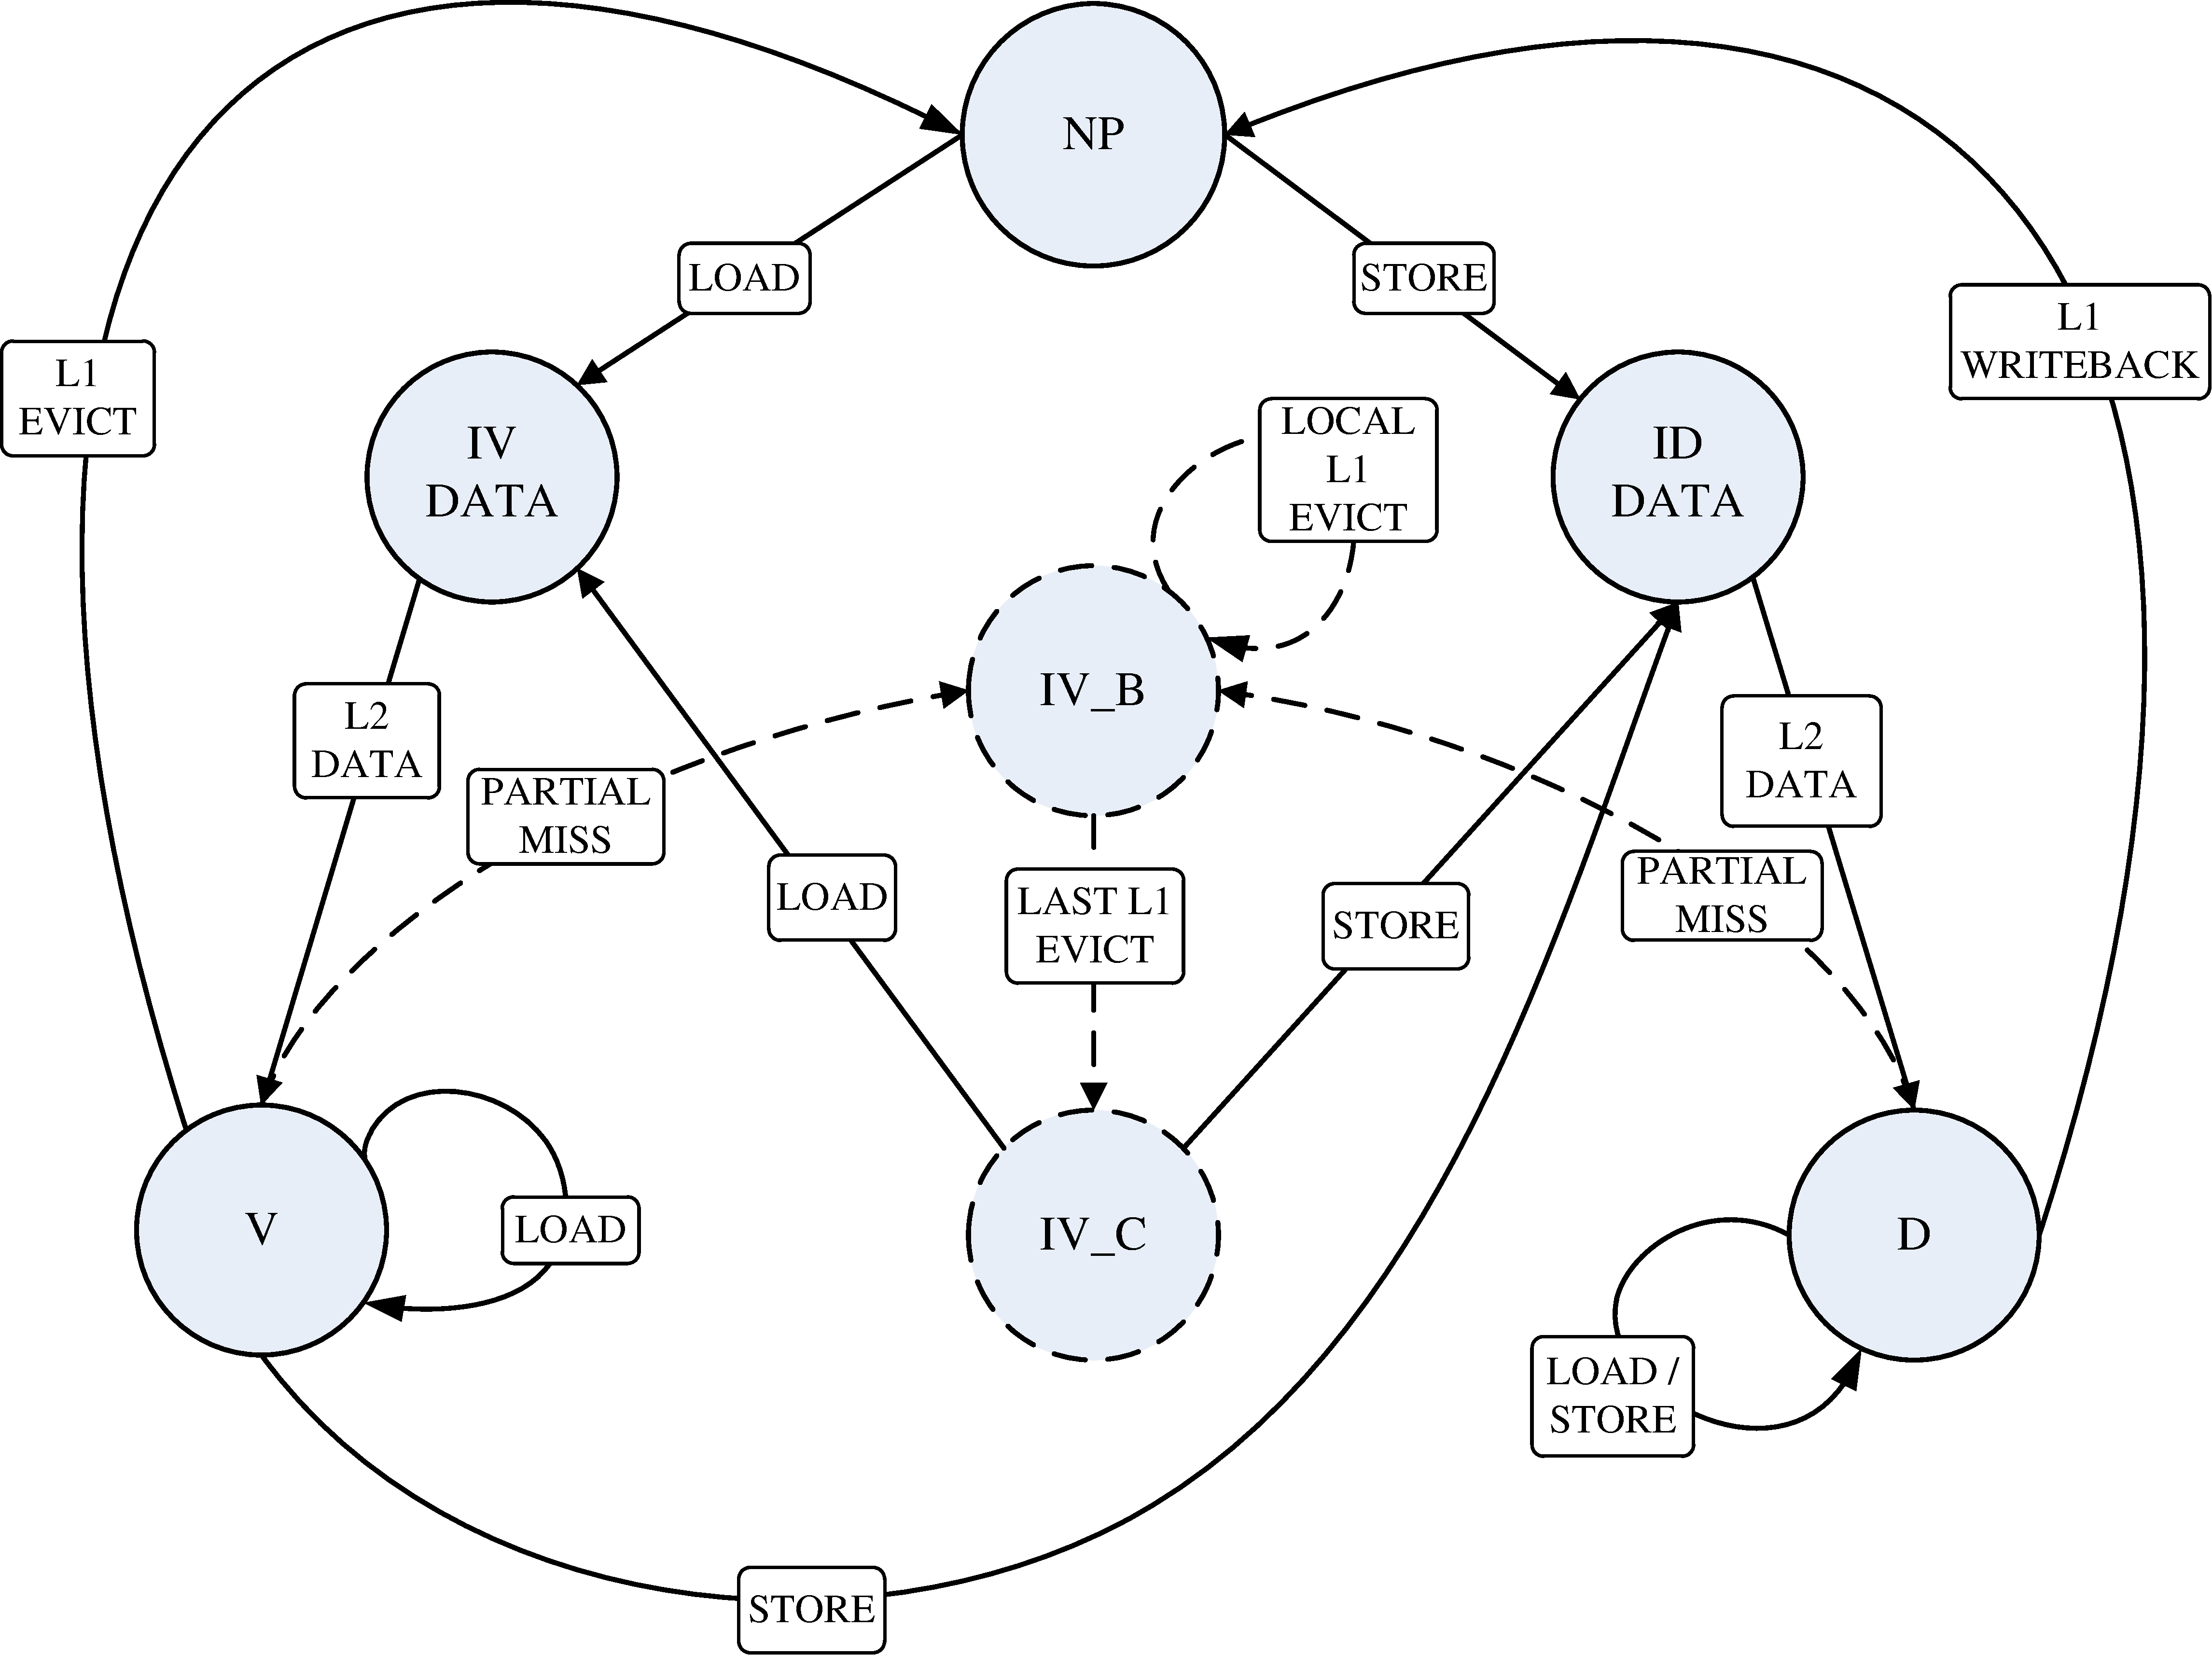
\includegraphics[width=\textwidth]{files/Figures/07-L1CC.pdf}
  \\ 
  \vspace{10pt}
  {
  \begin{tabular}{|@{~}c@{~}|@{~}p{0.75\textwidth}|} 
        
        \multicolumn{2}{c}{ \textbf{L1 cache controller states}}\\
        \hline
        State & Description \\
        \hline
        NP & \AB\ not present in the cache. \\
        \hline
        V & All words corresponding to \AB\ present and valid (read-only) \\
        \hline
        D & Valid and atleast one word in \AB\ is dirty (read-write) \\
        \hline
        {\bf IV\_B} & Partial miss being processed (blocking state) \\
        \hline
        {\bf IV\_Data} & Load miss; waiting for data from L2\\
        \hline
        ID\_Data & Store miss; waiting for data. Set dirty bit. \\
        \hline
        {\bf IV\_C} & Partial miss cleanup from cache completed (treat as full miss) \\ 
        \hline
        \multicolumn{2}{c}{}\\
        \multicolumn{2}{c}{ \textbf{ \AC\ specific events}}\\
        \hline
        \multicolumn{2}{|p{5in}|}{Partial miss: Process partial miss.} \\
        \multicolumn{2}{|p{5in}|}{Local\_L1\_Evict: Remove overlapping \AB\ to MSHR.} \\
        \multicolumn{2}{|p{5in}|}{Last\_L1\_Evict: Last \AB\ moved to MSHR. Convert to full miss and process load or store.} \\
        \hline
    \end{tabular}
    }
  \caption[L1 Cache Controller]{\textbf{L1 Cache Controller for \AC\ } : The \AC\ specific states and events are marked by dashed lines. The \AC\ specific events are described in the table.}
  \label{fig:L1protocol}
\end{figure}

\clearpage

A simple default single core protocol is assumed which contains blocks in either \code{Valid (V)}, \code{Not Present (NP)} and \code{Dirty (D)} as shown in Fig~\ref{fig:L1protocol}. There are also two transient states \code{IV Data}(block transitions from \code{Invalid/NP} to \code{Valid}, waiting for \code{Data} response from memory; cache miss caused by a load) and \code{ID Data}(block transitions from \code{Invalid/NP} to \code{Dirty}, waiting for \code{Data} response from memory; cache miss caused by a store). To handle partial misses, unique to the \AC{}, two new states are added to the default protocol, \code{IV\_B} and \code{IV\_C}. \code{IV\_B} is a blocking state that blocks other cache operations to RMAX region until all relevant \AB{}s to a partial miss are evicted. \code{IV\_C} indicates partial miss completion. This enables the controller to treat the access as a miss and issue the refill request. The \code{Partial Miss} event triggers the clean-up operations (Stage 1 and Stage 2 in Figure~\ref{fig:partial-miss}). \code{Local\_L1\_Evict} is an event that keeps being triggered for each \AB\ involved in the partial miss. \code{Last\_L1\_Evict} is triggered when the last \AB\ involved in the partial miss is evicted to the MSHR (see Stage 2 of Fig~\ref{fig:partial-miss}).

A key difference between the L1 and lower-level protocols is that the Load/Store event in the lower-level protocol may need to access data from multiple \AB{}s. In such cases, similar to the \code{Partial Miss} event, each block is read out independently before supplying the data (more details in \S~\ref{sec:multicache}).

\subsection{Area, Latency, and Energy Overhead}
\label{sec:area_latency_energy_overhead}

The extra metadata required by \AC\ are the \code{T?}(1 tag bit per word) and \code{V?}(1 valid bit per word) bitmaps as shown in Fig~\ref{fig:amoeba_cache_arch}. Table~\ref{table:overheads} shows the quantitative overhead compared to the data storage.Both the \code{T?} and \code{V?} bitmap arrays are directly proportional to the size of the cache and require a constant storage overhead (3\% in total). The \code{T?} bitmap is read in parallel with the data array and does not affect the critical path; \code{T?} adds 2\%---3.5\% (depending on cache siz) to the overall cache access energy. \code{V?}is referred only on misses when inserting a new block.

%!TEX root=/home/ska124/Dropbox/Thesis/thes-full.tex

\begin{table}[h]
{
  \centering
  
  
  {
  
    \begin{tabular}{|@{~}c@{~}|@{~}c@{~}|@{~}c@{~}|@{~}c@{~}|}
    \hline
    \multicolumn{4}{|c|}{Cache configuration}\\
    \hline
                 & 64K (256by/set) & 1MB (512by/set) & 4MB (1024by/set) \\
    \hline
    \multicolumn{4}{|l|}{Data RAM parameters} \\   
    \hline
    Delay        & 0.36ns & 2ns & 2.5 ns \\
    Energy       & 100pJ & 230pJ  & 280pJ \\
    \hline 
    \multicolumn{4}{|c|}{\AC\ components (CACTI model)} \\   
    \hline
    T?/V? map & 1KB &  16KB & 64KB \\
    Latency      & 0.019ns (5\%) & 0.12ns (6\%) & 0.2ns (6\%) \\   
    Energy       & 2pJ (2\%) & 8pJ (3.4\%) & 10pJ (3.5\%)  \\ 
    LRU  & $\frac{1}{8}$KB & 2KB & 8KB \\
    \hline
    \multicolumn{4}{|c|}{Lookup Overhead (VHDL model)} \\
    \hline
    Area    & 0.7\% & \multicolumn{2}{c|}{0.1\%} \\  
    \hline
    Latency & 0.02ns & 0.035ns & 0.04ns \\
    \hline
  \end{tabular}
  }
  \caption[Hardware Overheads]{\textbf{\AC\ hardware overheads} :  Percentage indicates overhead compared to data array of a cache. 64K cache operates in \textit{Fast mode}; 1MB and 4MB operate in \textit{Normal mode}. International Technology Roadmap for Semiconductors (ITRS) specified 32nm High Performance (HP) transistors are assumed for 64K cache and 32nm ITRS Low Output Power (LOP) transistors for 1MB and 4MB.}
  \label{table:overheads}
}
\end{table}

The \AC\ lookup logic was synthesized\footnote{Actual synthesis was at 180nm node size and the results were scaled to 32 nm (latency and energy scaled proportional to Vdd (taken from~\cite{Danowitz:2012:CDR:2133806.2133822}) and $Vdd^2$ respectively). For synthesis, we used the Synopsys design compiler (Vision Z-2007.03-SP5).} using Synopsys to quantify the area, latency and energy penalty. \AC\ is compatible with  \textit{Fast} and \textit{Normal} cache access modes~\cite{Muralimanohar:2007:ONO:1331699.1331704}, both of which read the entire set from the data array in parallel with the way selection to  achieve lower latency. \textit{Fast} mode transfers the entire set to the edge of the H-tree, while \textit{Normal} mode, only transmits the selected way over the H-tree. 

Fig~\ref{fig:ac_lookup} shows \AC\'s lookup hardware overhead on the critical path. The \AC\ lookup logic is compared against a conventional cache's lookup logic (mainly the comparators). The area overhead of the \AC\ includes registering an entire line that has been read out, the tag operation logic, and the word selector. The components on the critical path once the data is read out are the 2-way multiplexers, the $\in$ comparators, and priority encoder that selects the word; the T?  bitmap is accessed in parallel and off the critical path. \AC\ is made feasible under today's wire-limited technology where the cache latency and energy is dominated by the bit/word lines, decoder, and H-tree~\cite{Muralimanohar:2007:ONO:1331699.1331704}. \AC{}'s comparators, which operate on the entire cache set, are 6$\times$ the area of a fixed cache's comparators. In a conventional cache, the data array occupies 99\% of the overall cache area. The critical path is dominated by the wide word selector since the comparators all operate in parallel. The lookup logic adds $\simeq$ 60\% to the conventional cache's comparator time. The overall critical path is dominated by the data array access and \AC{}'s lookup circuit adds 0.02ns to the access latency and $\simeq$ 1pJ to the energy of a 64K cache, and 0.035ns to the latency and $\simeq$2pJ to the energy of a 1MB cache. 

\AC{}'s overhead needs careful consideration when implemented at the L1 cache level. There are two options for handling the latency overhead a) if the L1 cache is the critical stage in the pipeline, the CPU clock can be throttled by the latency overhead to ensure that the additional logic fits within the pipeline stage. This ensures that the number of pipeline stages for a memory access does not change with respect to a conventional cache, although all instructions bear the overhead of the reduced CPU clock; b) an extra pipeline stage can be added to the L1 hit path, adding a 1 cycle overhead to all memory accesses but ensuring no change in CPU frequency. The performance impact of both approaches is quantified in \S~\ref{sec:evaluation}.


\subsection{Tag-only Operations}  

Conventional caches support tag-only operations to reduce data port contention. While the \AC\ merges tags and data, like many commercial processors it decouples the replacement metadata and valid bits from the tags, accessing the tags only on cache lookup. Lookups can be either CPU side or network side (coherence invalidation and Writeback/Forwarding). CPU-side lookups and writebacks ($\simeq$ 95\% of cache operations) both need data and hence \AC\ in the common case does not introduce extra overhead. \AC\ does read out the entire data array unlike serial-mode caches as discussed previously. Invalidation checks and snoops can be more energy expensive with \AC{} compared to a conventional cache. Fortunately, coherence snoops are not common in many applications (e.g., 1/100 cache operations in SpecJBB) as a coherence directory and an inclusive LLC filter them out.


\subsection{Tradeoff with large caches} 
\label{sec:tradeoff_with_large_caches} % formerly extensions

\begin{figure}[h] 
\centering
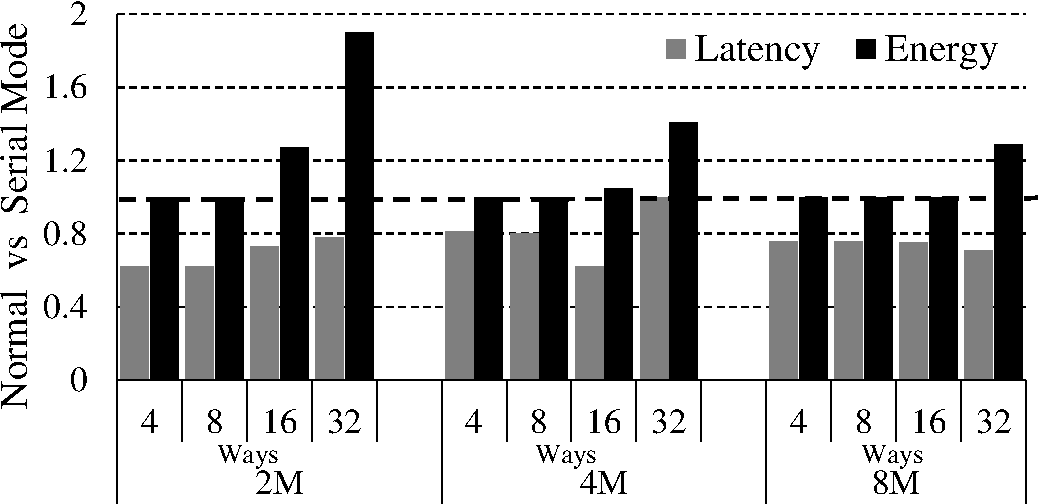
\includegraphics[width=0.7\textwidth]{files/Plots/07-Serial_vs_Normal.pdf}

Baseline: Serial. $\leq1$ Normal is better.  32nm, ITRS  LOP. 
\caption[Serial vs. Normal - Latency and Energy]{\textbf{Serial vs Normal mode cache} : }
\label{fig:serial_normal_graph} 
\end{figure}

Large caches with many words per set ($\equiv$ highly associative conventional cache) need careful consideration. Typically, highly associative caches tend to serialize tag and data access with only the relevant cache block read out on a hit and no data access on a miss. The tradeoff between reading the entire set (normal mode), which is compatible with \AC{}, and only the relevant block (serial mode), is analysed herein. The cache size is varied from 2M---8M and associativity from 4(256B/set) --- 32 (2048B/set).  Under current technology constraints (Figure~\ref{fig:serial_normal_graph}), only at very high associativity does serial mode demonstrate a notable energy benefit. Large caches are dominated by H-tree energy consumption and reading out the entire set at each sub-bank imposes an energy penalty when bitlines and wordlines dominate (2KB+ number of words per set).

\begin{table}[h]
\begin{center}
\begin{tabular}{|c|c|c|c|c|c|c|}
\hline
  &  \multicolumn{2}{c|} {64K (256 bytes/set)} 
  &  \multicolumn{2}{c|} {1MB (512 bytes/set)} 
  & \multicolumn{2}{c|} {2MB (1024 bytes/set)} \\
\hline
N Tags/set & 2 & 4 & 4 & 8 & 8 & 16 \\
Overhead &  1KB & 2KB  & 2KB & 16KB  & 16KB & 32KB  \\  
\hline
\multicolumn{7}{|l|} {Benchmarks} \\
\hline
Low      & 30\% & 45\% & 42\% & 64\% & 55\% & 74\%\\
Moderate & 24\% & 62\% & 46\% & 70\% & 63\% & 85\%\\
High     & 35\% & 79\% & 67\% & 95\% & 75\% & 96\%\\
\hline
\end{tabular}
\caption[Fast Tag accesses percent]{Percentage of direct accesses with fast tags}
\label{fig:tagcount}

\end{center}
\end{table}


\AC\ can be tuned to minimize the hardware overhead for large caches. With many words/set the cache utilization improves due to longer block lifetimes making it feasible to support \AB{}s with a larger minimum granularity ($>$ 1 word). If we increase minimum granularity to two or four words, only every third or fifth word could be a tag, meaning the number of comparators and multiplexers reduce to $\frac{N_{words/set}}{3}$ or $\frac{N_{words/set}}{5}$. When the minimum granularity is equal to max granularity (RMAX), we obtain a fixed granularity cache with $N_{words/set}/RMAX$ ways. Cache organizations that collocate all the tags together at the head of the data array enable tag-only operations and serial \AB\ accesses that need to activate only a portion of the data array. However, the set may need to be compacted at each insertion. Recently, Loh and Hill~\cite{Loh:2012:SVL:2311639.2311823} explored such an organization for supporting tags in multi-gigabyte caches.


The use of \textit{Fast Tags} help reduce the tag lookups in the data array. Fast tags use a separate traditional tag array-like structure to cache the tags of the recently-used blocks and provide a pointer directly to
the \AB{} similar to \textit{Indirect Index Caches}(see \S~\ref{sec:indirect_index_caches}). The number of \textit{Fast Tags} needed per set is proportional to the number of blocks in each set, which varies with the spatial locality in the application and the number of bytes per set (more details in Section~\ref{sec:efficiency}). Three different cache configurations were studied (64K 256B/set, 1M 512B/set, and 2M 1024B/set) while varying the number of fast tags per set (see Table~\ref{fig:tagcount}). With 8 tags/set (16KB overhead), the fast tags can filter 64---95\% of the accesses in a 1MB cache and 55---75\% of the accesses in a 2MB cache.

\subsection{Multi-level Caches}
\label{sec:multicache}

We discuss the design of inclusive cache hierarchies including multiple \AC{}s; we illustrate using a 2-level hierarchy. Inclusion means that the L2 cache contains a superset of the data words in the L1 cache; however, the two levels may include different granularity blocks. For example, the Sun Niagara T2 uses 16 byte L1 blocks and 64 byte L2 blocks. \AC\ permits non-aligned blocks of variable granularity at the L1 and the L2, and needs to deal with two issues: a) L2 recalls that may invalidate multiple L1 blocks and b) L1 refills that may need data from multiple blocks at the L2. For both cases, we need to identify all the relevant \AB{}s that overlap with either the recall or the refill request. This situation is similar to a Nigara's L2 eviction which may need to recall 4 L1 blocks. \AC{}'s logic ensures that all \AB{}s from a region map to a single set at any level (using the same RMAX for both L1 and L2). This ensures that L2 recalls or L1 refills index into only a single set. To process multiple blocks for a single cache operation, we use the step-by-step process outlined in Section~\ref{sec:partialmiss} (\spot{1} and \spot{2} in Figure~\ref{fig:partial-miss}). Finally, the L1-L2 interconnect needs 3 virtual networks, two of which, the L2$\rightarrow$L1 data virtual network and the L1$\rightarrow$L2 writeback virtual network, can have packets of variable granularity; each packet is broken down into a variable number of smaller physical flits.


\subsection{Cache Coherence}
\label{sec:coherence}

There are three main challenges that variable cache line granularity introduces when interacting with the coherence protocol: 1) How is the coherence directory maintained? 2) How to support variable granularity read sharing? and 3) that is the granularity of write invalidations? The key insight that ensures compatibility with a conventional
fixed-granularity coherence protocol is that a \AB\ always lies within an aligned RMAX byte region (see \S~\ref{sec:architecture}). To ensure correctness, it is sufficient to maintain the coherence granularity and directory information at a fixed granularity $\leq$ RMAX granularity. Multiple cores can simultaneously cache any variable granularity \AB\ from the same region in \textit{S}hared state; all such cores are marked as sharers in the directory entry. A core that desires exclusive ownership of an \AB\ in the region uses the directory entry to invalidate every \AB\ corresponding to the fixed coherence granularity. All \AB{}s relevant to an invalidation   will be found in the same set in the private cache (see set indexing in \S~\ref{sec:architecture}). The coherence granularity could potentially be $<$ RMAX so that false sharing is not introduced in the quest  for higher cache utilization (larger RMAX). The core claiming the ownership on a write will itself fetch only the desired granularity \AB{}, saving bandwidth. A detailed evaluation of the coherence protocol is beyond the scope of the current paper.

\section{Simulation Infrastructure}

% \section{Application Traces}
% \subsection{Intel Pin}
% \subsection{Generating a memory access trace}
% \subsection{Workload selection}
% \section{GEMS Infrastructure}
% \subsection{Introduction}
% \subsection{Components}
% \subsection{SLICC}
% \subsection{Amoeba-Single Protocol}

%!TEX root=/home/ska124/Dropbox/Thesis/thes-full.tex

%%%%%%%%%%%%%%%%%%%%%%%%%%%%%%%%%%%%%%%%%%%%%%%%%
%
%     Chapter 5
%
%%%%%%%%%%%%%%%%%%%%%%%%%%%%%%%%%%%%%%%%%%%%%%%%

\chapter{Evaluation}
\label{chap:evaluation}
This chapter evaluates the performance of the \AC\ described in Chapter~\ref{chap:ac_architecture}. The evaluation is performed using the infrastructure described in Chapter~\ref{sec:simulation_infrastructure}. This chapter is divided into sections based on performance evaluations of:
\begin{itemize}[noitemsep]
	\item Comparison against a fixed granularity cache
	\item Adaptivity of the \AC\
	\item The spatial pattern predictor
	\item \AC\ versus other approaches
\end{itemize}

\section{Improved Memory Hierarchy Efficiency}
\label{sec:efficiency}
\vspace{5pt}
\noindent \textbf{Result 1:}{\emph~{\AC\ increases cache capacity by harvesting
  space from unused words and can achieve an 18\% reduction in both L1 and
  L2 miss rate.}
\\ \\
\noindent \textbf{Result 2:}{\emph~{\AC\ adaptively sizes the cache block
  granularity and reduces L1$\leftrightarrow$L2 bandwidth by 46\% and
  L2$\leftrightarrow$Memory bandwidth by 38\%.}
}
\\ \\
In this section, the bandwidth and miss rate properties of an \AC\ are compared against a conventional cache. A \textit{Fixed} cache represents a conventional cache which allocates a fixed granularity cache block on a refill request. The accuracy of the spatial pattern predictor is an important factor which governs the accuracy of the \AC\ and is evaluated separately. For the results presented in this section, cache line utilization statistics, gathered from a prior run of the application on a conventional cache, are used to drive the predictor. This isolates the benefits of the \AC\ from the potentially changing accuracy of the spatial pattern predictor across different cache geometries. This also ensures that the spatial granularity predictions can be replayed across multiple simulation runs. To ensure equivalent data storage space, the \AC\ size is set to the sum of the tag array and the data array in a conventional cache. At the L1 level (64K), the net capacity of the \AC\ is 64K + 8*4*256 bytes and at the L2 level (1M) configuration, it is 1M + 8*8*2048 bytes. The L1 cache has 256 sets and the L2 cache has 2048 sets. 

Fig~\ref{fig:eval_scatter_bw_64k_1m} plots the miss rate and the traffic characteristics of the \AC{}.  Since \AC{} can hold blocks varying in size from 8B to 64B, each set can hold more blocks by utilizing the space saved from eliminating untouched words. The \AC\ reduces the 64K L1 miss rate on average by 23\%\footnote{All reported averages are geometric mean unless otherwise specified.} and standard deviation(SD) of 24 for the Low group, and by 21\%(SD:16) for the moderate group; even applications with high spatial locality experience a 7\%(SD:8) improvement in miss rate. There is a 46\%(SD:20) reduction on average in L1$\leftrightarrow$L2 bandwidth. At the 1M L2 level, the \AC\ improves the moderate group's miss rate by 8\%(SD:10) and bandwidth by 23\%(SD:12).  Applications with moderate utilization make better use of the space harvested from unused words by \AC{}. Many low utilization applications tend to be streaming and providing extra cache space does not help lower miss rate. However, by not fetching unused words, the \AC\ achieves a significant reduction (38\%(SD:24) on average) in off-chip L2$\leftrightarrow$Memory bandwidth; even High utilization applications see a 17\%(SD:15) reduction in bandwidth.  Utilization and miss rate are not, however, always directly correlated (more details in \S~\ref{sec:adaptivity}).

With the \AC\, the number of blocks per set varies based on the granularity of the blocks being fetched, which in turn depends on the spatial locality in the application. Table~\ref{table:blockcount} shows the average number of blocks per set. In applications with low spatial locality, the \AC\ adjusts the block size and adapts to store many smaller blocks. The 64K L1 \AC\ stores 10 blocks per set for mcf and 12 blocks per set for art, effectively increasing associativity without introducing hardware overheads. At the L2, when the working set starts to fit in the L2 cache, the set is partitioned into fewer blocks. 

\begin{figure}[ht]

  \subfloat[64K - Low]{
    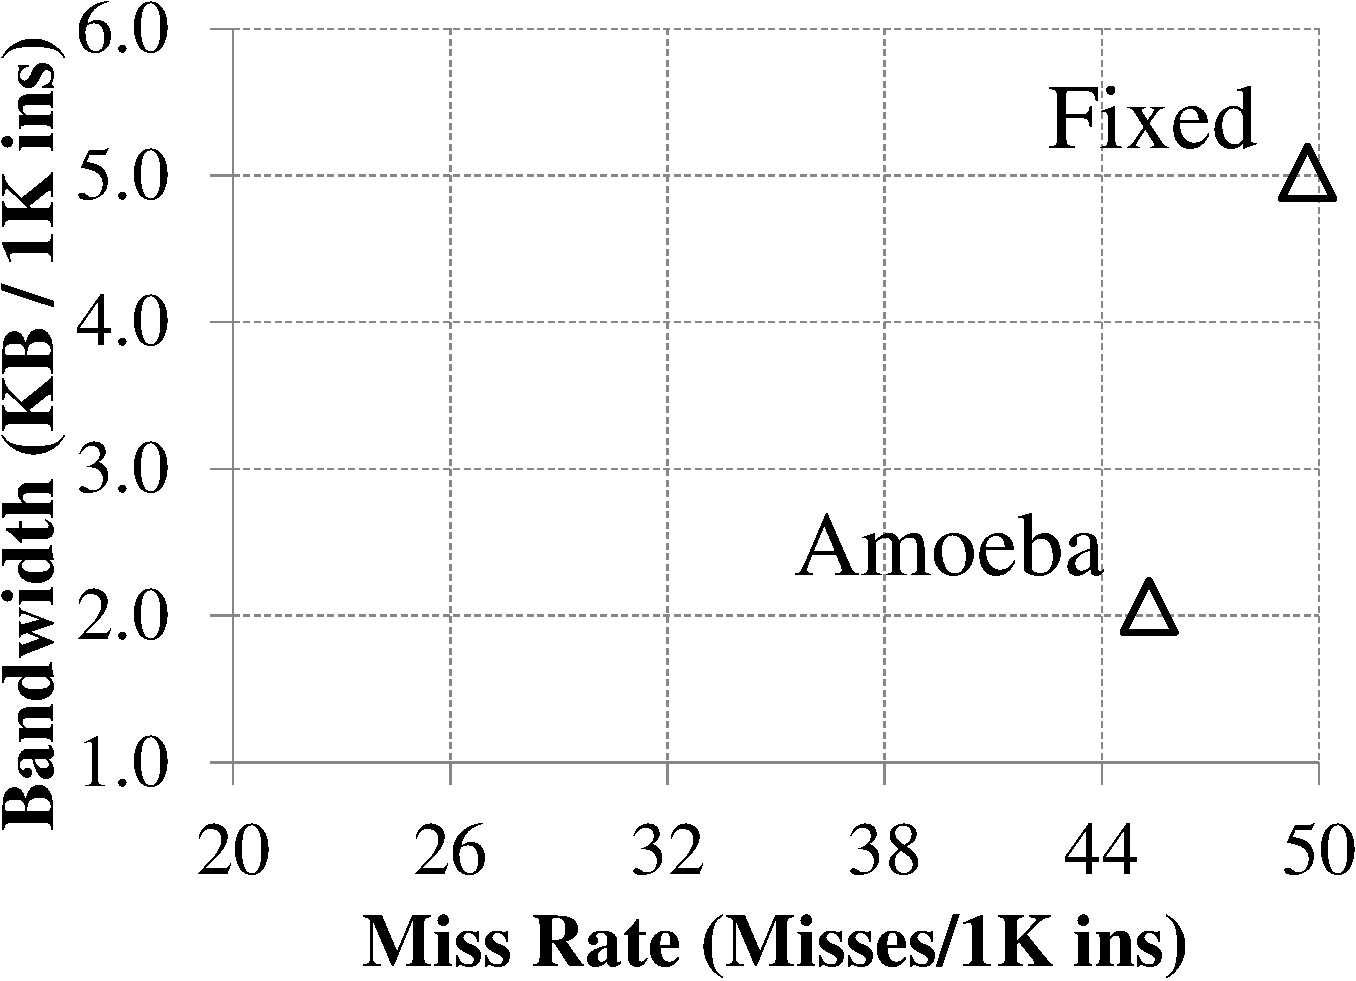
\includegraphics[width=0.48\textwidth]{files/Plots/08-Scatter_Bw_Miss_64K_low.pdf}
  }
  \subfloat[1M - Low]{
     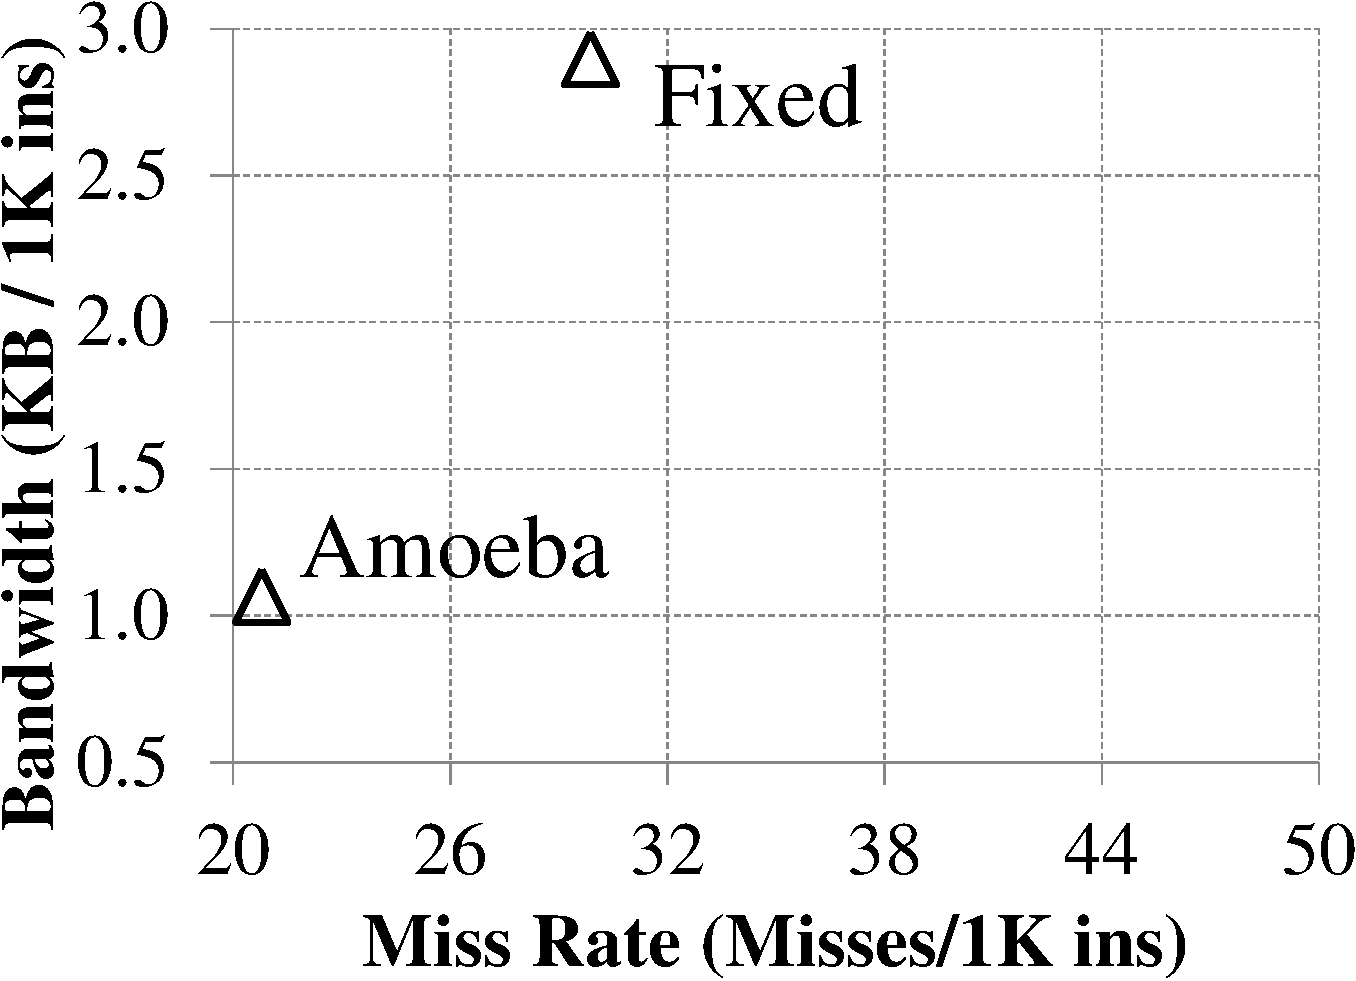
\includegraphics[width=0.48\textwidth]{files/Plots/08-Scatter_Bw_Miss_1M_low.pdf}
  }
  
  \subfloat[64K - Moderate]{
    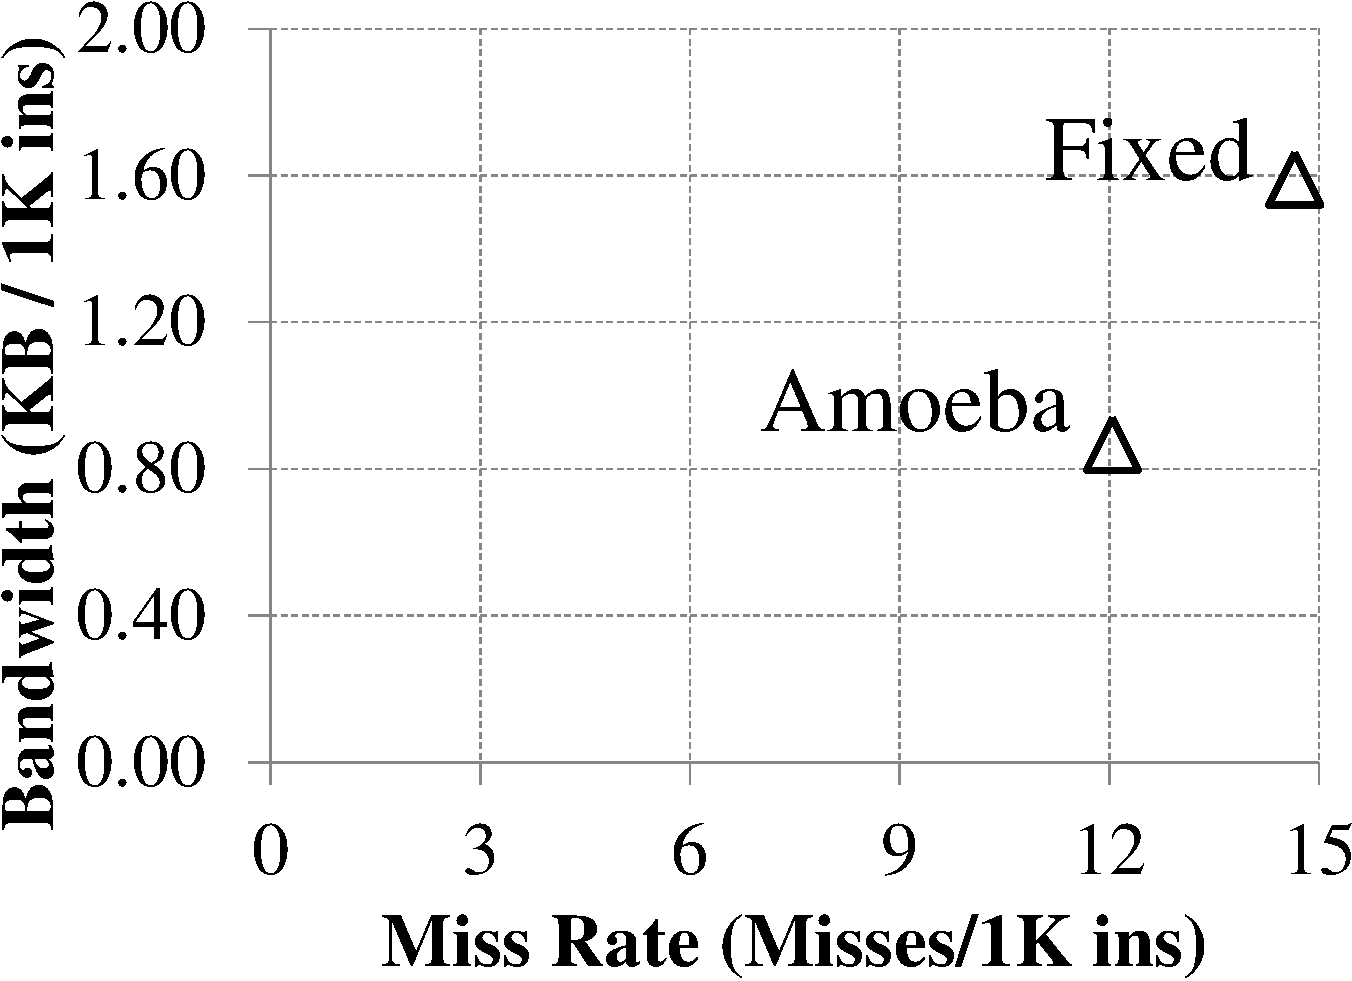
\includegraphics[width=0.48\textwidth]{files/Plots/08-Scatter_Bw_Miss_64K_mod.pdf}
  }
  \subfloat[1M - Moderate]{
     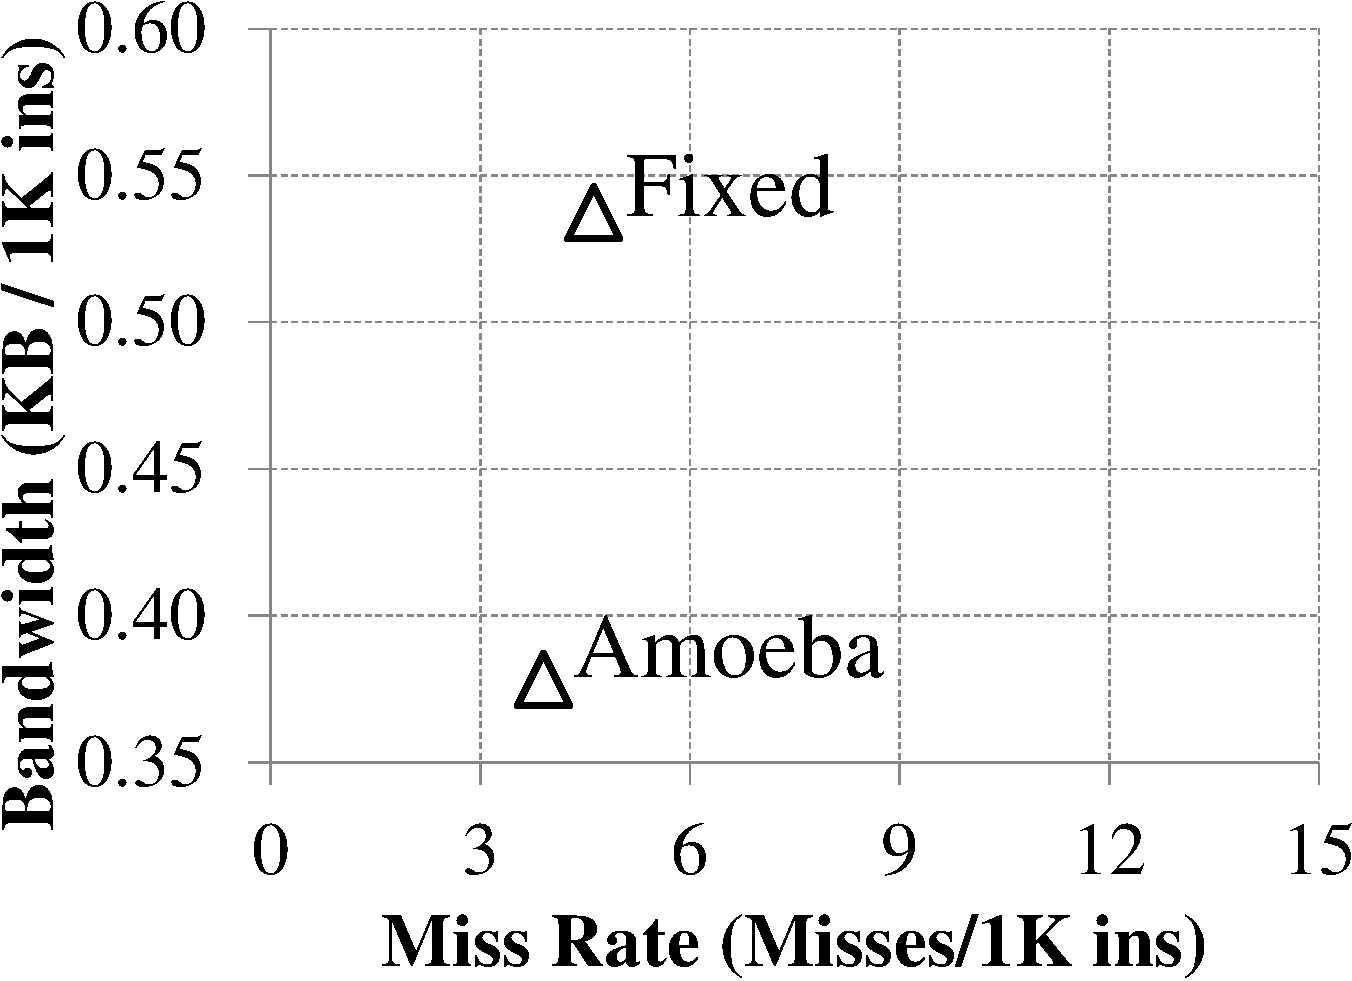
\includegraphics[width=0.48\textwidth]{files/Plots/08-Scatter_Bw_Miss_1M_mod.pdf}
  }
    
  \subfloat[64K - High]{
    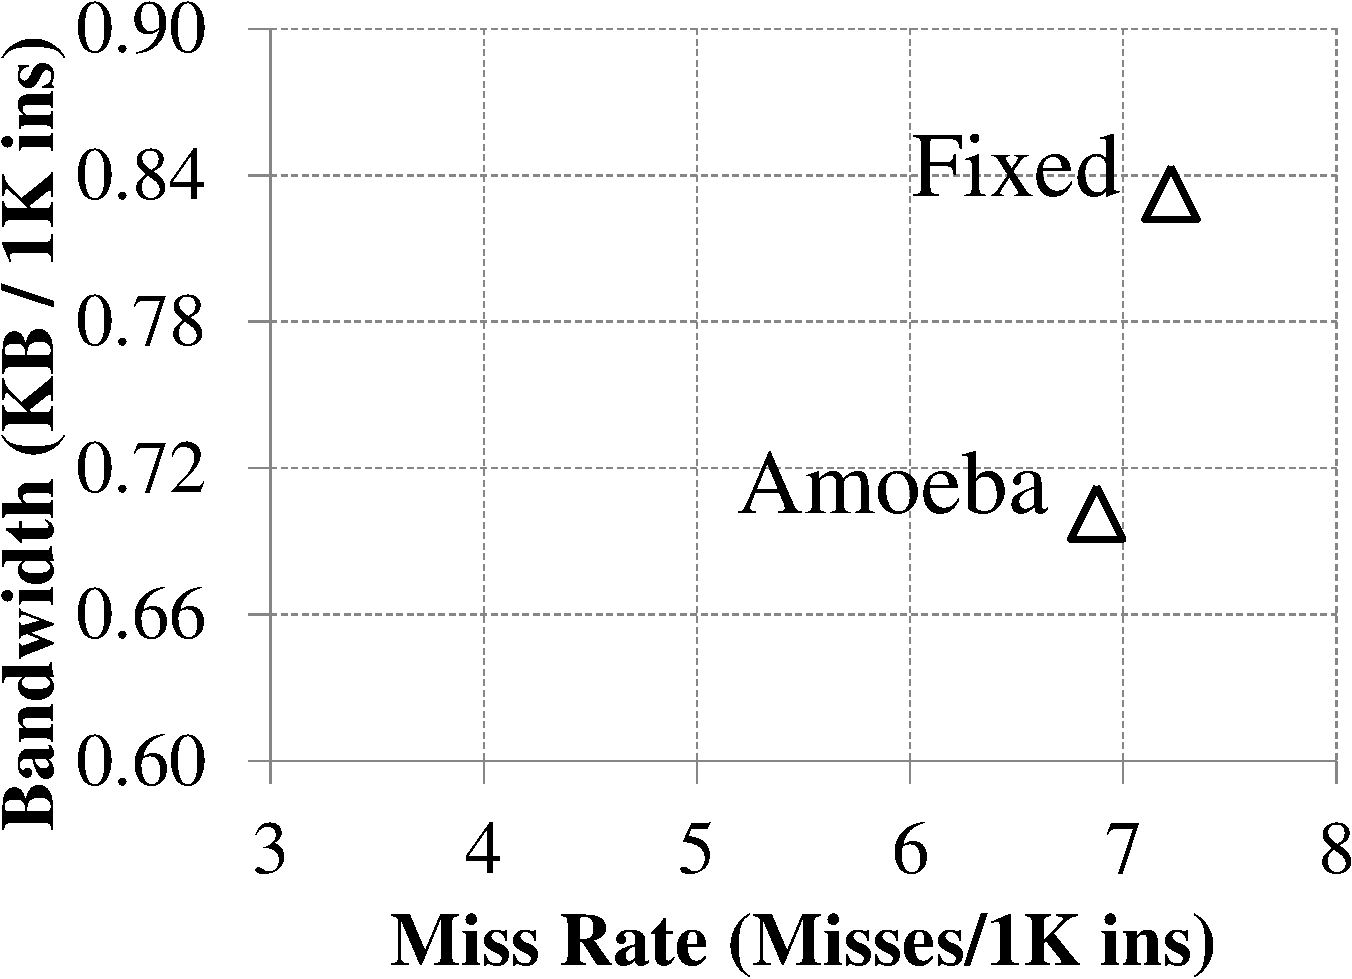
\includegraphics[width=0.48\textwidth]{files/Plots/08-Scatter_Bw_Miss_64K_high.pdf}
  }
  \subfloat[1M - High]{
     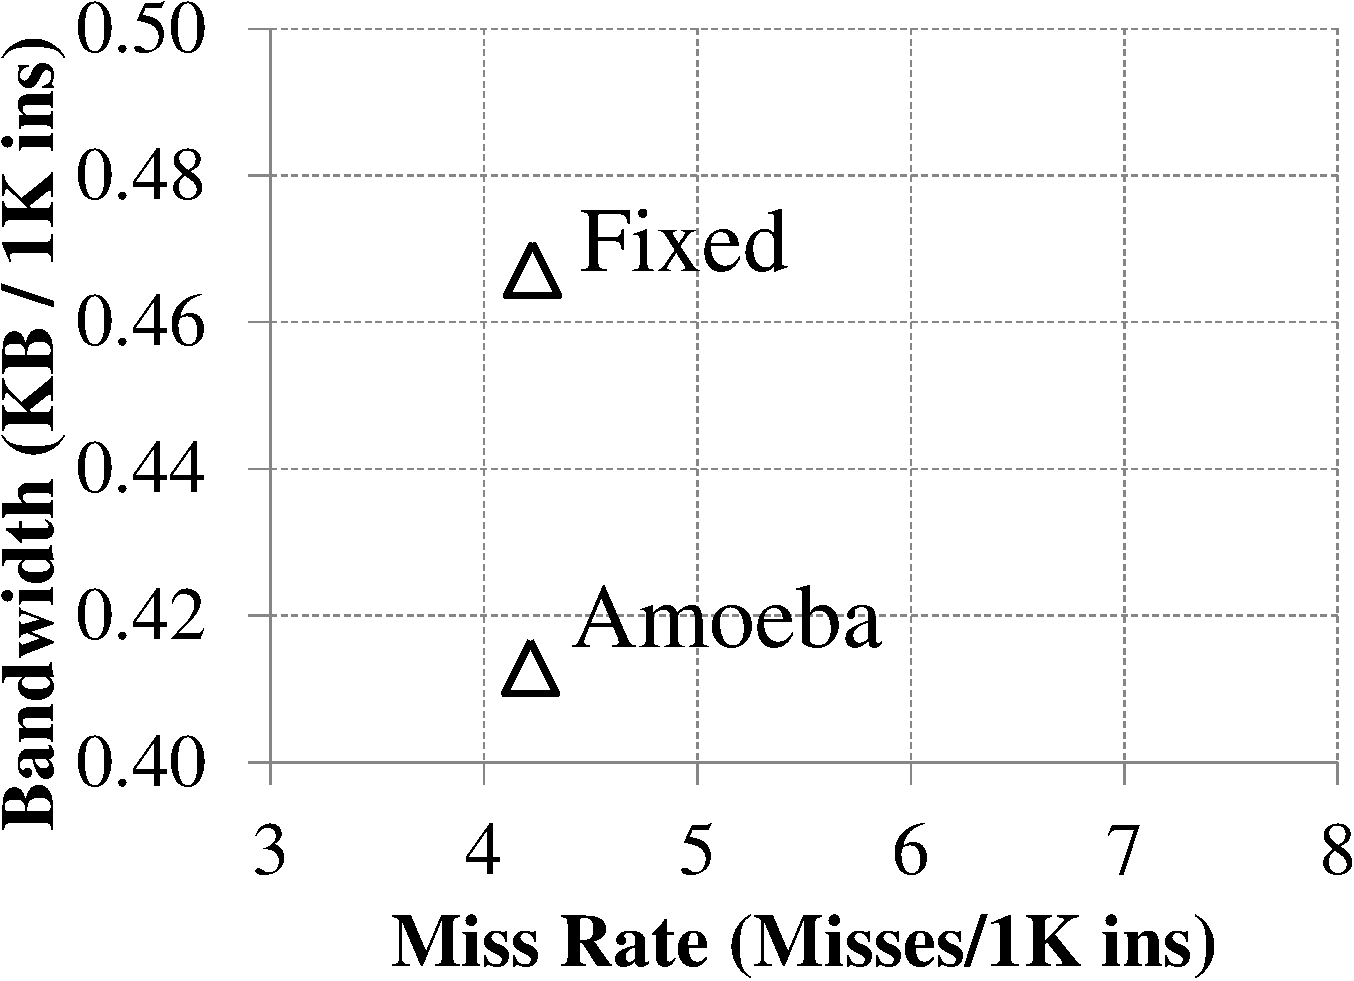
\includegraphics[width=0.48\textwidth]{files/Plots/08-Scatter_Bw_Miss_1M_high.pdf}
  }

  \caption[Bandwidth vs. Miss Rate]{Bandwidth vs. Miss Rate for a fixed granularity cache and \AC{}. (a),(c),(e): 64K, 4-wayL1 equivalent (b),(d),(f): 1M, 8-way LLC equivalent.  Markers on the plot indicate cache block size. Note the different scales for different groups.}
  \label{fig:eval_scatter_bw_64k_1m}
\end{figure}

\clearpage

%!TEX root=/home/ska124/Dropbox/Thesis/thes-full.tex
\begin{table}[h]
  \centering
  \begin{tabular}{|c|c|}
  \hline 
    Blocks/Set & 64K Cache, 288 B/set \\
    \hline
    4---5  &  ferret, cactus, firefox, eclipse, facesim, freqmine, milc, astar\\
    6---7  &  tpc-c, tradesoap, soplex, apache, fluidanimate\\
    8---9  &  h2, canneal, omnetpp, twolf, x264, lbm, jbb \\
    10---12 & mcf, art \\
    \hline
    \multicolumn{2}{c}{} \\
    \hline
    Blocks/Set & 1M Cache, 576 B/set \\
    \hline
    3---5 & eclipse, omnetpp   \\
    8---9 & cactus, firefox, tradesoap, freqmine, h2, x264, tpc-c   \\
    10---11  & facesim, soplex, astar, milc, apache, ferret  \\
    12---13  & twolf, art, jbb, lbm , fluidanimate \\
    15---18 & canneal, mcf \\
    \hline
  \end{tabular}
  \caption[Amoeba Blocks per set]{Average number of \AB{}s per set}
  \label{table:blockcount}
\end{table}


Note that applications like eclipse and omnetpp hold only 3---5 blocks per set on average (lower than conventional associativity) due to their low miss rates (see Table~\ref{table:Abs_Eval_Oracle}). With streaming applications (e.g., canneal), \AC\ increases the number of blocks/set to $>$15 on average. Finally, some applications like apache store between 6---7 blocks/set with a 64K cache with varied block sizes (see Figure~\ref{fig:StackBar_PredictorSize}): approximately 50\% of the blocks store 1-2 words and 30\% of the blocks store 8 words at the L1. As the size of the cache increases and thereby the lifetime of the blocks, the \AC\ adapts to store larger size blocks as can be seen in Figure~\ref{fig:StackBar_PredictorSize}.
\\ \\
\indent Utilization is improved greatly across all applications (90\%+ in many cases). Figure~\ref{fig:StackBar_PredictorSize} shows the distribution of cache block granularities in \AC{}. The \AB\ distribution matches the word access distribution presented in Fig~\ref{fig:stackbar_words_64k}). With the 1M cache, the larger cache size improves block lifespan and thereby utilization, with a significant drop in the \% of 1---2 word blocks. However, in many applications (tpc-c, apache, firefox, twolf, lbm, mcf), up to 20\% of the blocks are 3--6 words wide, indicating the benefits of adaptivity and the challenges faced by a fixed granularity conventional cache.

\begin{figure}[!h]
  \centering
  \subfloat[64K L1 cache]{
    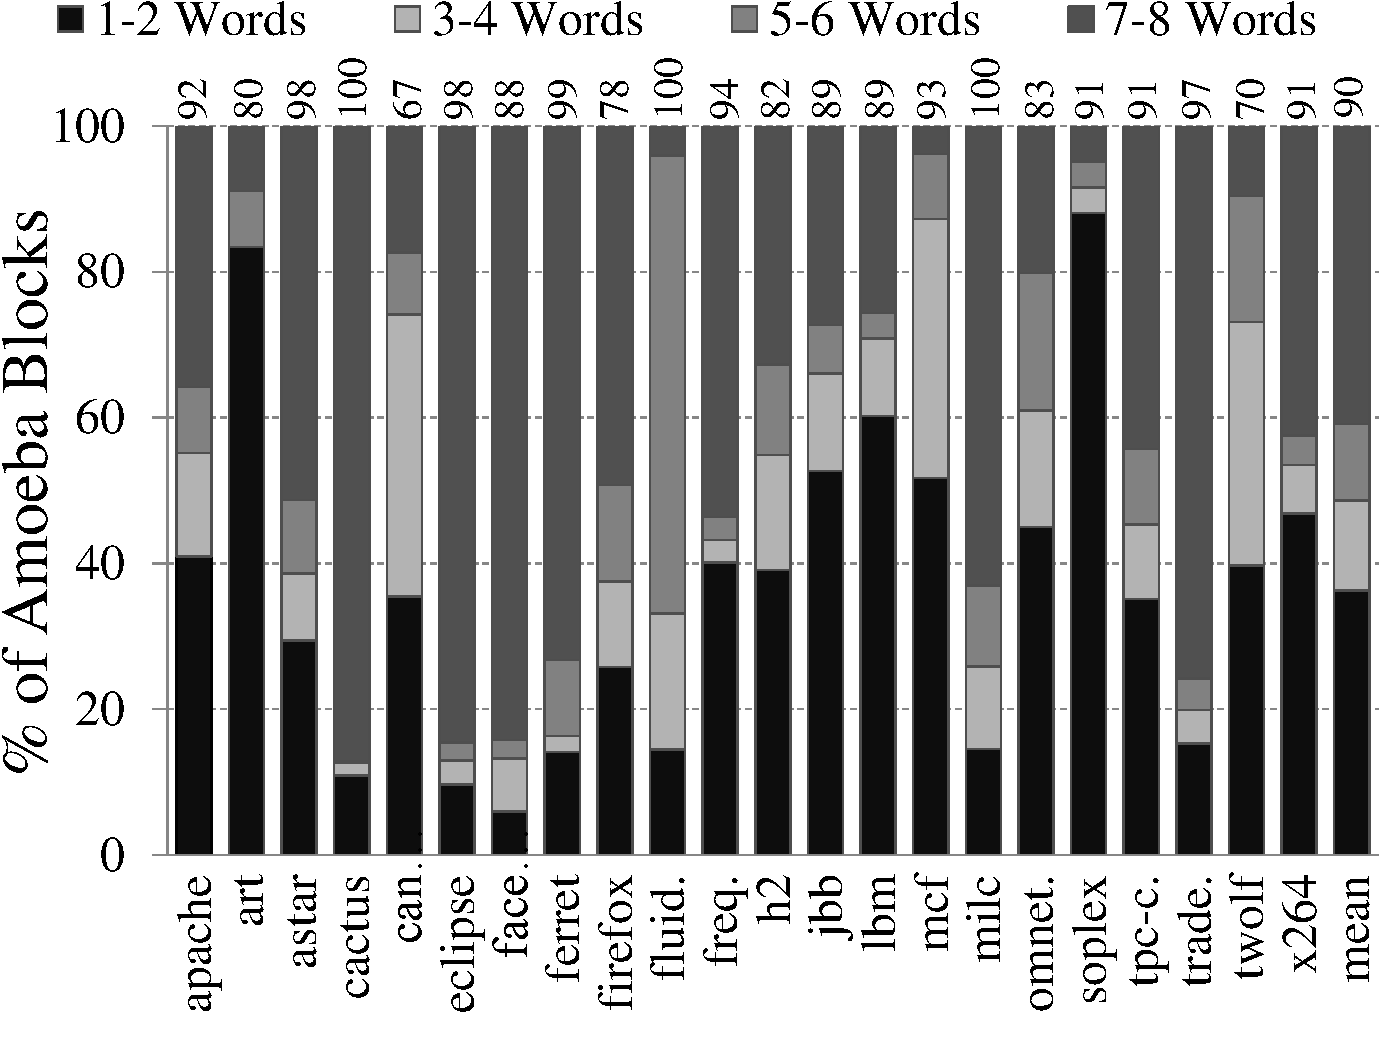
\includegraphics[width=0.8\textwidth]{files/Plots/08-StackBar_PredictSize_64K.pdf}
  }

  \subfloat[1M L2 cache]{
    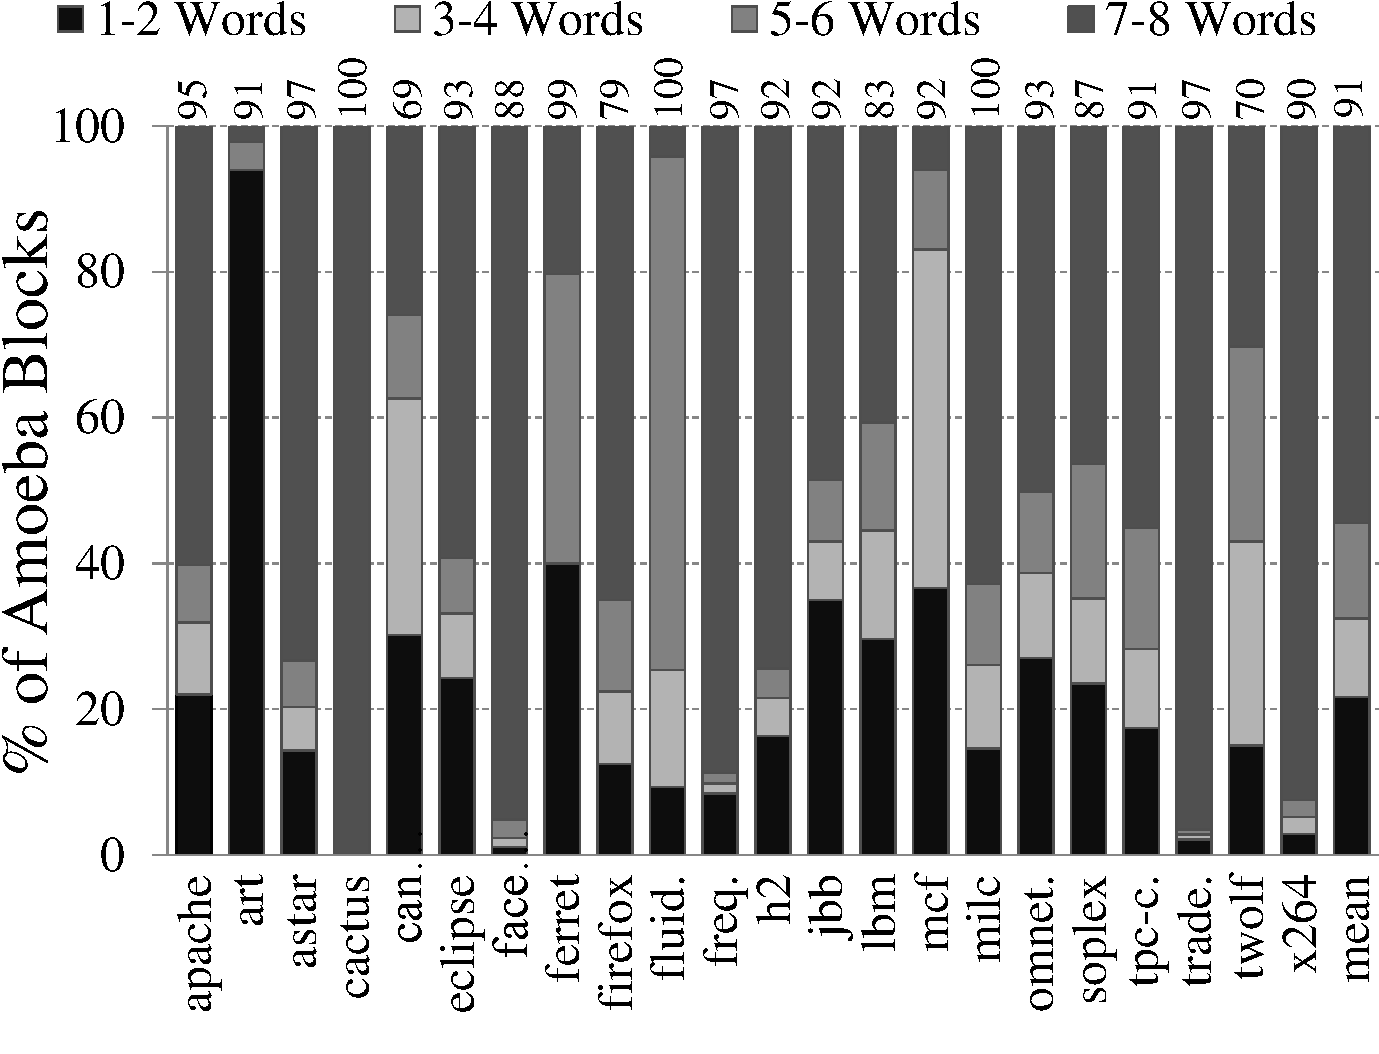
\includegraphics[width=0.8\textwidth]{files/Plots/08-StackBar_PredictSize_1M.pdf}
  }
  \caption[Distribution of cache block sizes]{Distribution of cache line granularities in the (a) 64K L1 and (b) 1M L2 \AC{}. Average utilization is on top.}
  \label{fig:StackBar_PredictorSize}
\end{figure}

\clearpage

\begin{figure}[!h]
  \centering
  \subfloat[64K L1 cache]{
    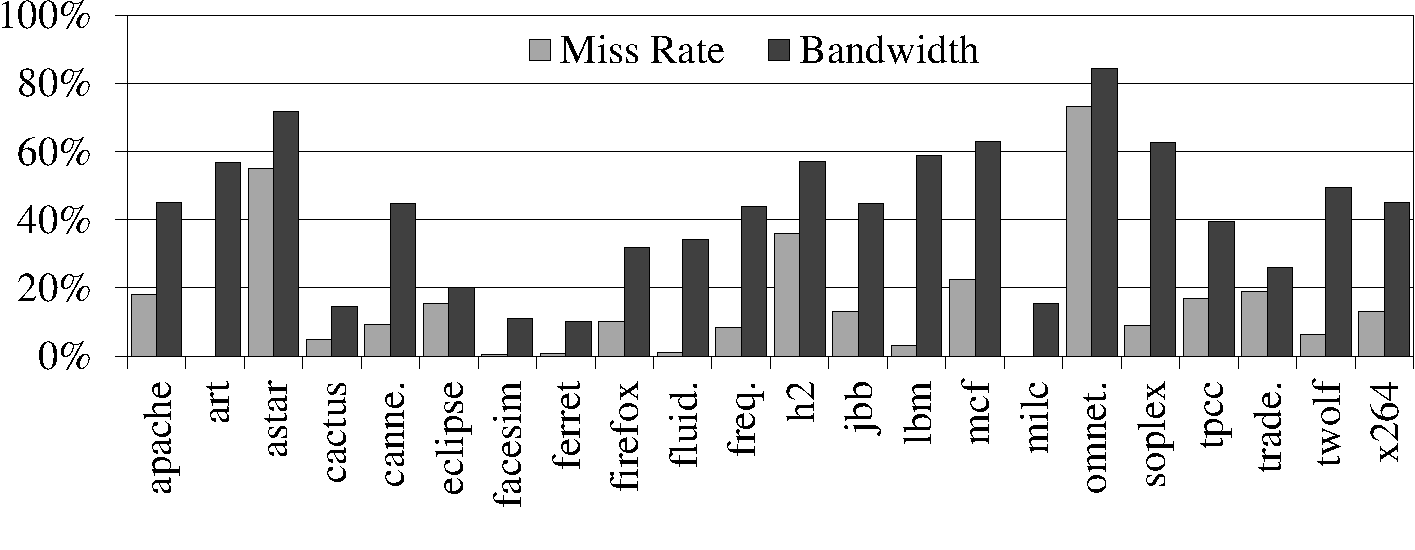
\includegraphics[width=\textwidth]{files/Plots/08-Oracle-64K-Miss-BW-Improvement.pdf}
  }

  \subfloat[1M L2 cache]{
    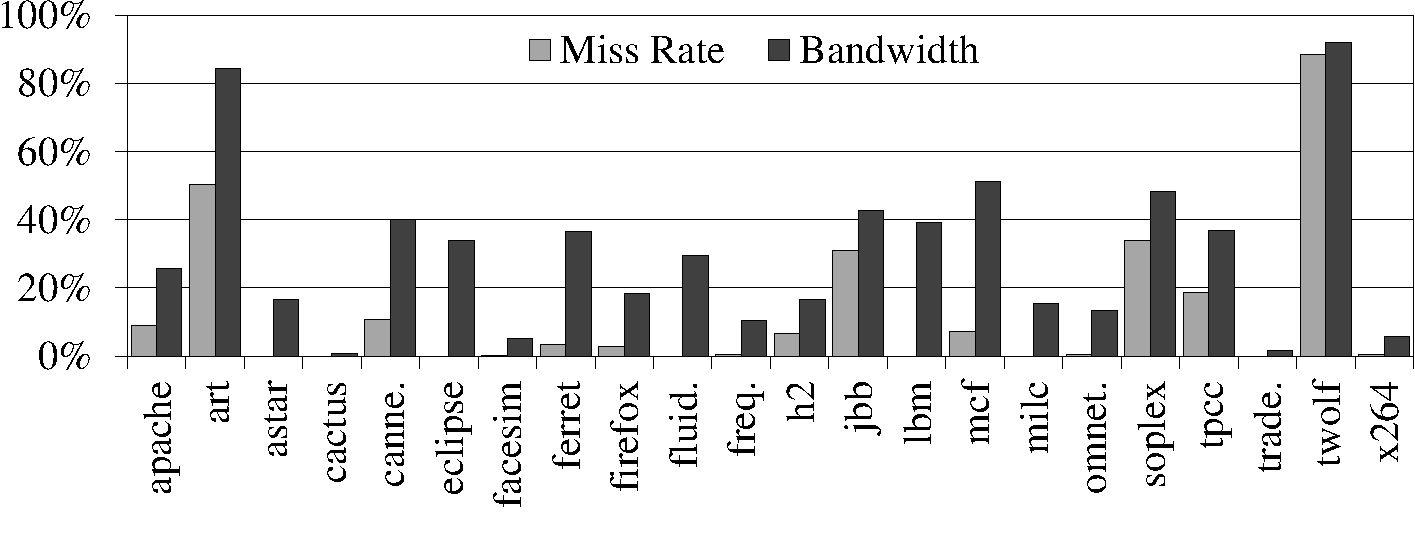
\includegraphics[width=\textwidth]{files/Plots/08-Oracle-1M-Miss-BW-Improvement.pdf}
  }
  \caption[Miss Rate and Bandwidth Improvement]{Miss Rate and bandwidth reduction with respect to a fixed granularity conventional cache with cache line size 64 bytes for (a) 64K equivalent \AC\ and (b) 1M equivalent \AC{}.}
  \label{fig:miss_bw_reduction}
\end{figure}

\section{Overall Performance and Energy}
\label{sec:overall_performance_and_energy}
\noindent \textbf{Result 3:}{~\AC\ improves overall cache efficiency and boosts performance by 10\% on commercial applications\footnote{``Commercial'' applications includes Apache, SpecJBB and TPC-C.}, saving up to 11\% of the energy of the on-chip memory hierarchy. Off-chip L2$\leftrightarrow$memory energy sees a mean reduction of 41\% across all workloads. 

\begin{figure}[!h]
  \centering
    \subfloat[Energy Improvement]{
      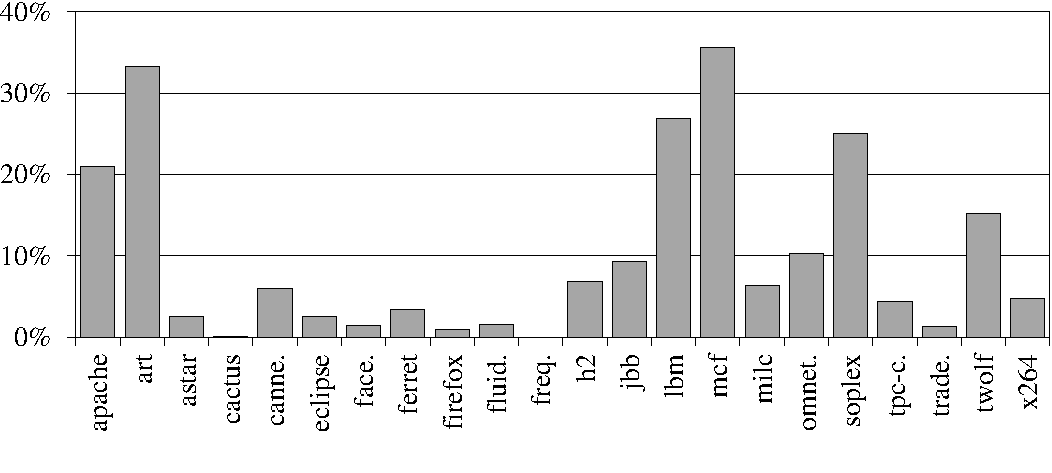
\includegraphics[width=\textwidth]{files/Plots/08-Oracle_Energy.pdf}
    }
    
    \subfloat[Performance Improvement]{
      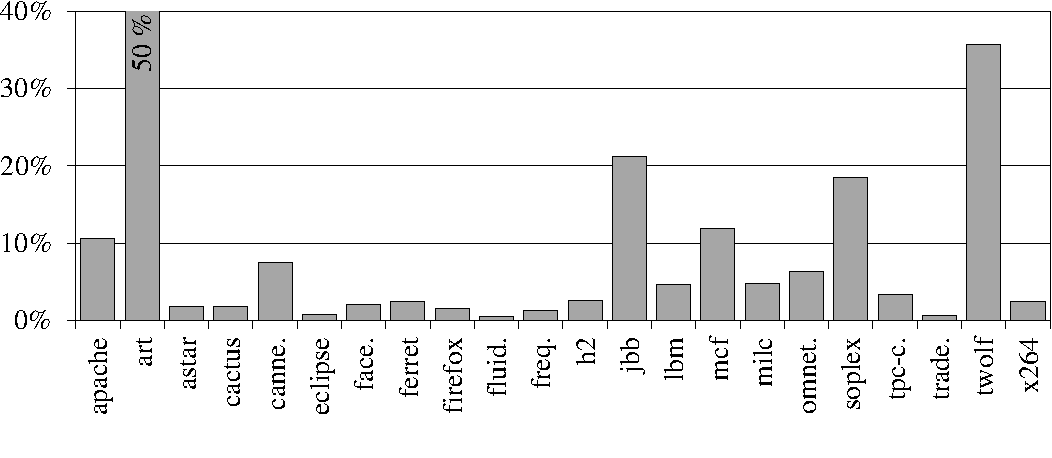
\includegraphics[width=\textwidth]{files/Plots/08-Oracle_Perf.pdf}
    }
    \caption[Overall performance and energy]{The above charts (a) show the percentage reduction in energy and (b) the percentage reduction in cycle time for an \AC\ compared to a fixed granularity conventional cache with 64K L1 and 1M LLC. Higher bars indicate better performance. Y-axis terminated to illustrate bars clearly.}
    \label{plot:multi_sys_perf_energy}
\end{figure}

\clearpage

A two-level cache hierarchy is modeled in which the L1 is a 64K cache with 256 sets (3 cycles load-to-use) and the L2 is 1M, 8192 sets (20 cycles). A fixed memory latency of 300 cycles is assumed. It is assumed that the L1 access is the critical pipeline stage and throttle CPU clock by 4\% (an alternative approach is evaluated in the next section).  The total dynamic energy of the \AC\ is calculated using the energy numbers determined in Section~\ref{sec:area_latency_energy_overhead} through a combination of synthesis and CACTI~\cite{Muralimanohar:2007:ONO:1331699.1331704}. 4 fast tags per set at the L1 and 8 fast tags per set at the L2 are used. The penalty for all the extra metadata in the \AC{} is included. The energy for a single L1---L2 transfer (6.8pJ per byte) is derived from~\cite{weti,Muralimanohar:2007:ONO:1331699.1331704}. The interconnect uses full-swing wires at 32nm, 0.6V. 

Figure~\ref{plot:multi_sys_perf_energy} plots the overall improvement in performance and reduction in on-chip memory hierarchy energy (L1 and L2 caches, and L1$\leftrightarrow$L2 interconnect). For applications that have good spatial locality (e.g., tradesoap, milc, facesim, eclipse, and cactus), the \AC\ has minimal impact on miss rate, but provides significant benefit in terms of reduction in bandwidth. This results in on-chip energy reduction: milc's L1$\leftrightarrow$L2 bandwidth reduces by $\simeq$15\%(see Figure~\ref{fig:miss_bw_reduction}(a)) and its on-chip energy reduces by 5\%. Applications that suffer from cache pollution under \textit{Fixed} (apache, jbb, twolf, soplex and art) see gains in performance and energy. Apache's performance improves by 11\% and on-chip energy reduces by 21\%, while SpecJBB's performance improves by 21\% and energy reduces by 9\%. Art gains approximately 50\% in performance.  Streaming applications like mcf access blocks with both low and high utilization. Keeping out the unused words in the under-utilized blocks prevents the well-utilized cache blocks from being evicted; mcf's performance improves by 12\% and on-chip energy by 36\%.

\subsection{Extra cache pipeline stage}
\label{sec:extra_cache_pipeline_stage}

An alternative strategy to accommodate \AC{}'s overheads is to add an extra pipeline stage to the cache access which increases hit latency by 1 cycle. The CPU clock frequency entails no extra penalty compared to a conventional cache. Using such a design, applications in the moderate and low spatial locality group (8 applications), the \AC\ continues to provide a performance benefit between 6---50\%. milc and canneal suffer minimal impact, with a 0.4\% improvement and 3\% slowdown respectively.  Applications in the high spatial locality group (12 applications) suffer an average 15\% slowdown (maximum 22\%) due to the increase in L1 access latency. In these applications, 43\% of the instructions (on average) are memory accesses and a 33\% increase in L1 hit latency imposes a high penalty. Note that all applications continue to retain the energy benefit. The cache hierarchy energy is dominated by the interconnects and the \AC\ provides notable bandwidth reduction. While these results may change for an out-of-order, multiple-issue processor, the evaluation suggests that \AC\ if implemented with the extra pipeline stage is more suited for lower levels in the memory hierarchy than the L1.  

\begin{figure}[h]
  \centering
  \vspace{10pt}
  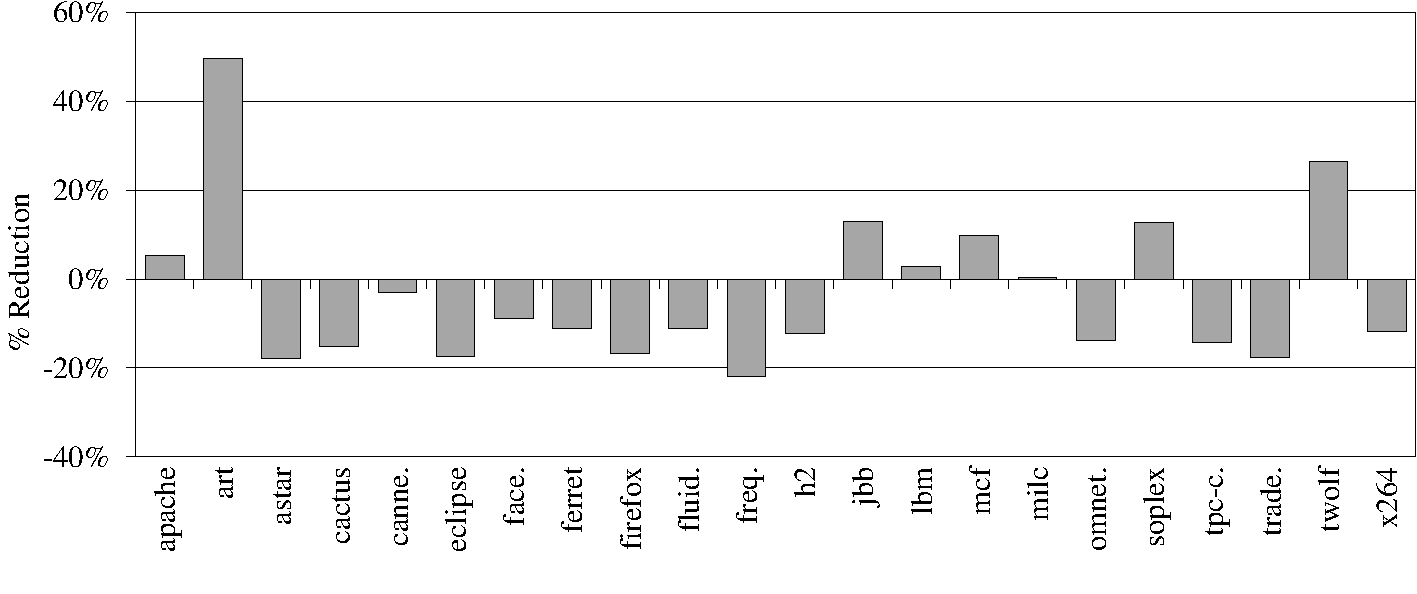
\includegraphics[width=\textwidth]{files/Plots/08-ExtraStage.pdf}
  \caption[Extra Cache Pipeline Stage Performance]{Percentage reduction in cycle time for all applications with with addition of an extra cache pipeline stage to accommodate for the \AC\ look-up overhead. positive bars indicate better performance. Negative bars indicate degradation in performance.}
  \label{fig:extra_cache_pipeline_stage}
\end{figure}

\subsection{Off-chip L2$\leftrightarrow$Memory energy}
The L2's higher cache capacity makes it less susceptible to pollution and provides less opportunity for improving miss rate. In such cases, the \AC\ keeps out unused words and reduces off-chip bandwidth and thereby off-chip energy. We assume that the off-chip DRAM can provide adaptive granularity transfers for \AC{}'s L2 refills as in~\cite{Yoon_Jeong_Erez_2011}. The DRAM model used was presented in a recent study~\cite{exascale} and consumes 0.5nJ per word transferred off-chip. The low spatial locality applications see a dramatic reduction in off-chip energy. For example, twolf sees a 93\% reduction. On commercial workloads the off-chip energy decreases by 31\% and 24\% respectively. Even for applications with high cache utilization, off-chip energy decreases by 15\%.

\begin{figure}[h]
  \centering
  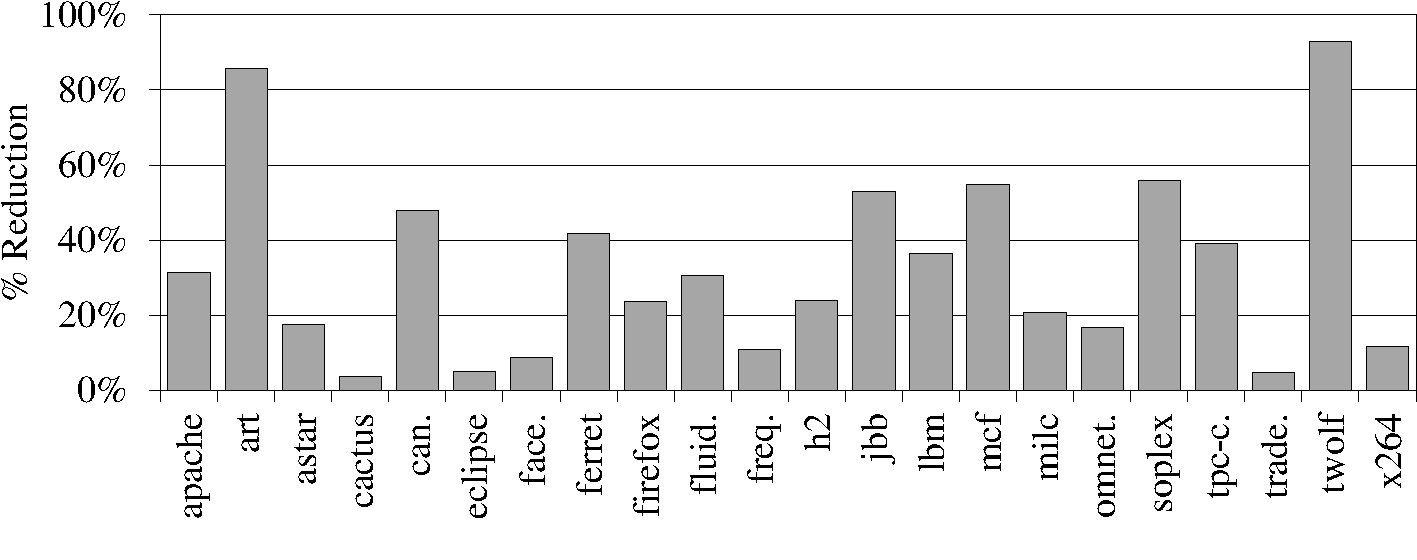
\includegraphics[width=\textwidth]{files/Plots/08-Oracle-OffChip-Energy.pdf}
  \caption[Off-Chip Energy Reduction]{Off chip energy reduction for all applications. Higher bars indicate greater savings in energy.}
  \label{fig:offchip_energy}
\end{figure}


\section{Spatial Predictor Trade-offs}
\label{sec:spatial_predictor_tradeoffs}

The effectiveness of spatial pattern prediction is evaluated in this section. In the table-based approach, a pattern history table records spatial patterns from evicted blocks and is accessed using a prediction index. The table-driven approach requires careful consideration of the following: prediction index, predictor table size and training period. The effects are quantified by comparing the predictor against a baseline fixed-granularity cache. A baseline 64K cache is used since it induces enough misses and evictions to highlight the predictor trade-offs clearly.

\subsection{Predictor Indexing} 

A critical choice with the history-based prediction is the selection of the predictor index. Two types of predictor indexing were explored:
\begin{itemize}[noitemsep]
  \item a program counter based(\code{PC}) approach\cite{chen-hpca-2004} based on the intuition that fields in a data structure are accessed by specific PCs and tend to exhibit similar spatial behavior. The tag includes the PC and the critical word index: $((PC>>3)<<3)+\frac{(addr\%64)}{8}$.
  \item a \textit{Region}-based (\code{REGION}) approach that is based on the intuition that similar data objects tend to be allocated in contiguous  regions of the address space and tend to exhibit similar spatial behavior. 
\end{itemize}

The miss rate and bandwidth properties of both the \code{PC} (256 entries, fully associative) and \code{REGION} (1024 entries, 4KB region size) predictors were compared. The size of the table used in each predictor was selected as the optimal found by empirical analysis for each predictor type.  For all applications apart from cactus (a high spatial locality application), \code{REGION}-based prediction tends to overfetch and waste bandwidth as compared to \code{PC}-based prediction, which has 27\% less bandwidth consumption on average across all applications. For 17 out of 22 applications, \code{REGION}-based prediction shows 17\%  better MPKI on average (max: 49\% for cactus). For 5 applications (apache, art, mcf, lbm, and omnetpp), \code{PC} has better accuracy when predicting the spatial behavior of cache blocks than \code{REGION} and demonstrates a 24\% improvement in MPKI (max: 68\% for omnetpp).

\subsection{Predictor Table}

The organization and size of the pattern table was studied using the \code{REGION} predictor. The following parameters were evaluated :
\begin{itemize}[noitemsep]
  \item region size, which directly correlates with the coverage of a fixed-size table
  \item the size of the predictor table
  \item the number of bits required to represent the spatial pattern.
\end{itemize}

Large region sizes effectively reduce the number of regions in the working set and require a smaller predictor table. However, a larger region is likely to have more blocks that exhibit varied spatial behavior and may pollute the pattern entry.  Increasing the region size from 1KB (4096 entries) to 4KB (1024 entries), the 4KB region granularity decreased miss rate by 0.3\% and increased bandwidth by 0.4\% even though both tables provide the same working set coverage (4MB).  Fixing the region size at 4KB, the benefits of an unbounded table were studied.  Compared to a 1024 entry table (\code{FINITE} in Figure~\ref{fig:Predictor_All_Apps}), the unbounded table increases miss rate by 1\% and decreases bandwidth by 0.3\% . A 1024 entry predictor table (4KB region granularity per-entry) suffices for most applications. Organizing the 1024 entries as a 128-set$\times$8-way table suffices to eliminate associativity related conflicts ($<$0.8\% evictions due to lack of ways).

\begin{figure}[h]
  \centering
    \subfloat[Misses Per Kilo Instructions]{
      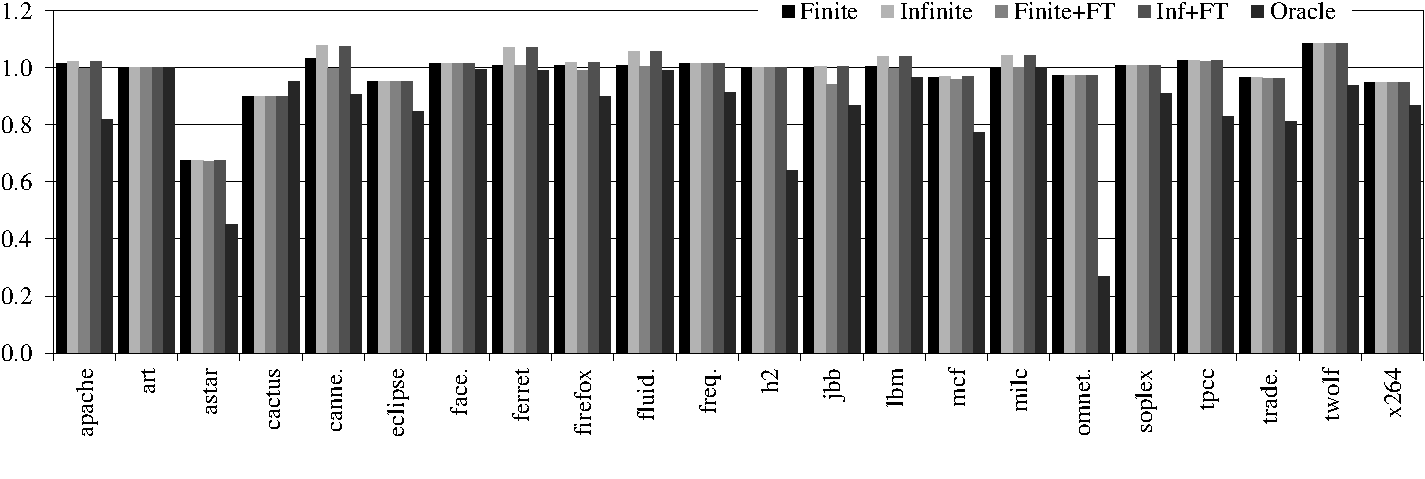
\includegraphics[width=\textwidth]{files/Plots/08-Predictor-MPKI.pdf}
    }
    
    \subfloat[Bandwidth]{
      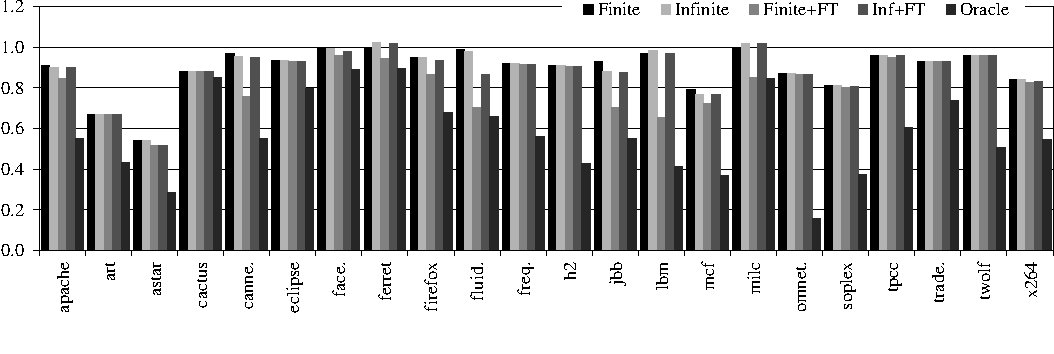
\includegraphics[width=\textwidth]{files/Plots/08-Predictor-BW.pdf}
    }
    \caption[Predictor Performance]{ The charts above show the performance of the different types of \AC\ predictors in terms of misses per kilo instructions and miss bandwidth for a 64K L1 equivalent scaled to the performance of a fixed granularity conventional cache. \\ \\
      \code{FINITE}: \code{REGION} predictor (1024 entry table and 4K region size). \\
      \code{INFINITE}: Unbounded predictor table (\code{REGION} predictor). \\ 
      \code{FINITE+FT}: \code{FINITE} with hints for prediction on compulsory misses (first touches). \\
      \code{INF+FT}: \code{INFINITE} with hints for prediction on compulsory misses (first touches). \\
      \code{HISTORY}: Uses spatial pattern hints collected at eviction from a prior run. 
    }
    \label{fig:Predictor_All_Apps}
\end{figure}

\clearpage

Focusing on the number of bits required to represent the pattern table, the use of 4-bit saturation counters (instead of 1-bit bitmaps) was evaluated. The saturation counters seek to avoid pattern pollution when blocks with varied spatial behavior reside in the same region. Interestingly, it was found that it is more beneficial to use 1-bit bitmaps for the majority of the applications (12 out of 22) as the hysteresis introduced by the counters increases training period.  

To summarize, it was found that a \code{REGION} predictor with region size 4KB and 1024 entries can predict the spatial pattern in a majority of the applications. CACTI indicates that the predictor table can be indexed in 0.025ns and requires 2.3pJ per miss indexing.

\subsection{Spatial Pattern Training} 

A widely-used approach to training the predictor is to harvest the word usage information on an eviction. Unfortunately, evictions may not be frequent, which means the predictor's training period tends to be long, during which the cache performs less efficiently and/or that the application's phase has changed in the meantime. Particularly at the time of first touch (compulsory miss to a location), a global spatial access pattern is required due to lack of a specific pattern. The finite region predictor (\code{FINITE} in Figure~\ref{fig:Predictor_All_Apps}) that only predicts using eviction history is compared against a \code{FINITE+FT}: this adds the optimization of inferring the default pattern (from a prior run) when there is no predictor information. \code{FINITE+FT} demonstrates an avg. 1\% (max: 6\% for jbb) reduction in miss rate compared to \code{FINITE} and comes within 16\% the miss rate of \code{HISTORY}. In terms of bandwidth \code{FINITE+FT} can save 8\% of the bandwidth (up to 32\% for lbm) compared to \code{FINITE}. The percentage of first-touch accesses is shown in Table~\ref{table:Abs_Eval_Oracle}.  




\subsection{Predictor Summary}
\begin{itemize}
  \item For the majority of the applications (17/22) the address-region predictor with region size 4KB works well. However, five applications (apache, lbm, mcf, art, omnetpp) show better performance with PC-based indexing. For best efficiency, the predictor should adapt indexing to each application. 
  \item Updating the predictor only on evictions leads to long training periods, which causes loss in caching efficiency. Mechanisms to infer the default pattern based on global behavior demonstrated by resident cache lines need to be developed to solve this problem.
  \item The online predictor reduces MPKI by 7\% and bandwidth by 26\% on average relative to the conventional approach. However, it still has a 14\% higher MPKI and 38\% higher bandwidth relative to the \code{HISTORY}-based predictor, indicating room for improvement in prediction. 
  \item The 1024-entry (4K region size) predictor table imposes $\simeq$0.12\% energy overhead on the overall cache hierarchy energy since it is referenced only on misses.
\end{itemize}

\section{\AC\ Adaptivity}
\label{sec:adaptivity}

The \AC{} can adapt better than a conventional cache to the variations in spatial locality.

\subsection{Tuning RMAX for High Spatial Locality} 
\label{sec:tuning_rmax_for_high_spatial_locality}

A challenge often faced by conventional caches is the desire to widen the cache block (to achieve spatial prefetching) without wasting space and bandwidth in low spatial locality applications. 3 specific applications are studied: milc and tradesoap have good spatial locality while soplex has poor spatial locality. With a conventional 1M cache, when the block size is widened from 64 to 128 bytes, milc and tradesoap experience a 37\% and 39\% reduction in miss rate. However, soplex's miss rate increases by 2$\times$ and bandwidth by 3.1$\times$.

The \AC{} can support \AB{}s with granularity 1---RMAX words (RMAX: maximum block size). When we increase RMAX from 64 bytes to 128 bytes, miss rate reduces by 37\% for milc and 24\% for tradesoap, while simultaneously lowering bandwidth by 7\%. Unlike the conventional cache, the \AC\ is able to adapt to poor spatial locality: soplex experiences only a 2\% increase in bandwidth and 40\% increase in miss rate.

\begin{figure}[!ht]
  \centering
  \vspace{10pt}
  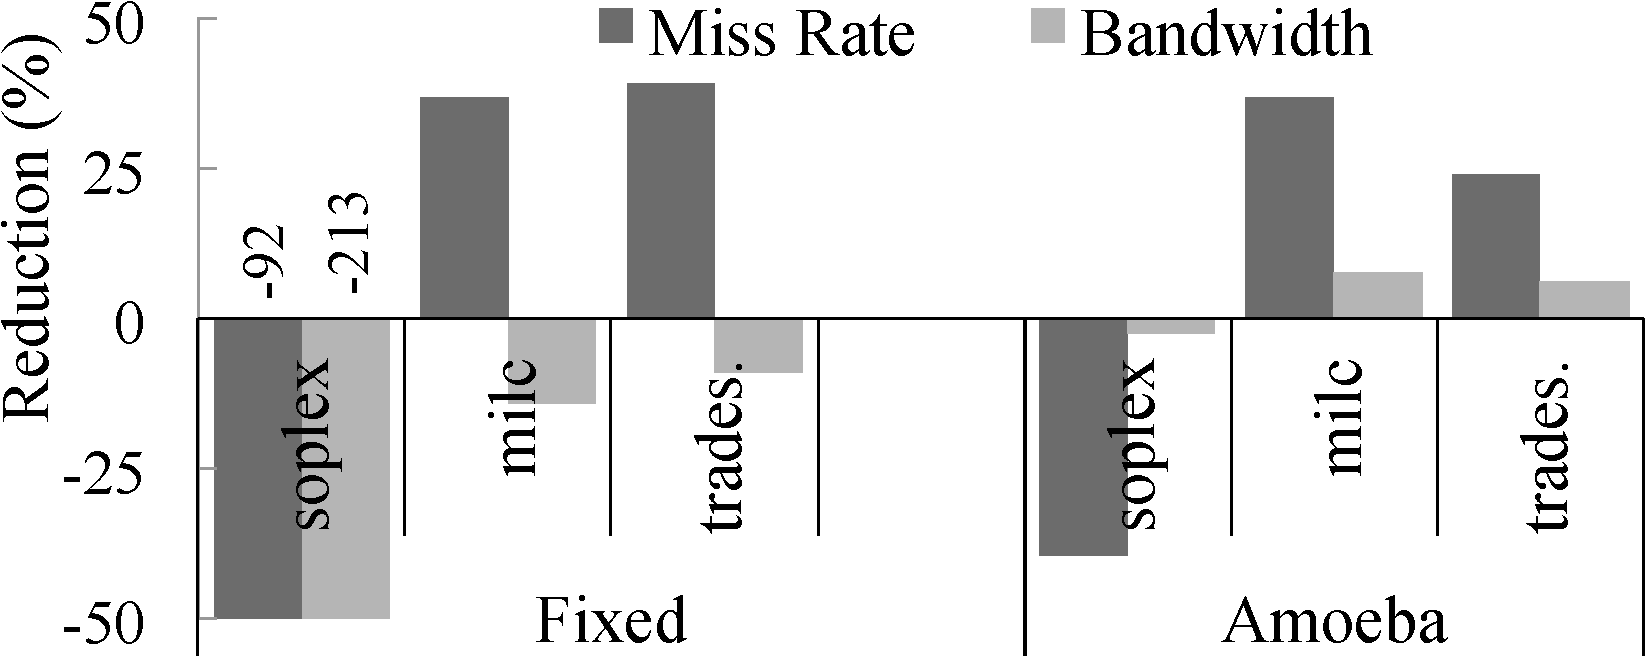
\includegraphics[width=0.7\textwidth]{files/Plots/08-Bar-Fixed-RMAX.pdf}
  \label{fig:rmax}
  \caption[\AC\ Adaptivity]{Effect of increase in block size from 64 to 128 bytes in a 1 MB cache}
 
\end{figure}

\subsection{Predicting Strided Accesses} 

Many applications (e.g.,firefox and canneal) exhibit strided access patterns, which touch a few words in a block before accessing another block. Strided accesses patterns introduce intra-block holes (untouched words). For instance, canneal accesses $\simeq$10K distinct fixed granularity cache blocks  with a specific access pattern, \textbf{[{-}{-}x{-}{-}x{-}{-}]} (\textbf{x} indicates $i^{th}$ word has been touched). 

%!TEX root=/home/ska124/Dropbox/Thesis/thes-full.tex
\begin{table}[!htb]
  \centering
  \begin{tabular}{|l|c|c|c|c| }
    \hline
    & \multicolumn{2}{c|}{canneal} &  \multicolumn{2}{c|}{firefox} \\
    \hline
    & Miss Rate & BW & Miss Rate & BW\\
    \hline
    Policy-Miss & 10.31\% & 81.2\% & 11.18\% & 47.1\%\\
    \hline
    Policy-BW & --20.08\% & 88.09\% & --13.44\% & 56.82\%\\
    \hline
    Spatial Patterns & \multicolumn{2}{c|}{\textbf{[{-}{-}x{-}{-}x{-}{-}]
        [x{-}{-}x{-}{-}{-}{-}]}} &
    \multicolumn{2}{c|}{\textbf{[{-}x{-}{-}x{-}{-}{-}]
        [x{-}{-}{-}x{-}{-}{-}]}} \\
    \hline
    \multicolumn{4}{c}{--: indicates Miss or BW higher than Fixed.}
  \end{tabular}
  \caption{Predictor Policy Comparison}
  \label{table:predictor_policy}
\end{table}

Any predictor that uses the access pattern history has two choices when an access misses on word 3 or 6 a) A miss oriented policy (Policy-Miss) may refill the entire range of words 3--6 and eliminate the secondary miss but bring in untouched words 4--5, increasing bandwidth, and b) a bandwidth focused choice (Policy- BW) that refills only the requested word but will incur more misses. Table~\ref{table:predictor_policy} compares the two contrasting policies for \AC{} (relative to a Fixed granularity baseline cache). Policy-BW saves 9\% bandwidth compared to Policy-Miss but suffer 25-30\% higher miss rate.

\section{\AC\ vs other approaches}
\label{sec:otherapproaches}

The \AC\ is compared against four approaches:

\begin{itemize}
  \item \textbf{Fixed-2x}: The baseline is a fixed granularity cache 2$\times$ the capacity of the other designs (64B block).
  \item \textbf{Sector}: The conventional sector cache design (as in IBM Power7~\cite{power7}): 64B block and a small sector size (16 bytes or 2 words).  This design targets optimal bandwidth. On any access, the cache fetches only the requisite sector, even though it allocates space for the entire line.
  \item \textbf{Sector-Pre}: Adds prefetching to \textbf{Sector}. This optimized design prefetches multiple sectors based on a spatial granularity predictor to improve the miss rate~\cite{kumar-isca-1998, pujara-hpca-2006}.
  \item \textbf{Multi\$}: Combines features from line distillation~\cite{Qureshi:2007:LDIS} and spatial-temporal    caches~\cite{Gonzalez:1995:DCM:224538.224622}. It is an aggressive design that partitions a cache into two: a line organized cache (LOC) and a word-organized cache (WOC). At insertion time, Multi\$ uses the spatial granularity hints to direct the cache to either refill words (into the WOC) or the entire line. Two design points are investigated: 50\% of the cache as a WOC (Multi\$-50) and 25\% of cache as a WOC (Multi\$-25).
\end{itemize}

Sector, Sector-Pre, Multi\$, and \AC\ all use the same spatial predictor hints. On a demand miss, they prefetch all the sub-blocks needed together. Prefetching only changes the timing of an access; it does not change the miss bandwidth and cannot remove the misses caused by cache pollution.

\subsection{Energy and Storage}
The sector approaches impose low hardware complexity and energy penalty. To filter out unused words, the sector granularity has to be close to word granularity; 2 words per sector leads to a storage penalty of $\simeq$64KB for a 1MB cache. In Multi\$, the WOC increases associativity to the number of words/block.  Multi\$-25 partitions a 64K 4-way cache into a 48K 3-way LOC and a 16K 8-way WOC, increasing associativity to 11. For a 1M cache, Multi\$-50 increases associativity to 36.  Compared to Fixed, Multi\$-50 imposes over 3$\times$ increase in look-up latency, 5$\times$ increase in look-up energy, and $\simeq$4$\times$ increase in tag storage. \AC\ provides a more scalable approach to using adaptive cache lines since it varies the storage dedicated to the tags based on the spatial locality in the application.

\begin{figure}[!ht]
  \subfloat[64K - Low]{
    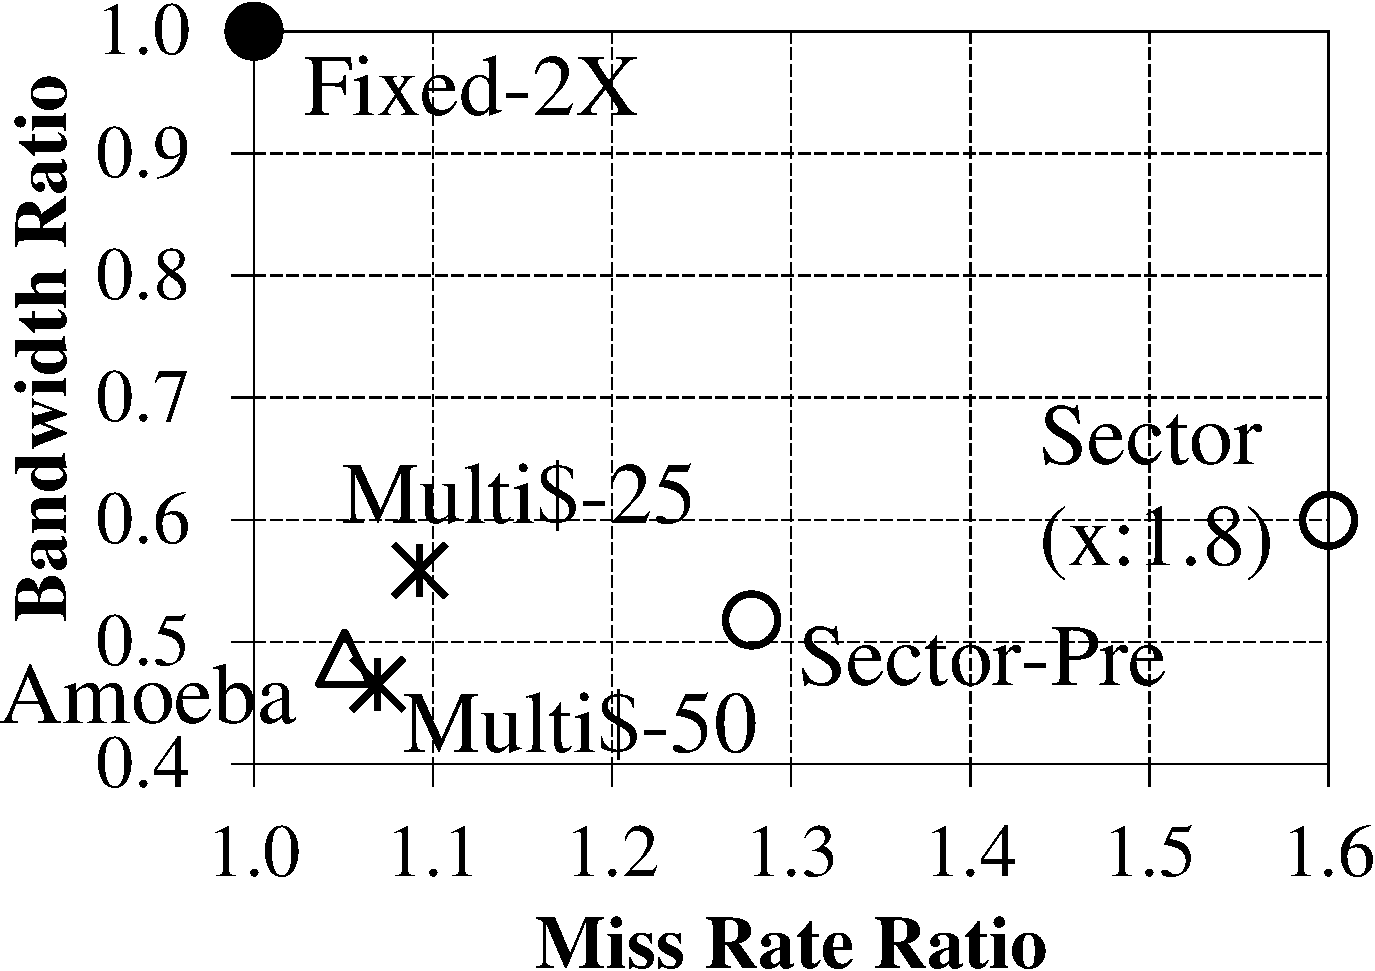
\includegraphics[width=0.5\textwidth]{files/Plots/08-Comparison-Scatter-64K-Low.pdf}
  }
  \subfloat[64K - Moderate]{
     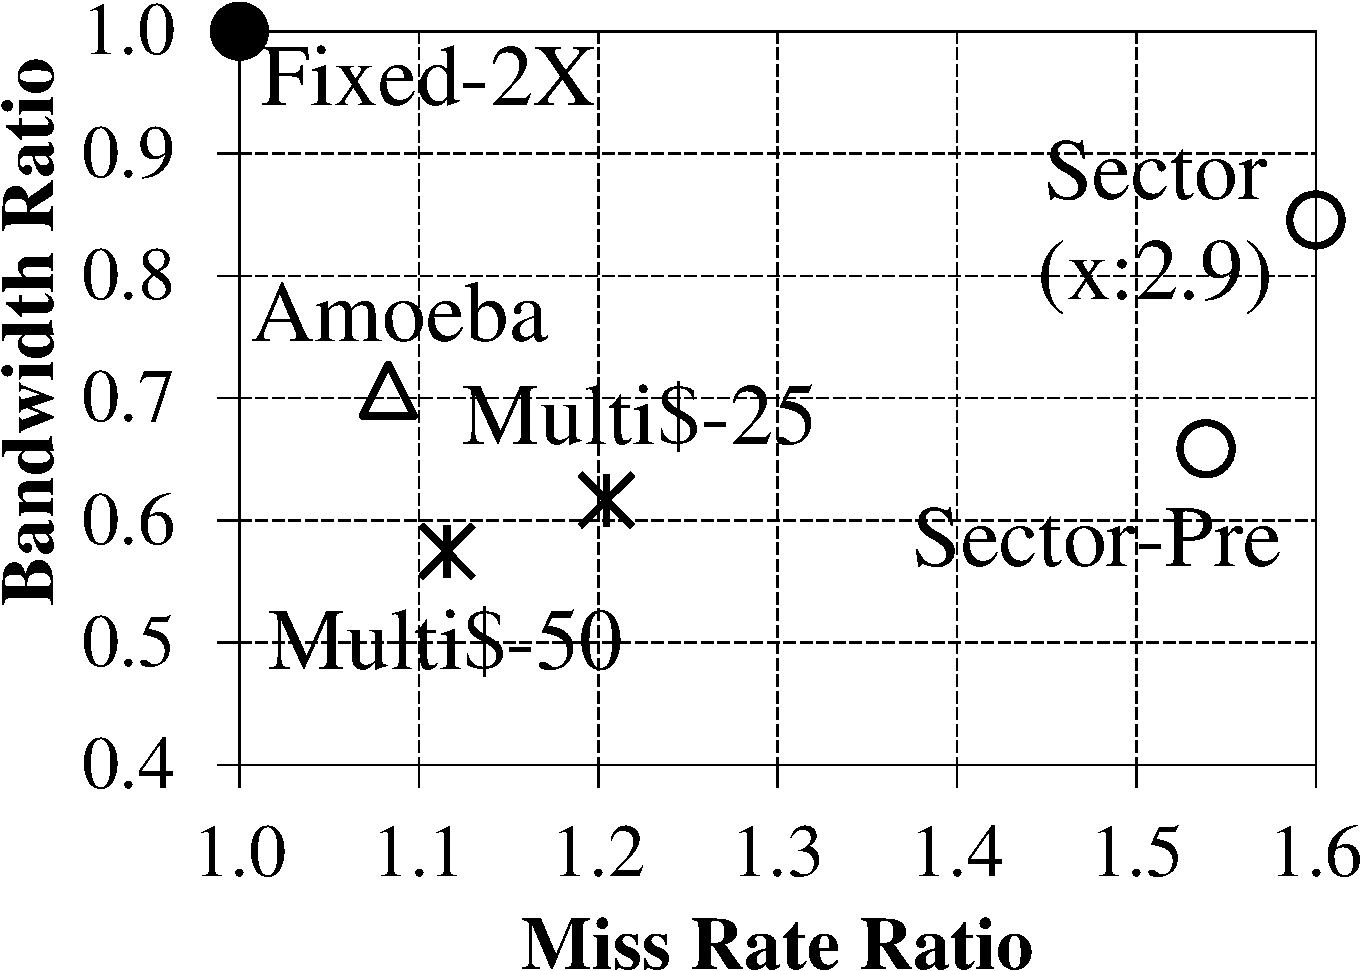
\includegraphics[width=0.5\textwidth]{files/Plots/08-Comparison-Scatter-64K-Moderate.pdf}
  }

  \subfloat[1M - Low]{
    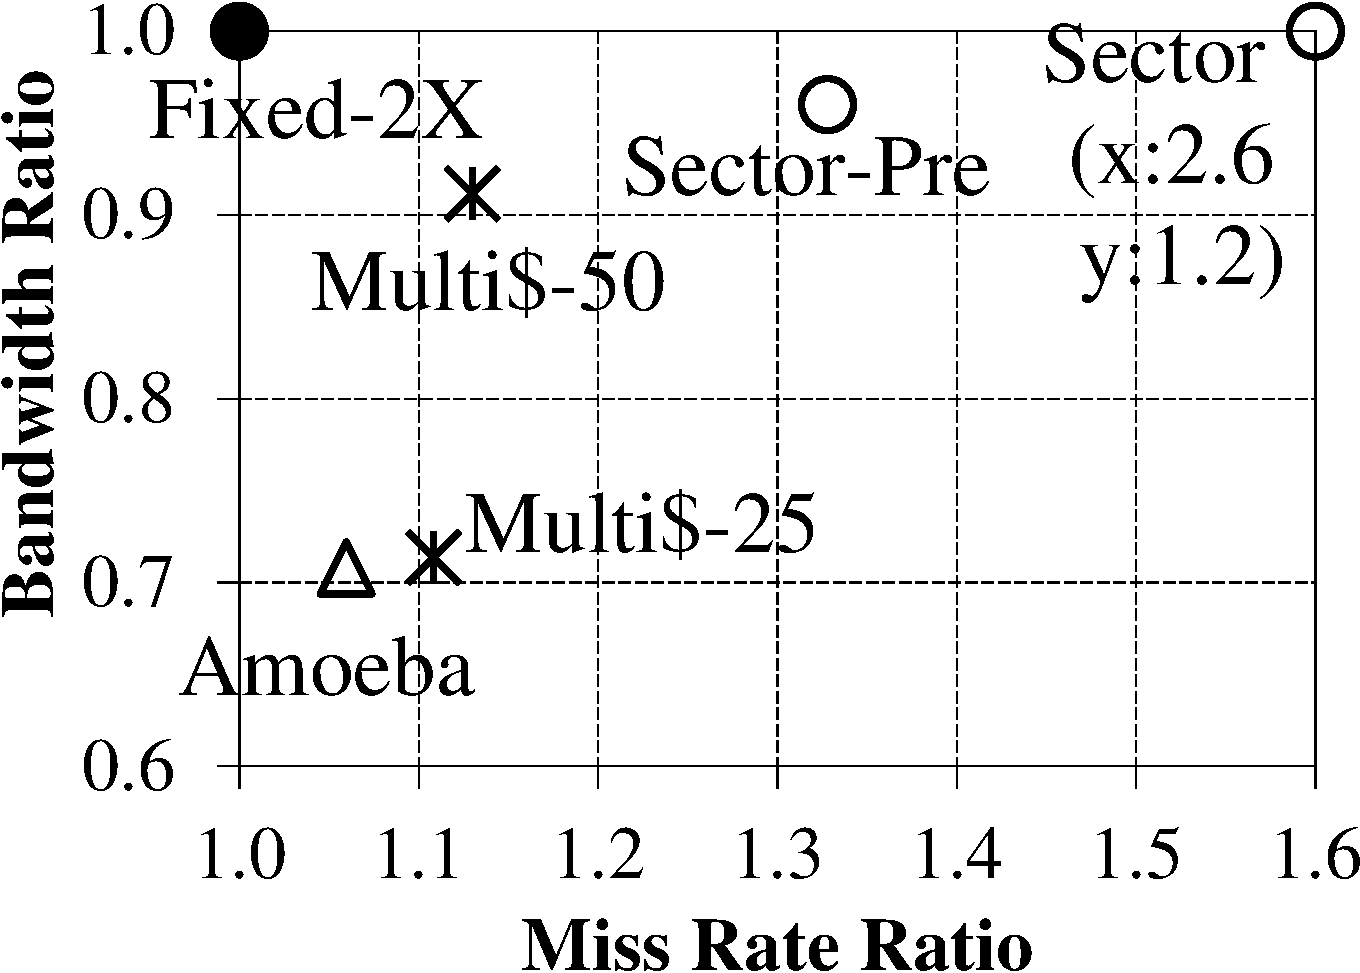
\includegraphics[width=0.5\textwidth]{files/Plots/08-Comparison-Scatter-1M-Low.pdf}
  }
  \subfloat[1M - Moderate]{
     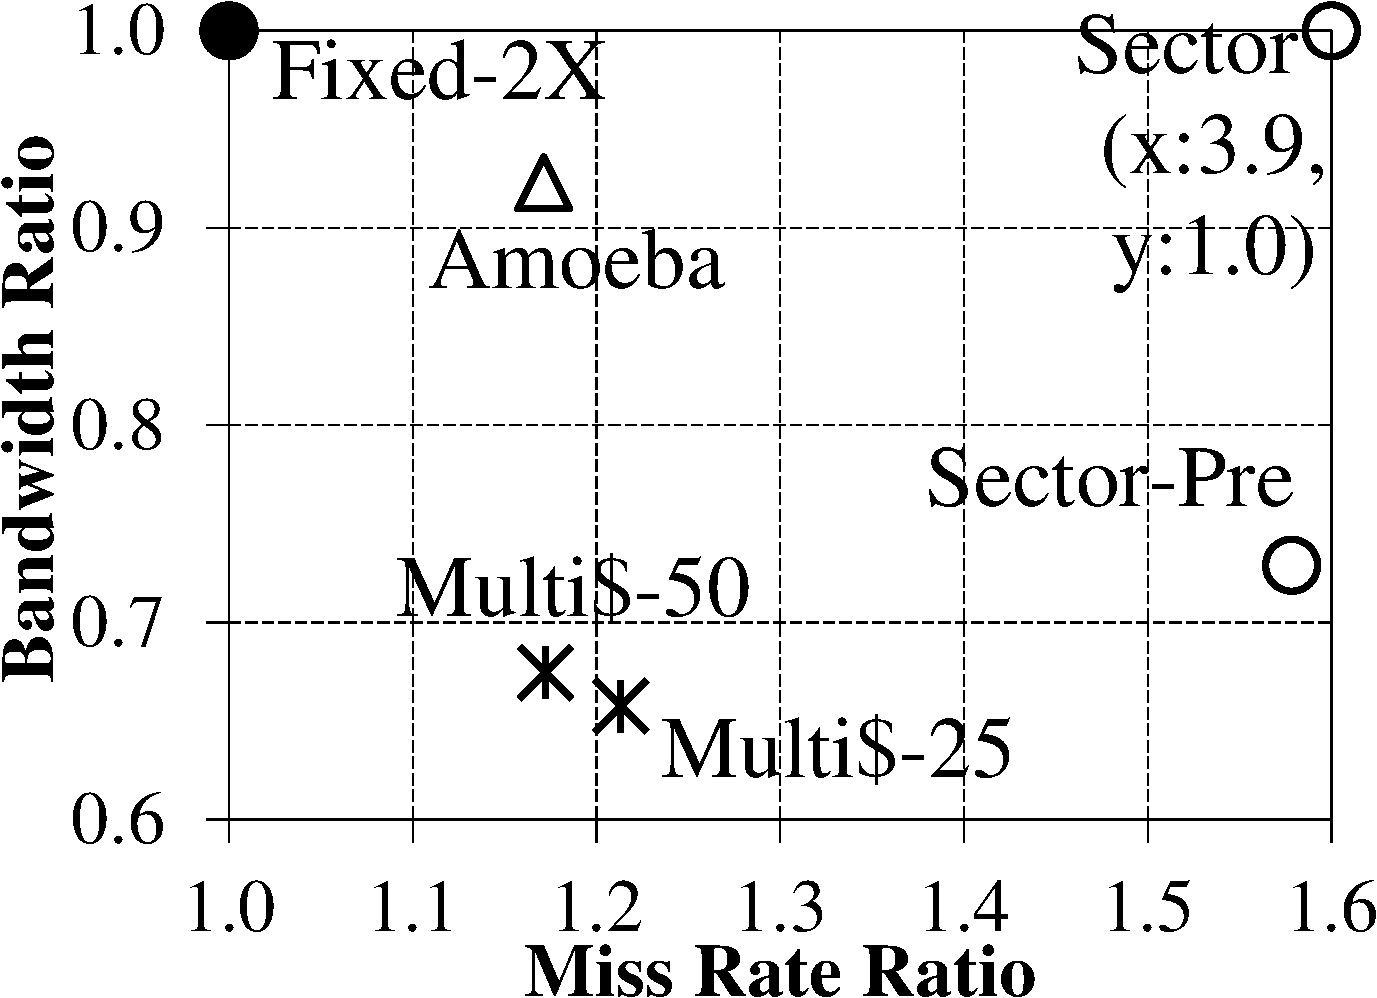
\includegraphics[width=0.5\textwidth]{files/Plots/08-Comparison-Scatter-1M-Moderate.pdf}
  }
  \caption[\AC\ Comparison]{Relative miss rate and bandwidth for different caches. Baseline (1,1) is the Fixed-2$\times$ design. \\
    Labels: {\bf \large $\bullet$} Fixed-2x, {\large \bf $\circ$}
    Sector approaches. {\large \bf $\ast$} : Multi\$, $\bigtriangleup$ Amoeba. \\ 
    (a),(b) 64K cache (c),(d) 1M cache. Note the different Y-axis scale for each group.}
  \label{fig:scatter_comp}
\end{figure}

\clearpage

\subsection{Miss Rate and Bandwidth}
Figure~\ref{fig:scatter_comp} summarizes the comparison for the moderate and low utilization groups of applications. For the high utilization group, all designs other than Sector have comparable miss rates. \AC\ improves miss rate to within 5\%---6\% of the Fixed-2$\times$ for the low group and within 8\%---17\% for the moderate group. Compared to the Fixed-2$\times$, \AC\ also lowers bandwidth by 40\% (64K cache) and 20\% (1M cache). Compared to Sector-Pre (with prefetching), the \AC\ is able to adapt better with flexible granularity and achieves lower miss rate (up to 30\% for a 64K L1 and 35\% for a 1M LLC equivalent). Multi\$'s benefits are proportional to the fraction of the cache organized as a WOC; Multi\$-50 (18-way for 64K L1 and 36-way for 1M LLC) is needed to match the miss rate of \AC{}. Finally, in the moderate group, many applications exhibit strided access. Compared to Multi-\$'s WOC, which fetches individual words, the \AC\ increases bandwidth since it chooses to fetch the contiguous chunk in order to lower miss rate.

\clearpage

\section{Multicore Shared Cache}
\label{sec:multicore}

A shared \AC\ is evaluated. By dynamically varying the cache block size and keeping out unused words, the \AC\ effectively minimizes the footprint of an application. Minimizing the footprint helps multiple applications effectively share the cache space. Results are presented for experiments using a 1M shared \AC\ in a 4 core system. Table~\ref{table:multiprogrammed} shows the application mixes; application mixes are chosen across all groups. The change in miss rate is tabulated as miss rate per thread and the overall change in bandwidth for \AC\ with respect to a fixed granularity cache running the same mix. Minimizing the overall footprint enables a reduction in the miss rate of each application in the mix. The commercial workloads (SpecJBB and TPC-C) are able to make use of the space available and achieve a significant reduction in miss rate (avg: 18\%). Only two applications suffered a small increase in miss rate (x264 Mix 2: 2\% and ferret Mix 3: 4\%) due to contention. The overall L2 miss bandwidth significantly improves, showing 16\%---39\% reduction across all workload mixes. An \AC\ based shared cache design can effectively enable the shared cache to support more cores and increase overall throughput. The design space exploration of a coherent \AC\ is part of planned future work.

\begin{table}[!h]
  \vspace{10pt}
  \centering
  \begin{tabular}{|c|c|c|c|c|c|} 
      \hline
      & Miss  & Miss  & Miss  & Miss & BW \\
      \hline
      Mix & T1 & T2 & T3 & T4 & (All)\\
      \hline
      jbb$\times$2, tpc-c$\times$2 & 12.38\% & 12.38\% & 22.29\% &22.37\% & 39.07\% \\
      \hline
      firefox$\times$2, x264$\times$2 & 3.82\% & 3.61\% & --2.44\% & 0.43\% & 15.71\%\\
      \hline
      cactus, fluid., omnet., sopl. & 1.01\% & 1.86\% & 22.38\% & 0.59\% & 18.62\% \\
      \hline
      canneal, astar, ferret, milc & 4.85\% & 2.75\% & 19.39\% & --4.07\% & 17.77\%\\
      \hline
  \end{tabular}
  \caption[Multiprogrammed workloads on \AC{}]{\textbf{Multiprogrammed Workloads on 1M Shared \AC{}}: Percentage reduction in miss rate and bandwidth. \\ \\  
  --: indicates Miss or BW higher than Fixed. T1---T4, threads in the mix; in the order of applications in the mix. Baseline: Fixed granularity 1M conventional cache.}
  \label{table:multiprogrammed} 
\end{table}


%!TEX root=/home/ska124/Dropbox/Thesis/thes-full.tex
\begin{table}[h]
\centering
	\begin{tabular}{|c|c|c|c|c|c|c|c|c|}
	\hline
	 & \multicolumn{2}{c|}{MPKI} &  \multicolumn{2}{c|}{BW Bytes/1K} & CPI & \multicolumn{2}{c|}{Predictor Stats}  \\
	\hline
	          & L1        & L2    & L1$\longleftrightarrow$L2 & L2$\longleftrightarrow$Mem & & FT &  \\
	          & MPKI & MPKI & Bytes/1K & Bytes/1K & Cycles/Ins. & Miss \% &  Ins/Evict\\
	\hline
	apache    &    64.9 & 19.6    &    5,000  &    2,067         &  8.3  & 0.4 &   17 \\
	art       &    133.7  &    53.0    &    5,475  &    1,425    &  16.0 & 0.0 &   9 \\
	astar     &    0.9    &    0.3     &    70     &    35       &  1.9  & 18.0 &  1,600 \\
	cactus    &    6.9    &    4.4     &    604    &    456      &  3.5  & 7.5 &   162 \\
	canne.    &    8.3    &    5.0     &    486    &    357      &  3.2  & 5.8 &   128 \\
	eclip.    &    3.6    &    $<$0.1  &    433    &    $<$1     &  1.8  & 0.1 &   198 \\
	faces.    &    5.5    &    4.7     &    683    &    632      &  3.0  & 41.2 &  190 \\
	ferre.    &    6.8    &    1.4     &    827    &    83       &  2.1  & 1.3 &   156 \\
	firef.    &    1.5    &    1.0     &    123    &    95       &  2.1  & 11.1 &  727 \\
	fluid.    &    1.7    &    1.4     &    138    &    127      &  1.9  & 39.2 &  629 \\
	freqm.    &    1.1    &    0.6     &    89     &    65       &  2.3  & 17.7 &  994 \\
	h2        &    4.6    &    0.4     &    328    &    46       &  1.8  & 1.7 &   154 \\
	jbb       &    24.6   &    9.6     &    1,542  &    830      &  5.0  & 10.2 &  42 \\
	lbm       &    63.1   &    42.2    &    3,755  &    3,438    &  13.6 & 6.7 &   18 \\
	mcf       &    55.8   &    40.7    &    2,519  &    2,073    &  13.2 & 0.0 &   19 \\
	milc      &    16.1   &    16.0    &    1,486  &    1,476    &  6.0  & 2.4 &   66 \\
	omnet.    &    2.5    &    $<$0.1  &    158    &    $<$1     &  1.9  & 0.0 &   458 \\
	sople.    &    30.7   &    4.0     &    1,045  &    292      &  3.1  & 0.9 &   35 \\
	tpcc      &    5.4    &    0.5     &    438    &    36       &  2.0  & 0.4 &   200 \\
	trade.    &    3.6    &    $<$0.1  &    410    &    6        &  1.8  & 0.6 &   194 \\
	twolf     &    23.3   &    0.6     &    1,326  &    45       &  2.2  & 0.0 &   49 \\
	x264      &    4.1    &    1.8     &    270    &    190      &  2.2  & 12.4 &  274 \\
	\hline                                  
	\end{tabular}                                                                       
                                                                       
\caption[Absolute performance statistics]{Abslute performance statistics for the \AC\ using a \code{Region} predictor(infinite table size) with predictions for compulsory misses serviced using data collected from a prior run of the application. Higher value for Ins/Evict indicates predictor training takes longer. \\ \\
	\textbf{MPKI} : Misses / 1K instructions. \\
	\textbf{BW}: Number of words / 1K instructions. \\
	\textbf{CPI}: Clock cycles per instruction. \\
	\textbf{FT}: Percentage of misses that are compulsory misses.  \\
	\textbf{Ins/Evict}: Number of instructions between evictions. 
}
\label{table:Abs_Eval_Oracle}                                        
\end{table}                                                          
\clearpage

% First Touch info for Inf Table
% 0.4
% 0.0
% 18.0
% 7.5
% 5.8
% 0.1
% 41.2
% 1.3
% 11.1
% 39.2
% 17.7
% 1.7
% 10.2
% 6.7
% 0.0
% 2.4
% 0.0
% 0.9
% 0.4
% 0.6
% 0.0
% 12.4

% First Touch info for 1K Table
% 16.0
% 0.0
% 20.1
% 9.5
% 44.0
% 0.1
% 76.3
% 20.1
% 44.9
% 86.6
% 19.3
% 2.7
% 55.4
% 57.0
% 13.6
% 93.2
% 0.0
% 1.9
% 5.1
% 0.6
% 0.0
% 19.0


% Instructions per Eviction data for Oracle 64K

% 17
% 9
% 1,600
% 162
% 128
% 198
% 190
% 156
% 727
% 629
% 994
% 154
% 42
% 18
% 19
% 66
% 458
% 35
% 200
% 194
% 49
% 274

%!TEX root=/home/ska124/Dropbox/Thesis/thes-full.tex

%%%%%%%%%%%%%%%%%%%%%%%%%%%%%%%%%%%%%%%%%%%%%%%%%
%
%     Chapter 6
%
%%%%%%%%%%%%%%%%%%%%%%%%%%%%%%%%%%%%%%%%%%%%%%%%

\chapter{Conclusion}
\label{chap:conclusions}

In this chapter the primary findings are summarized and describe future work motivated by these findings. 

\section{Conclusions}

This dissertation presents a novel architecture for an adaptive granularity cache memory system, the \AC{}. The \AC\ adapts to the requirements of the application to cache variable sized \AB{}s. This is achieved by eliminating the tag array and storing tags and variable granularity data within the same SRAM data array. The \AC\ keeps out the unused words, thus increasing caching efficiency. Experimental evaluations show a reduced miss rate, improvement in performance and reduced consumption in energy. 

Compared to a fixed granularity cache, improves cache utilization to 90\% - 99\% for most applications, saves miss rate by up to 73\% at the L1 level and up to 88\% at the LLC level, and reduces miss bandwidth by up to 84\% at the L1 and 92\% at the LLC. Correspondingly reduces on-chip memory hierarchy energy by as much as 36\% and improves performance by as much as 50\%.

We conclude that the \AC\ is a plausible design which can be implemented with considerations discussed in \S~\ref{sec:hardware_complexity}. We believe the \AC\ is a promising step towards more flexible hardware to suit the ever changing needs of software and becomes more important with added significance of energy efficient hardware.

\section{Future Work}
The possible avenues of exploration based on the current \AC\ infrastructure are described as follows.

\paragraph{Adaptive Granularity Cache Coherence}: Prior work which adapt existing schemes such as sector caches~\cite{Rothman_Smith_2000} to support sub-block coherence~\cite{Subblock_Coherence,minerva}, show the viability of extending \AC\ to a full multicore cache coherence protocol. As previously described in \S~\ref{sec:coherence}, the important issues to tackle when building a directory based \AC\ protocol are :
\begin{itemize}[noitemsep]
	\item Maintaining precise information in the coherence directory
	\item Supporting variable granularity read sharing
	\item Determining the optimal write invalidation granularity
\end{itemize}
Based on the enumerated points, exploring the design space for an \AC\ based cache coherence protocol is part of planned future work. 

\paragraph{Replacement Policies}: Investigating more intelligent replacement policies for the \AC\ can also make for interesting future work. Currently the Pseudo-LRU policy described in \S~\ref{sec:replacement_policy} has been adapted for use in the \AC\ and leaves room for improvement. Inspiration can be drawn from the \textit{Generational Replacement Policy} described by Hallnor et al.\cite{Hallnor_Reinhardt_2000} for a customized replacement policy for the \AC{}. Another issue which a replacement policy can address is the fragmentation within a cache set due to frequent changes in granularity required by the application. A replacement policy tailored for the \AC\ should be able to reduce the unnecessary evictions due to fragmentation within a cache set.

\paragraph{Cache Compression}: Cache compression is an area of work which can benefit from the flexibility of the \AC{} whilst storing variable granularity cache blocks. Prior work such as the compressed memory hierarchy by Hallnor et al.\cite{Hallnor04acompressed} can be suitably modified to use an \AC\ as the substrate.



%%%  appendices, if any
% \begin{appendices}
% %!TEX root=/home/ska124/Dropbox/Thesis/thes-full.tex
%% Copyright 1998 Pepe Kubon
%%
%% `appone.tex' --- 1st appendix for thes-full.tex, thes-short-tex from
%%                  the `csthesis' bundle
%%
%% You are allowed to distribute this file together with all files
%% mentioned in READ.ME.
%%
%% You are not allowed to modify its contents.
%%

%%%%%%%%%%%%%%%%%%%%%%%%%%%%%%%%%%%%%%%%%%%%%%%%%
%
%        Appendix 1
%
%%%%%%%%%%%%%%%%%%%%%%%%%%%%%%%%%%%%%%%%%%%%%%%%

% \chapter{}
\label{app:spacing}


% %!TEX root=/home/ska124/Dropbox/Thesis/thes-full.tex
%% Copyright 1998 Pepe Kubon
%%
%% `apptwo.tex' --- 2nd appendix for thes-full.tex from
%%                  the `csthesis' bundle
%%
%% You are allowed to distribute this file together with all files
%% mentioned in READ.ME.
%%
%% You are not allowed to modify its contents.
%%

%%%%%%%%%%%%%%%%%%%%%%%%%%%%%%%%%%%%%%%%%%%%%%%%%
%
%        Appendix 2
%
%%%%%%%%%%%%%%%%%%%%%%%%%%%%%%%%%%%%%%%%%%%%%%%%

\chapter{Illustrating Lists}\label{app:lists}
\index{formatting of Lists}

This appendix is present only in the full version of the thesis. It
illustrates in more detail the formatting of the Lists of Tables,%
\index{List of Tables}\index{List of Figures} Figures, etc. In
addition, it also illustrates the use of the ``other list'' facility
of \textsf{csthesis.sty}\index{csthesis.sty@\textsf{csthesis.sty}}.
Let us start with the latter.

\section{List of Programs}
\index{List of Programs}

In the preamble of \texttt{thes-full.tex}%
\index{thes-full.tex@\texttt{thes-full.tex}}, a new type of a floating
environment---\texttt{program}%
\index{program environment@\texttt{program} environment}---is defined,
together with the \verb+\otherlist+%
\index{otherlist@\texttt{\symbol{'134}otherlist}} command for
typesetting the List of Programs. The list is formatted in the same
way as the lists of Figures and Tables, and an appropriate entry is
added into Contents.

Because programs are defined here as floating environments, they are
typeset with the same (tighter) line-spacing%
\index{spacing in programs} as figures and tables:

\begin{program}[htbp]
  \begin{center}
    This shows that single line spacing\\
    is used inside programs.
    \caption{Example of the new \texttt{program} environment\label{prog1}}
  \end{center}
\end{program}
%
\vspace*{-.3in}
\begin{program}[htbp]
  \begin{center}
    A second example of a program environment.
    \caption{Second program\label{prog2}}
  \end{center}
\end{program}

\section{Formatting of Lists}

The tables (figures, programs, etc.) are organized and sorted by
chapters (appendices), with additional small vertical space separating
the chapter blocks. To illustrate this, I include two new tables here
(see List of Tables, etc., in the beginning of the thesis for the
result)\index{formatting of Lists}:

\begin{table}[htbp]
  \begin{center}
    To be silly or not to be silly\\
    \emph{that} is the question!
    \caption{First meaningless table in Appendix~\ref{app:lists}}
  \end{center}
\end{table}
%
\vspace*{-.3in}
\begin{table}[htbp]
  \begin{center}
    $F = nd^{2}$
    \caption{Second meaningless table in Appendix~\ref{app:lists}}
  \end{center}
\end{table}


% \end{appendices}

%%%%%%  bibliography
%!TEX root=/home/ska124/Dropbox/Thesis/thes-full.tex
%% Copyright 1998 Pepe Kubon
%%
%% `bibl.tex' --- bibliography for thes-full.tex, thes-short-tex from
%%                the `csthesis' bundle
%%
%% You are allowed to distribute this file together with all files
%% mentioned in READ.ME.
%%
%% You are not allowed to modify its contents.
%%

%%%%%%%%%%%%%%%%%%%%%%%%%%%%%%%%%%%%%%%%%%%%%%%%
%
%       Bibliography
%
%%%%%%%%%%%%%%%%%%%%%%%%%%%%%%%%%%%%%%%%%%%%%%%%

\nocite{*}     % everything cited automatically

\renewcommand{\baselinestretch}{\tighttextstretch} %% get smaller spacing
\normalsize

\bibliographystyle{plain}   %% dash under repeated name, von ignored
\addcontentsline{toc}{chapter}{Bibliography}
\typeout{Bibliography}
\bibliography{files/thes-both}
\renewcommand{\baselinestretch}{\textstretch} %% get normal spacing
\normalsize



%%%%%%  index
% %!TEX root=/home/ska124/Dropbox/Thesis/thes-full.tex
%% Copyright 1998 Pepe Kubon
%%
%% `ind.tex' --- index for thes-full.tex from
%%               the `csthesis' bundle
%%
%% You are allowed to distribute this file together with all files
%% mentioned in READ.ME.
%%
%% You are not allowed to modify its contents.
%%

%%%%%%%%%%%%%%%%%%%%%%%%%%%%%%%%%%%%%%%%%%%%%%%%
%
%       Index
%
%%%%%%%%%%%%%%%%%%%%%%%%%%%%%%%%%%%%%%%%%%%%%%%%

\renewcommand{\baselinestretch}{\tighttextstretch} %% get smaller spacing
\normalsize

\addcontentsline{toc}{chapter}{Index}
\typeout{Index}
\printindex

\renewcommand{\baselinestretch}{\textstretch} %% get normal spacing
\normalsize



\end{document}

